\documentclass[12pt]{report} 
\usepackage{geometry}
 \geometry{
 a4paper,
 total={210mm,297mm},
 left=40mm,
 right=20mm,
 top=20mm,
 bottom=20mm,
 }
\usepackage{caption}
\usepackage{subcaption}

\usepackage{hyperref}

% Default fixed font does not support bold face
\DeclareFixedFont{\ttb}{T1}{txtt}{bx}{n}{10} % for bold
\DeclareFixedFont{\ttm}{T1}{txtt}{m}{n}{10}  % for normal

% Custom colors
\usepackage{color}
\definecolor{deepblue}{rgb}{0,0,0.5}
\definecolor{deepred}{rgb}{0.6,0,0}
\definecolor{deepgreen}{rgb}{0,0.5,0}

\usepackage{listings}

% Python style for highlighting
\newcommand\pythonstyle{\lstset{
language=Python,
basicstyle=\ttm,
otherkeywords={self, run, kill_agents,reproduce_agents,random.choice,random.random,copy.deepcopy, assign_strategies,randomly_pair_agents,strategies_to_utilities,interact},             % Add keywords here
keywordstyle=\ttb\color{deepblue},
emph={Genetic, Agents, BiMatrixRandomEnv,__init__,Simulation},          % Custom highlighting
emphstyle=\ttb\color{deepred},    % Custom highlighting style
stringstyle=\color{deepgreen},
breaklines=true,
numbers=left,
numberstyle=\footnotesize,
stepnumber=1,
numbersep=8pt,
showstringspaces=false            
}}

% Python for inline
\newcommand\pythoninline[1]{{\pythonstyle\lstinline!#1!}}

% Python for external files
\newcommand\pythonexternal[2][]{{
\pythonstyle
\lstinputlisting[#1]{#2}}}

%Tikz package
\usepackage{tikz}
\usetikzlibrary{shapes,arrows}
\usetikzlibrary{calc}

% Define block styles
\tikzstyle{envblock} = [rectangle, draw, fill=gray!20, 
    text width=13em, text centered, rounded corners, minimum height=4cm]
\tikzstyle{algblock} = [rectangle, draw, fill=purple!40, 
    text width=14em, text centered, rounded corners, minimum height=4em]
\tikzstyle{ageblock} = [rectangle, draw, fill=orange!20, 
    text width=14em, text centered, rounded corners, minimum height=4em]
\tikzstyle{simblock} = [rectangle, draw, fill=green!30, 
    text width=13.5em, text centered, rounded corners, minimum height=6em]
\tikzstyle{geneblock} = [rectangle, draw, fill=green!30, 
    text width=12em, text centered, rounded corners, minimum height=2em]
\tikzstyle{line} = [draw, -latex']

\usepackage{amsmath}
\usepackage{amssymb}

\usepackage{graphicx} 
\graphicspath{ {images/} }
\usepackage{float}

%\usepackage{fullpage}
\usepackage[parfill]{parskip}


\newpage
\begin{document}

\thispagestyle{empty}
\begin{titlepage}
	\begin{center}
	\vspace*{1cm}
	\thispagestyle{empty}

	\includegraphics[scale=1.5]{cardifflogo}

	\vspace{1.5cm}

	\Huge
	\textbf{Solving Normal form games by building a Python package that uses a genetic algorithm.}

	\vspace{1cm}

	\Large
	\textbf{Cesar Ivan Esparza Soto}
	
	\vspace{1.5cm}	

	\Large
	September 2015\\

	School of Mathematics\\

	Cardiff University\\

	\vfill	
	
	\normalsize
	A  dissertation submitted in partial fulfilment of the requirements for MSc (in Operational Research and Applied Statistics) by 			taught programme.
	\end{center}
\end{titlepage}

\pagenumbering{Roman}

\thispagestyle{empty}
\chapter*{Abstract}
The literature review can be found in the following section. Some history of Game theory will be mentioned, Nash equilibrium is briefly mentioned but still important since the concept of equilibrium is important to discuss in game theory, simple concept about normal form games, history of evolutionary game theory and an explanation of what evolutionary game theory is and the introduction of the concept of equilibrium in evolutionary game theory which is known as evolutionary stable strategies(ESS), and a brief explanation of the similarities with Nash equilibrium.

\thispagestyle{empty}
\chapter*{Dedication}
To my family
\thispagestyle{empty}
\chapter*{Declaration}
I declare that..
\thispagestyle{empty}
\chapter*{Acknowledgements}
I want to thank..

\newpage
\thispagestyle{empty}
\tableofcontents

\newpage
\thispagestyle{empty}
\listoftables

\newpage
\thispagestyle{empty}
\listoffigures
 
\newpage
\pagenumbering{arabic}

\chapter*{Summary}
In this project a review of  ``evolutionary game theory'' was presented, which is a subfield of game theory. Evolutionary game theory is the application of game theory to the concept of evolution. This was relevant for understanding, how seen from a biological sense, game theory can be applicable to concepts of survival of species. With this as a basic idea it is easier to understand the concept of the ``genetic algorithm'' used to create a python library for this project. The ``genetic algorithm'' used was simple, and it mainly uses concepts and assumptions from ``evolutionary game theory''. The algorithm basically consists in the creation of agents with characteristics. The approach taken for defining agents, was agent-based modelling, which main purpose is to simulate the how the interactions between different agents has an effect on the individual agent and in the whole system. The main characteristics for each agent are: each created agent has only one strategy which it will use until it is eliminated and by using this strategy the agent is capable of accumulating a utility. When the utility is high it will help it to endure during the simulation, and it will very likely be able to produce a copy of itself, consequently the strategy it passes on will be present in more agents during the simulation. On the other hand, agents with a low accumulated utility will probably disappear as the simulation progresses. Parameters that affected  the simulation were introduced, such as death rate, mutation rate, exploitation rate and initial distribution of strategies. For being able to build a simulation with all of the features mentioned ``Python'' was used which an object oriented programming language. Once a Python library capable of running simulations was created some of the most known games in game theory like prisoner's dilemma, matching pennies, battle of sexes and hawk-dove (in evolutionary game theory) were simulated. All these games were tested with different combination of parameters, to observe their individual behaviour. And peculiarities for each game, according to their types of equilibria (mixed or pure) were observed. After these games were tested an additional game was tested. This game was produced with a Python package called ``axelrod'', which allows simulate tournaments with predetermined strategies. From ``axelrod'' a payoff matrix was taken, this payoff matrix was transformed into a bimatrix and introduced into the Python library created for this project. The ``axelrod'' package also produces a stack plot, the library for this project also produces a stackplot and both stack plots were compared. After producing the different outputs for the different games and also after comparing results with the results from ``axelrod'' package, the library built for this project which name is ``ablearn'' did produce expected results for the known games for game theory and produced somehow similar stack plots to the stack plots produced by ``axelrod'' package.

\chapter{Introduction}
\section{Introduction}
\label{Intro:Introduction}
In nature, each living creature has specific characteristics that determine its role in its environment.  From microscopic entities to blue whales, all organisms possess patterns that enable them to live, reproduce and die. Whilst the life cycle is  a process common in all life forms, differences between them are clear. In the colder environments, living entities like polar bears with thick fur have different characteristics to animals in hotter environments as a camel's body temperature fluctuates with its surroundings. Arguably, the most significant difference is behaviour as it defines the role every existing organism has. Consider the example of a predator and its prey.  Their roles can be subjective and the prey in this instance can become a predator to another. That is the essence of behaviour; how particular it is to each type of organism but with a final common goal, survival.  
\\\\Humans are inherently complex and their basic rules of survival have changed. Survival appears to be secondary to superficial concerns, an example like eating has been belittled with the focal concern to survive. This peculiarity could be one of the main reasons for changes in human behaviour. The key word for me is rules. Rules dictate who we are and how we behave  around others, and while following these rules we adapt to prevail in the environment.  It is bold to say that we all play a game, life, and the rules are not only dictated by our natural environment but also by the social environment.
\subsection{Project objectives}
This project aims to give a general framework of a particular branch of game theory, evolutionary game theory, and to build a library in python to solve game theoretical problems presented in the normal form with considerations made from evolutionary game theory. The program built in Python will use a simplified genetic algorithm. The approach that will be used for modeling is agent based modeling (ABM), which will be introduced further in this work. Basic relevant knowledge about evolutionary game theory will be presented. Python programming language will be used to build a library capable of solving some well known normal form games (games is strategic form) like prisoners' dilemma, matching pennies, battle of sexes and some others. A Python package will be used to simulate an experiment made by the professor in political science Robert Axelrod in 1980, who's goal was to observe how cooperation evolved in an environment where selfish behaviours existed when interacting through time. 
\subsection{Project structure}
This project has the following structure. In the next section which is literature review, will have some background about game theory, which will include normal form games and Nash equilibrium; followed by an introduction to evolutionary game theory, a definition for evolutionary stable strategy and how it relates to Nash equilibrium; background information about genetic algorithm and how it relates to evolutionary game theory; background information about agent-based modeling and the object oriented programming style; finally the considerations made to use a genetic type algorithm in the project. Section three will explain the use of the approach test driven development for building code; an introduction to version control system Git for creating packages and documents in which others can contribute; general guidelines of what tools and webpage will be used for providing potential users the instructions and relevant information about the project. In section four an explanation of the modules contained in the library, the interaction between them, and the variables and methods contained within the modules will be given. Finally for section five, examples of the different outputs the python library provides will be presented with some different combinations of parameters that can be used, applied to some well known game theoretical games in the normal form. During this project the words library and package, when refering to code built `ablearn', will be used interchangeably. 


\chapter{Literature Review}
\section{Game Theory}
\label{Literature:gt}
Game theory or theory of games is a wildly known subject, which studies the interaction of decisions. This interaction is given to the interdependence between the participants in an environment. Resulting from this there can be mainly two types of interaction cooperative or competitive $\cite{watson2013strategy}$. The whole concept of game theory has a very wide application in many different sciences like economics, companies in a competing market, setting import and exporting tariffs, agreements in wages between employers and employees, auctions, to name some $\cite{gibbons1992primer}$; for political sciences Nolan McCarthy mentions examples such as raising more money than other candidates when running for a political position, what to do when the opposition is considered “weak” or “strong”, accepting new policies if the outcomes are not certain,  an example is when a jury has to sentence a defendant among others $\cite{mccarty2007political}$; in psychology, when studying the behavior of individuals with respect of others, although application of strict assumptions of game theory such as rationality been assumed in the same level for all participants still is a controversial topic for the application of game theory in many areas of social psychology $\cite{rapoport1999game}$ $\cite{colman2003cooperation}$; biology which will be mentioned further, related to evolutionary game theory, and other disciplines. 
\\\\Studies that started exploring the potential solution of some games can be traced back to 1713  when James Waldegrave in a letter communicated a mixed solution for a two person game to his colleague Pierre Remond de Montmort $\cite{hykvsova2004several}$ . Since Waldegrave many others did studies that now we relate to game theory $\cite{watson2013strategy}$.  We will start from the french mathematician Emile Borel who in a note in his work ``La th\'{e}orie du jeu et les \'{e}quations, int\'{e}grales \`{a} noyau sym\'{e}trique gauche'' $\cite{borel:1921}$ mentioned:
\\\\ ``The problems of probability and analysis suggest themselves concerning the art of war, or economic or financial speculations, are not without analogy with problems concerning games, though they generally have a higher degree of complication''.
\\\\ In 1924 Borel on his note ``On games that involve chance and the skill of the Players'' $\cite{borel1953games}$ he mentions  ``the study of games that involve at once chance and the skill of the players appears to me similarly able to furnish an opportunity for mathematical research, the applications of which might far surpass the limits of the restricted domain to which this first study is limited. /such research might be extended to very many questions in which psychological unknowns figure along with algebraic unknowns.'' Then Borel continues saying that the only author who had studied problems with this focus was Joseph Bertrand in his ``Calcul des Probalites'' in 1889, distinguishing between mathematical and psychological aspects in an example given of a game of baccarat, but goes on stating why Bertrand study was incomplete $\cite{borel1953games}$.
\\\\ Game Theory was further researched and formally presented by the Hungarian mathematician John von Neumann in 1928 with his work “Theory of Parlor Games”, stating in the introduction that ``… any event – given external conditions and the participants situation (provided the latter are acting of their own free will) – may be regarded as a game of strategy if one looks at the effect it has on the participants.'' $\cite{von1928theory}$. And in 1944 John von Neumann and Oskar Morgestern published ``Theory of Games and Economic Behavior'' in which they established theory of games of strategy as an instrument to study problems in the economic behavior $\cite{von2007theory}$. 
Despite of the great contribution of von Neumann and Morgestern the application of game theory was limited. Game theory became widely used after the Doctoral dissertation from John F. Nash was published in 1950. Some of the main arguments from Nash’s work are that he gives the possibility of analyzing games with more n-players, he introduces the concept of non-cooperative games having at least one equilibrium point, and gives the idea of a “dynamical” approach to study cooperative games $\cite{nash1951non}$. The last point I mentioned refers to how a cooperative game can be reduced to non-cooperative form, because the idea of a cooperative game established by von Neumann and Morgenstern was that cooperation was given under the assumption described in Nash’s words “players can communicate and form coalitions which will be enforced by and umpire.” $\cite{nash1951non}$ , but he proves this condition is not the only one that would define a cooperative game. The work from Nash opened the possibility of a broader application of the essential concept of game theory, many people have extended the fundamental concepts adopted from Nash's work and a lot of studies for the development of game theory have been made since.

\subsection{Normal form games}\label{second_section}
Watson 2013$\cite{watson2013strategy}$  mentions that there are several mathematical ways to describe games. In game theory there are two most common ways to represent a game called extensive form and normal form. The extensive form which represents in the form of a game tree the different actions that can be taken by each player. Starts with an initial node from which it branches out representing the possible choices and then after each branch another node is placed where a second player has other choices that branch out,  and keeps on until reaching the end of the tree where the payoff for each sequence(following the branches) for the path are represented. For the purpose of this project, the normal form representation of a game will be used and the basic information about it is the following.
The normal form games, also known as strategic form of games, usually have the following elements:
\begin{itemize}
\item $\textbf{Players}$ A finite set of $\textit{N}$ players.
\item $\textbf{Strategies:}$ A set S$_i$ for each player $\textit{i}$ $\in$ $\textit{N}$. Which as we have discussed represents the action a player chooses.
\item $\textbf{Payoffs:}$ Payoff functions represented for each player represented by $\textit{u$_i$: S$_1$ x S$_2$ x}$ ... $\textit{ x S$_N$}$ $\rightarrow$ $\mathbb{R}$ .Which represent the payoff each player obtain after interacting with each other.
\end{itemize}

For the purpose of this project, the number of players will be $\textit{N}$ = 2 taking the following assumptions from Knight 2014 $\cite{knight2014gt}$ we will represent the game with a $\textbf{ bi-matrix}$. And we will assume that  $\textbf{S$_1$ = \{s$_i$ $|$ 1  $\geq$ i $\geq$ n\}}$ and $\textbf{S$_2$ = \{s$_j$ $|$ 1  $\geq$ j $\geq$ n\}}$ this will be the $\textbf{bi-matrix}$ for this game :
\begin{table}[h]
\begin{center}
Player 2

Player 1
\begin{tabular}{|l|c|c|c|c|}
\hline
& s$_1$ & s$_2$ & ... & s$_j$\\ 
\hline
r$_1$ & u$_1$(r$_1$,s$_1$), u$_2$(r$_1$,s$_1$) & u$_1$(r$_1$,s$_2$), u$_2$(r$_1$,s$_2$) & ... &  u$_1$(r$_1$,s$_j$), u$_2$(r$_1$,s$_j$\\
\hline
r$_2$ & u$_1$(r$_2$,s$_1$), u$_2$(r$_2$,s$_1$) & u$_1$(r$_2$,s$_2$), u$_2$(r$_2$,s$_2$) & ... &  u$_1$(r$_2$,s$_j$), u$_2$(r$_2$,s$_j$\\
\hline
. & . & . & ... & .\\
. & . & . & ... & .\\
. & . & . & ... & .\\
\hline
r$_i$ & u$_1$(r$_i$,s$_j$), u$_2$(r$_i$,s$_j$) & u$_1$(r$_i$,s$_j$), u$_2$(r$_i$,s$_j$) & ... &  u$_1$(r$_i$,s$_j$), u$_2$(r$_i$,s$_j$)\\
\hline
\end{tabular}
\caption{Normal form game bi-matrix}
\label{tab:normformgame}
\end{center}
\end{table}

We can see that each intersection of row and column has two utility functions. The first utility function represents the payoff for the row player and the second utility function represents the payoff for the column player. Utilities can be of type ordinal, which is used only to rank the alternatives from better to worse, or cardinal which indicates that the value assigned is meaningful and represents the satisfaction of the player $\cite{mccarty2007political}$.


\subsection{Nash equilibrium}\label{third_section}
John Nash writes in his dissertation ``... an equilibrium point is an n-tuple $\textbf{s}$ so that each player's mixed strategy maximizes his payoff if the strategies of the others are held fixed. Thus each player's strategy is optimal against those of the others.'' $\cite{nash1951non}$.  After this he describes under what circumstances a mixed strategy behaves as a pure strategy. Nowadays the definition of Nash's equilibrium point is known as a Nash equilibrium and we will commonly find the phrase "no regrets" when describing the Nash equilibrium and this is because paraphrasing Nash, no player in the game could have had a better payoff given the action chosen by her opponent. For an N player normal form game Nash equilibrium Knight 2014$\cite{knight2014gt}$ gives the following definition:
\begin{equation}
u_i(\hat{s}) \geq u_i(\bar{s}_i, \wedge{s}_{-i}) \forall i
\end{equation}
 In a two player game, this means each player $\textit{i}$ has a set of strategies $\textit{S}$, and a pair of strategies $(\hat{r}, \hat{s})$ so pure Nash equilibrium can be defined as:
\begin{equation}
u_1(\hat{r}, \hat{s}) \geq u_1(r, \hat{s}) \forall r \in S_1   \text{ and }  u_2(\hat{r}, \hat{s}) \geq u_2(\hat{r}, s) \forall r \in S_1
\end{equation}
An ``easy'' way to find Nash equilibria in games with pure Nash equilibria is by looking at the table in the normal form that holds the strategies and payoffs for each player, and underlining the best response for each player when the other player's strategies are held fixed.
As an example we will use the prisoner's dilemma normal form, and first we hold fixed player's 2 strategies and we underline the best response for player 1 for each of player's 2 strategies.

\begin{table}[h]
\begin{center}
Player 2

Player 1
\begin{tabular}{|l|c|c|}
\hline
 & Cooperate & Defect\\ 
\hline
Cooperate & 3, 3 & 0, 5\\
\hline
Defect & \underline{5}, 0 & \underline{1}, 1\\
\hline
\end{tabular}
\caption{Best responses for player 1}
\label{tab:normformbr1}
\end{center}
\end{table}

In this first table we have that defect is the best response for player 1 in the case where player 2 chooses either of the strategies. 
Now we explore the options holding player 1's strategies fixed and we have the following.

\begin{table}[h]
\begin{center}
Player 2

Player 1
\begin{tabular}{|l|c|c|}
\hline
 & Cooperate & Defect\\ 
\hline
Cooperate & 3, 3 & 0, \underline{5}\\
\hline
Defect & 5, 0 & 1, \underline{1}\\
\hline
\end{tabular}
\caption{ Best responses for player 2}
\label{tab:normformbr2}
\end{center}
\end{table}

And now we only take the strategies that are best responses for both players. Remembering that is the strategy where neither of the players have any reason to change from given that whatever the other player choice is it will always give them the best payoff available for the interaction.
 \begin{table}[h]
\begin{center}
Player 2

Player 1
\begin{tabular}{|l|c|c|}
\hline
 & Cooperate & Defect\\ 
\hline
Cooperate & 3, 3 & 0, 5\\
\hline
Defect & 5, 0 & \underline{1}, \underline{1}\\
\hline
\end{tabular}
\caption{ Nash equilibrium with best responses.}
\label{tab:normformbr3}
\end{center}
\end{table}

\section{Evolutionary game theory}\label{EGT}
A branch of game theory which is of great interest for the purpose of this project is `Evolutionary game theory'. Evolutionary game theory has its roots in evolutionary biology. Even if this overview is not intended to be focused in biology some remarks from it are worth mentioning. In the 6th edition of Charles Darwin's work ``Origin of species'' he outlines that in nature there exist many struggles for existence. Some examples are the struggles of a species in the nature, between species and within species. Darwin stresses that the most severe struggle might be within species if they become into competition $\cite{darwin1872origin}$. Darwin 1872 mentions that there may be infinite varied diversities of structure for each being under the changing conditions of life, and continues saying that through the course of generations, there can occur variations that can give perhaps a slightly advantage to some beings giving them a higher chance of survival and procreation. The preservation of favourable characteristics and destruction of what he called injurious, was called `natural selection' or `survival of the fittest' $\cite{darwin1872origin}$. I go this far because later on we can think of the concept of fitness, as the ‘utility’ a player has in evolutionary game theory which in general terms can be called the ‘fitness’.

The scientist Ronald Fisher might have been the first to apply game theory to evolution in his study on sex ratios in 1930 $\cite{pallen2009rough}$ although at this time the formal definition of game theory had not been presented yet. Later in 1961 Lewontin discussed species playing against nature, and said that species should adopt the ``maximin'' strategy if nature presented worse-case scenarios $\cite{sigmund2004maynard}$. In 1967 in an the article ``Extraordinary sex ratios'' wrote in `Science' William D. Hamilton uses game theory to model local competition and frequency-dependent fitness values $\cite{sigmund2004maynard}$. But perhaps the most important contribution in evolutionary game theory was the one made by Professor John Maynard and Dr. George Price. John Maynard’s attention was first caught by the article ``Antlers, Intraspecific Combat, and Altruism'', written by George Price in 1968 for `Nature’ about ritualized behavior in animal contests $\cite{smith1976evolution}$ unpublished for being too long. Then in 1973 John Maynard and George Price published a joint paper ‘On the logic of animal conflict’ in which the mathematical concept of an evolutionary stable strategy is established, and it applies concepts of game theory to the study of conflicts between animals $\cite{sigmund2004maynard}$.  The idea Maynard and Price presented was that concepts from game theory could be used to characterize eventually stable endpoints in the evolutionary process, with the concept of evolutionary stable strategy $\cite{mcnamara2010evolutionary}$. It can be said that the concept of evolutionary game theory was born with the ideas of John Maynard and George Price.

Nowadays evolution by natural selection can be thought of as a game, where some behavioural patterns (often referred to as phenotypes the equivalent to strategies when related to traditional game theory) from animals are more successful than others $\cite{carmichael2005guide}$. Now I can relate evolutionary game theory with traditional game theory in the some essential concepts. Animals in the biological concept are equivalent to the players (agents) that participate in a game; the environment in which animals interact is comparable to the set of rules that regulate interaction in the traditional concept of games; as mentioned before the heritable phenotypes of animals can be thought of as the strategies that players use in the traditional concept of games; a tricky concept to relate to evolutionary game theory is the one of payoffs (utility) in traditional game theory  for this I will refer to how Maynard and Price defined it in `The logic of animal conflict' and this was as the contribution the contest has made to the reproductive success of the organism (agent) $\cite{smith1973lhe}$ which could be the expressed in terms of fitness  $\cite{darwin1872origin}$ the fitness in an organism (agent) directly influences the frequency of the strategy in the population $\cite{vincent2005evolutionary}$, Maynard and Price take in account three factors: the advantages of winning compared to losing, disadvantage of being seriously injured and disadvantage of wasting time and energy in the contest $\cite{smith1973lhe}$ this are not usually considered in games but I consider important mentioning. Another very important concept is equilibrium, in some evolutionary games the existence of evolutionary stable strategies (ESS) , the mathematical representation of  ESS will be presented later in this project. Roughly we can consider an ESS as a strategy that predominates in frequency in evolutionary games through time and that in the case of the emergence of a mutated strategy is not invaded (threatened to be reduce in number) this concept of ESS has similarities with the concept of Nash equilibria as seen by in the sense that both can be ``no-regret'' strategies when in a population a Nash or an ESS is played ``no individual can benefit from unilaterally changing their strategy" $\cite{vincent2005evolutionary}$.  

Thinking of how the idea of evolutionary game theory was conceived from behavior of animals, comparing it to the traditional game theory, there are some characteristics that distinguish them from each other. First and perhaps one of the most relevant assumptions in traditional game theory is that every player is rational which means they make rational decisions to maximize their profits,  they are also aware of the possible payoffs of the other players and that other players are rational, and the rational players are aware of the game rules, evolutionary game theory does not make such assumption of rational players, instead the strategies are ‘hard wired’ to them in other words they are assigned to each player with no possibility of the player choosing.  Traditional game theory is about choosing from different strategies looking to optimize the payoffs, whilst evolutionary game theory is used to determine strategies that will endure through time. Traditional game theory as said before has a set of strategies from which players can choose, whilst in evolutionary game theory the strategies are already defined (given that they are inherited), although there can be present some occasional mutations. Also in evolutionary game theory there will be groups of players that possess the same set of strategies and the same related payoff for these strategies, in traditional game theory each player has their own set of strategies and their own associated payoffs per strategy $\cite{vincent2005evolutionary}$.  The application of evolutionary game theory in different areas of study has grown, and with this some assumptions change. For example in the biological application players do not choose their strategies and never change them, unlike in the economic application the players are people, who can choose and change their strategies (Samuelson 1997)$\cite{samuelson1998evolutionary}$.
\\\\$\textbf{What is evolutionary game theory?}$
\\\\It can be defined as the combination of some game theoretical concepts, with the concepts of natural selection in evolution. It is a change in the focus from traditional game theory, because the main goal of evolutionary game theory is to observe the stable equilibria and how it changes through time with the interactions between the organisms (players) with their own different behaviours (strategies), instead of only focusing in optimizing outcomes for a single game. Something important to note about the interaction is that in evolutionary biology and evolutionary game theory, the concerning interaction is between individuals of the same species. In this sense we can identify two main approaches to evolutionary game theory $\cite{mckenzie2009evolutionary}$. The first approach is the ‘static’ approach which is directly derived from the work of Maynard and Price, the main tool for analyzing is the ESS. The second approach through the study of the population dynamics (change in density of existing strategies) and of how the strategies evolve in the model built $\cite{mckenzie2009evolutionary}$.

\subsection{Evolutionary stable strategy (ESS)}\label{EES}
To give an easier explanation of ESS, the concept will be analysed with a symmetric game. It is important to mention that the games that will be used in this project are two player games. 
When describing ESS the most frequent example used is Hawk-Dove, first used by Maynard and Price in their paper ``The logic of animal conflict'' in 1973 which has been mentioned before. It is worth mentioning that this game has the structure of the well-known ‘prisoner's dilemma’ game. The `Prisoner's dilemma’  was formally presented by Albert Tucker to psychology students in Stanford University in 1950. As we may know ‘prisoner’s dilemma’ is a game in which two individuals who committed a crime are interrogated in separate rooms, and they are not able to exchange information with each other. So they are presented with 2 options (strategies), they can confess or not. And the interaction between the choices each one have go as follow. One confesses and the other does not, both of them confess or neither confess. Each interaction has a pay-off. From this point on the use of the word `player' and  I will refer to the players of the games we describe as agents.
First a general definition of the ESS should be done. To illustrate this it will be used as a guide the approach from Easley \& Kleinberg in ``Networks, Crowds and Markets: Reasoning about a Highly connected World''$\cite{easley2010networks}$ in definition of ESS since it is considered suitable for this project.
We know that a strategy is evolutionarily stable when a population of agents can resist the invasion of emergent mutated agents (new strategy). As mentioned before in evolutionary biology as well as in evolutionary game theory, fitness can be defined as reproductive success $\cite{easley2010networks}$. Therefore agents with higher fitness value are majority in a population or in time will become majority, whereas agents will low fitness value will be minority and in time with a very high probability will disappear. The fitness value is obtained using the pay-off values from each interaction. An explanation will be given using the table $\ref{tab:gensymgame}$ to illustrate an example, the table is taken from Easley \& Kleinberg 2010 $\cite{easley2010networks}$.
For a symmetric strategic two-player game we have the following bimatrix.

\begin{table}[h]
\begin{center}
Agent 2

Agent 1
\begin{tabular}{|l|c|r|}
\hline
 & X & Y\\ 
\hline
X & a, a & b, c\\
\hline
Y & c, b & d, d\\
\hline
\end{tabular}
\end{center}
\caption{ General Symmetric Game.}
\label{tab:gensymgame}
\end{table}

We assume that there exists a large population of agents that always take action X. Now we suppose that within the population appears a small group that takes action Y and the   fraction representing the number of agents in this group is $\epsilon$.  Since $\epsilon$ represents the number of agents that choose Y, we can say that 1 - $\epsilon$ is the fraction of the agents that choose X.  We will assume then that the probability of an agent using X encountering another agent at uses X is 1 - $\epsilon$, and with a mutated that uses Y the probability is $\epsilon$.  With these and the values from the figure $\ref{tab:gensymgame}$  we build the payoff equation for the agent that use strategy X as follows:
\begin{equation}
(1-{\epsilon})a + {\epsilon}b
\end{equation}
And with the same values from the table and the proportions in the population, we build the pay-off equation for the agents using the strategy Y as follows:
\begin{equation}
(1-{\epsilon})c + {\epsilon}d
\end{equation}
For X to be an evolutionary stable strategy, we need:
\begin{equation}
(1-{\epsilon})a + {\epsilon}b > (1-{\epsilon})c + {\epsilon}d
\end{equation}
For X to be an ESS a $>$ c for small values of $\epsilon$, on the other hand when the values of $\epsilon$ are closer to 1, for X to be ESS a = c and b $>$ d.
Since the pay-offs for each agents are the result from the interactions, we should understand the following  $\cite{easley2010networks}$:
\begin{itemize}
\item For X to be an ESS, the pay-off for interacting with X should be greater or at least equal to the pay-off that a strategy Y gets when interacting with X.
\item Or for X to be an ESS when X and Y get the same pay-off while interacting with X, X needs to get a better pay-off when interacting with Y than Y interacting with Y.
\end{itemize}
We see that if the previous does not hold, then $(1-{\epsilon})a + {\epsilon}b < (1-{\epsilon})c + {\epsilon}d$ and therefore X is not an ESS.
So far we have defined the possibility of having a pure strategy dominating in time. There also exist a case where pure strategies can be played with different probabilities, this will prevent from having a pure strategy equilibria causing an evolutionarily stable mixed strategy. I consider important to mention that when only a pure strategy is played by any entity, it means that it is palyed with a probability of 1 (100\%) , if a mixed strategy is to be played it means that proportion is distributed among the possible effective strategies. In Osborne 2004$\cite{osborne2004introduction}$, we can find a fragment of Maynard Smith's work where he explains that  if randomizing between strategies offers an advantage it can evolve in time, therefore it is possible to be inherited from parents. 

\subsection{Evolutionary stable strategy and Nash equilibrium} \label{EESNE}
To gain a better understanding of the concepts linking ESS and Nash equilibrium, let us remember what Nash equilibrium is. 
An action (strategy) profile $s^*$, where no player $\textit{i}$ can do better by choosing a different action (strategy) from $s^*_i$, holding player’s $\textit{j}$ action (strategy) $s^*_{j}$ fixed $\cite{osborne2004introduction}$.  Including the notions of rationality we already know.   
Now a similar explanation to the one given in `Networks, Crowds, and Markets: Reasoning about a Highly Connected World'  by Easley and Kleinberg$\cite{easley2010networks}$ will be used.
Looking back at table $\ref{tab:gensymgame}$, we can take (X, X) as a Nash equilibrium, therefore we assume X is a best response to both players. And this would mean the following according to the arbitrary values we assumed:
\begin{equation}
{a \geq c}
\end{equation}
The conditions for a strategy to be evolutionarily stable are the following:
\begin{equation}
{a > c, \text{ or } a = c \text{ and } b > d}
\end{equation}
If $\textit{a $>$ c}$ then X would be a strict Nash equilibrium, on the other hand if $\textit{a = c and b$>$ d}$ the condition is not a strict but still a Nash equilibrium.From Easley 2010 $\cite{easley2010networks}$ we can draw the following conclusions:

\begin{itemize}
\item $\textit{If X (any strategy s) is not a Nash equilibrium, then X is not evolutionarily stable.}$ 
\item $\textit{If X (any strategy s) is evolutionarily stable, then X is a Nash equilibrium.}$ 
\item $\textit{If X (any strategy s) is a Nash equilibrium, but  $\textit{a = c and b $<$ d}$ then X is not evolutionarily stable.}$
\end{itemize}

Hoping to provide a more understandable explanation of the previous, an example with values will be used and since evolutionary game theory is originated from evolutionary biology, as many literature that defines ESS, we will use an example where the players are animals of a certain type.
\\\\Let us assume that there is a population of wolves all of the same size, but at some point in time a mutation occurs and some bigger wolves result from this. This mutation now represents the fraction $\epsilon$ of the population, and the rest of the population (small size wolves) are represented by 1 - $\epsilon$. These species of wolves as many others hunt in packs and given this cooperative nature the small size wolves share the prey in exactly half. Nevertheless the big sized wolves cannot afford to be so equally sharing, they need a bigger share of the prey since their body needs more nutrients, also given their size they have to make a greater effort when catching the prey. These two issues have made the big wolves aggressive to the other wolves whenever they compete for a share of the prey. The small size wolf avoids conflicts with other wolves, so if a big wolf attacks him after catching the prey they leave, but even with this situation most of the times the small size wolf still has a small share of the prey. A different scenario is given when two big wolves hunt a prey, they will fight each other until they are left seriously injured. This situation is costly for both. The expected pay-offs of these interactions are represented in the following table:

\begin{table}[h]
\begin{center}
Wolf size


\begin{tabular}{|l|c|r|}
\hline
 & Small & Big \\ 
\hline
Small & 5, 5 & 1, 7\\
\hline
 Big & 7, 1 & 2, 2\\
\hline
\end{tabular}
\caption{Wolves Hunting}
\label{tab:wolveshunt}
\end{center}
\end{table}

Now we will determine if the small size wolf is an evolutionarily stable strategy, for this we will use the pay-off formulas previously defined, and we have that in this population of wolves, the small size have a pay-off of:
\begin{equation}
(1-{\epsilon})5 + 1{\epsilon} = 5 - 4{\epsilon}
\end{equation}
While the population of bigger wolves have the following expected pay-off:
\begin{equation}
(1-{\epsilon})7 + 2{\epsilon} = 7 - 5{\epsilon}
\end{equation}
For small values of $\epsilon$ we see that the expected pay-off of the big wolves is higher than the small wolves pay-off.  This means that small wolves are not evolutionarily stable.
We can also determine if the big wolves are evolutionarily stable. We now assume that in a population of big wolves, some mutation of small wolves appear in the population in a fraction equal to $\epsilon$. Therefore the population of big wolves is now 1 - $\epsilon$. Now we determine the expected pay-off for big size wolves in this kind of population:
 \begin{equation}
(1-{\epsilon})2 + 7{\epsilon} = 2 + 5{\epsilon}
\end{equation}
And in this population, the mutated small sized wolves will have an expected pay-off of:
\begin{equation}
(1-{\epsilon})1 + 5{\epsilon} = 1 + 4{\epsilon}
\end{equation}
In this population, we can see that the expected pay-off of the big sized wolves is greater than the one for small size wolves. This means that the big size wolf population is evolutionarily stable and a strict Nash Equilibrium.

\section{Genetic algorithm and evolutionary game theory} \label{sec:genalg}
Algorithms inspired in evolution for optimization and machine learning, have been the subject of interest for many. After the second world war von Neumann showed great interest in artificial intelligence, his main studies were focused and can be said that originated what now known as cellular automata $\cite{boden2006mind}$. The mathematician Nils Barricelli wrote simulations of evolutionary processes, in the interest of creating artificial life in computers using nature processes. He beccame the first to write a genetic algorithm software, and his first work about it was published in 1954 $\cite{simon2013evolutionary}$. Another person who would use computer programs to simulate evolution was the biologist Alexander Fraser. Fraser was interested in evolution, but in the real world evolution happened to slowly for this reason he decided to use simulations created in digital computers. Fraser wrote in 1957 "Simulation of genetic systems by automatic digital computers" and with these he became the first person to use computer simulations with the purpose of simulation biological evolution $\cite{simon2013evolutionary}$.  Other scientists also used computers to simulate evolutionary processes like Han-Joachim Bremermann his first paper  about it was a published in 1958 entitled " The evolution of intelligence".  George Box, was another scientist who worked in the field. Interesting about Box is that his main interest was not artificial life or evolution, his interest was more in solving real life problems. The first paper he published that can be related to genetic algorithm was in 1957 and the title was "Evolutionary operation: A method for increasing industrial productivity"$\cite{simon2013evolutionary}$. Box states that living things advance in means of two mechanisms: 1. Genetic variability and 2. Natural selection $\cite{golberg1989genetic}$, and in raw terms he associates a new discovery of a process to a mutation and using or discarding different less efficient processes as natural selection. George Friedman outlined in 1956 how a "selective feedback computer" might evolve electrical circuits to maintain internal temperature of a mobile robot $\cite{boden2006mind}$, this work being similar to nowadays genetic algorithm $\cite{simon2013evolutionary}$.In 1966 Lawrence Fogel along with Alvin Owens and Michael Walsh wrote a book about genetic algorithms with the title "Artificial Intelligence through Simulated evolution" $\cite{simon2013evolutionary}$.  In 1960s and 1970s James Holland with students and colleagues from University of Michigan developed the genetic algorithm $\cite{melanie1999introduction}$. Holland's goal was to study the phenomenon of adaptation of processes in natural systems and develop ways in which the mechanics of adaptation might be imported to computer systems. Holland introduced a population-based algorithm with crossover, inversion and mutation $\cite{melanie1999introduction}$.

Genetic algorithm is a type of evolutionary algorithm. In general terms genetic algorithm can be seen as an imitation of biological evolution for problem solving. A genetic algorithm combines the survival of the fittest with  structured yet randomized information exchange. Genetic algorithms are no simple random walk, they exploit historical information to speculate on new search points expecting improved performance. The main research in genetic algorithms revolves around robustness, the balance between eficiency and efficacy for survival in different environments $\cite{golberg1989genetic}$ Genetic algorithms are blind, they perform an effective search only requiring payoff values associated with individual strings $\cite{golberg1989genetic}$.  Melanie 1999 mentions that although there no widely accepted definition for genetic algorithm in the evolutionary - computational community, most methods self called "genetic algorithm" have in common the use of population of chromosomes, selection according to fitness, crossover to produce new offsprings, and random mutation of the new offspring.  

\section{Agent-based modelling (ABM) and object oriented programming (OOP)} \label{ABM}
When building a computer simulations focused in social studies there are two concepts that can be helpful to make the simulation process easier to build: Agent-based modeling (ABM) and object oriented programming(OOP). Agent-based modeling is a good approach to have a concept of how to represent the elements that are in someway the subjects of study and object oriented programming (OOP) can help to represent agents with there individual characteristics, their environment and any other factors that have an impact in the intended study, given its versatile style for variables manipulation.
\subsubsection{Agent-Based Modelling (ABM)}
Generally speaking in ABM agents are entities created to represent entities of the real world, and make them interact to study their behavior. One of the first known scientists to show interest in the concept of entities was John von Neumann $\cite{wilensky2015introduction}$. He thought in the future it would be useful to have artificial machines that could reproduce autonomously, in order to represent objects such as celestial objects $\cite{wilensky2015introduction}$. Given to the suggestion of his colleague Stanislaw Ulam, von Neumann developed a simple model of cellular automaton. In which each cell take one of multiple states, and then the changes in it are based on the history of previous states from the cell and neighboring cells $\cite{janssen2006empirically}$.
\\\\In 1970 Martin Gardner published a game by the british mathematician John Conway. Which was a simplified model of cellular automata applied into what he called “Game of Life” $\cite{janssen2006empirically}$. In which an infinite universe is divided into cells, each cell interact with the neighboring cells (8 cells around it), according to a set of established rules creating complicated patterns according to simple states of the cells, which could be in one of two states (alive or dead) $\cite{rendell2001turing}$. In 1973 in a joint paper published in `Nature' (Nature Publishing Group)  by Professor Maynard Smith and George R. Price describe the results of simulations made, which can be considered an example of an agent-based model $\cite{smith1974theory}$.
\\\\In 1971 the economist Thomas Schelling used a chessboard in which by moving pennies and dimes he represented what he described in his work ``Models of segregation'' $\cite{janssen2006empirically}$.  Finally another important work that used agents were the simulations made by the political scientist Robert Axelrod in 1984 $\cite{janssen2006empirically}$, in which he asked game theorists from different disciplines to submit a strategy each, these strategies were used for simulating a tournament of a type of game called `prisoners’ dilemma'. Each strategy interacted with the other strategies, during a number repetitions and for each repetition  a determined number of rounds $\cite{axelrod1984evolution}$ the objective was to see if `cooperative' strategies can evolve in an environment where `selfish' strategies exist.
\\\\The previously mentioned works are some of the most relevant that involve this agent based modeling. Agent-based models (ABM) are being increasingly used to model complex systems $\cite{billari2006agent}$. Robert Axelrod in his book `The complexity of Cooperation’ defines ABM as the simulation of agents and their interactions. This type of modeling is different from the traditional type, and it is a type of simulation that is viewed as `bottom-up’ $\cite{axelrod1997complexity}$ used for understanding properties of social systems $\cite{axelrod1997complexity}$, by representing complex behaviours in the hopes of emulating some specific aspect. There are 3 ways for doing science according to Axelrod, which are induction, deduction and agent-based modeling, the latter starts like deduction with a set of explicit assumptions then it generates simulated data that can be analized inductively. And unlike induction the data produced comes from specific rules rather than real world data $\cite{axelrod1997complexity}$. Joshua Epstein points ABM as ``a new tool for empirical research" $\cite{epstein2007agent}$. So it is very important to remember that our final goal with ABM is not to recreate reality, its rather for demonstrating a principal and understand how it works. 
There are at least three main components to take in account when building an ABM, the number of agents with characteristic variables (agents contain data together with methods which act of the data), a set of rules forthe interaction and the environment in which the interaction takes place $\cite{bruun2004agent}$ this will be described in further in the description of the simulation. In agent based modeling what matters is not how decisions are made but how the interaction is given $\cite{bruun2004agent}$. 
\\\\A very important step when building a simulation is to choose a programming language. Axelrod mentions that a good agent based model should achieve three goals: validity this is for the program to implement the model correctly, usability which involves the fact that the person building the model and other users can run the program, interpret the output and understand how it works, and the third point is extendability which means the program should be adaptable for new uses in the future $\cite{axelrod1997complexity}$. For the type of simulation that was built for this project, object oriented programming (OOP) is appropriate. In the recent years this language has gained popularity, but it can be traced for a long way back. Before the concept of OOP was well established, all computing languages were procedural languages, which means that it looked like the program was all contained in one long procedure all data and the logic were presented in a long code.

\subsubsection{Object Oriented Programming (OOP)} \label{OOP}
OOP's concern is on `objects' $\cite{pokkunuri1989object}$ this objects can be anything one can think of i.e. an action, a thing, a person, a place, of course they have to be well defined. Object is the basic element. Objects possess attributes of procedures and data. Storing the data in variables and responds to messages by executing procedures (in Python called ‘methods’). The program is divided in individual objects (modules) each one can be viewed as an abstract data type. Each of the objects contain their own methods and data $\cite{pokkunuri1989object}$. Communication between objects requesting action can be called ‘message’. The purpose of this is that each object represent parts of whole program, but by breaking it down in modules each can be thought of as a particular action which we can relate in an easier how ideas and actions are structured in our everyday life. As an example we can think of an apple which would be our object and this apple contains attributes such as color, size, weight, etc. but it can also contain methods such as growing, changing color, falling from a tree, etc. This way of conceptualizing ideas in such conventional way in relation to our everyday life make it a perfect candidate for using in simulations. In this project OOP would simplify structuring the ABM, in which it was mentioned before we have so very defined concepts (agents, rules and environments). 
\\\\To be able to work with OOP there is an important concept to understand, the difference between class and object. A class can be thought of as a general description or blueprints of something but is not the thing itself.  What the class is defining are abstract ideas of what was mentioned before, `attributes’ and `methods’, formally a class is defined as a template from which objects are created $\cite{dyke1989object}$. The next concept is object,  would be the ``tangible'' instance of the initial template which is the class$\cite{luna2012economic}$. To understand this correctly we can think of the class as the blueprints of something we want to build, and the object is that thing we wanted to build from the blueprints. When creating an object the abstract ideas from the class, become specific characteristics of the object. A relevant property is inheritance, which allows a class to inherit methods and attributes from another class, this makes the class that inherits a subclass of the class it inherits from, it’s important to mention that this subclass can redefine inherited methods and can add methods that can differentiate it from the class it inherited from $\cite{dyke1989object}$.  Some other relevant properties from OOP are dynamic binding, which is not exclusive for OOP, means that the binding of operator to a particular operation takes place at the run time. Encapsulation is another and it describes the scope of unrestricted reference to the attributes of an object. An object can examine and modify its own attributes, and allows access to its attributes to other objects through accessing functions allowing it to have control over any changes requested from other variables. Data abstraction refers to how any object can be required for any information, and the fact that who requests gets what he/she asked for $\cite{pokkunuri1989object}$. 

With the created code when running the simulation individual agents with individual characteristics are created (for this project the characteristics are that they can posses a strategy and everytime they intreract they are able to accumulate an individual utility), and they are set to interact in a certain way under determined rules, the final goal will be to have a general perspective of how the interaction of these individual objects leads to a resulting conclusion. In this case we will be able to observe how agents represent different strategies and what is the result of the interaction which will be how one strategy dominates another or how they interact and find a balance. The language chosen for writing the code is Python which is a high level programming language, designed by Guido van Rossum. It serves general programming purposes and it is a very effective object oriented language.

\section{Genetic algorithm considerations for the project.}
For this project the code that was developed does not use all the features described for a genetic algorithm. The characteristics for the algorithm used resemble more those of evolutionary game theory. Where the agents are created at the beginning of the simulation and are assigned with a specific strategy which they will continue to use until they are eliminated or until the simulation ends. For this the agents created do not posses a chain of phenotypes from which they will occasionally choose and play a different strategy. In our simulation the strategy is assigned randomly and this assures that at least every possible strategy have representatives during the simulation. Additionally we use the concept of asexual reproduction, which means there is no two parents for each "newborn" agent, but instead it is copy of one of the individuals that had the higher utility(fitness) during the generation (or other possible choices under a criteria described later). For convenience a constant population number is maintained during the whole simulation, so the same number of agents that will be eliminated for not being efficient, will be the same number of agents that will be created for the next step of the simulation. The concept of mutation allows us to not always select the individual with the highest payoff to reproduce, but introduces the possibility of another agent with a less efficient strategy to appear. In addition to this concept of mutation. The use a variable called exploitation rate is introduced mainly because of the article by James March "Exploration and Exploitation in Organizational Learning" in which he names two concepts that can or should be taken in account when making a choice in the organizational aspect. But these concepts were considered valid for the purpose of our simulations, because the simulations made by the code are random, and though randomness should help to cope with any potential bias, the random interactions may favour one strategy over another potentially good potential strategy. March 1991 mentions that exploration includes things captured by terms such as search, variation, risk taking, experimentation, play, flexibility, discovery and innovation: whilst exploitation includes refinement, choice, production, efficiency, selection, implementation and execution$\cite{march1991exploration}$. In raw terms exploration implies looking for another feasible alternative, in the case of our code we can do this in any percentage of the population, or choosing the alternative that appears to generate the highest utility in every run. In the code it is implemented as  an additional decision parameter to give more possibility to other less efficient strategies during a generation to reproduce. An exploitation rate of 1 (100\%) means that only the agent with highest payoff has a possibility of reproducing itself and a 0 (0\%) means that the whole population is considered a candidate for reproducing itself for the next generation, and this decision is let to be handled by a random choice function. For the purpose of this project, we will be focusing on the interaction between the same species. The model we will use is simplified, but yet it contains sufficient information to display the expected results. And to confirm this after some of the simulations for games, Nash equilibria and ESS will be calculated.

\chapter{Software development practices}

In this section a description on how the code was built will be given. The focus used to build the code was a discipline in computer programming called test driven development, a description of what it is will be given. Version control system will be explained, what is a version control system and the elemental use of the version control system Git will be explained, which is used for interaction between different people that contribute to a single project. 


\section{Test Driven Development}
The idea of OOP goes well with a programming discipline test-driven development (TDD) which is being used more commonly. TDD is very similar to the concept of test first development (TDF) described by Kent Beck in his book ``Extreme programming'', and the main idea is to build a test to assert that the result from a small piece of the application code will be reached, this is very likely to make the programmer think of what is the result she wishes to obtain and very likely as consequence build a very efficient code. Usually a fundamental  step of TDF is described as ``write a test that will fail'', then under that idea build the functional part of the code that will make that test pass. Test driven development (TDD) follows this same idea, but adds an additional ingredient which is refactoring. In the book ``Test-driven development: an example'' Kent talks about a TDD ``mantra'' which is described in 3 simple steps, the first two are the same principles as the ones of TDF. The first step he calls it ``Red'' and says to write a small test that doesn't work, the second step ``Green'' is to make the test work (by writing the functional code), and the last step ``Refactor'' which is getting rid of all possible redundancies in the code without affecting the functional code $\cite{beck2003test}$. The testing is usually automated unit testing, the concept of unit testing is useful when using OOP, since the intention of OOP is to keep a clear and functional code with a certain degree of abstraction. Unit testing is testing each small component of a program. It is important to say that TDD is intended to test the code in small steps, and not the final application of the code. So in TDD testing and designing the code go together in small steps to produce a final simple and testable code. 

\begin{figure}[h]
\begin{center}
	\includegraphics[scale=0.35]{TDD}

\caption{Basic TDD diagram.}
\label{tab:tdddiag}
\end{center}
\end{figure}

For testing in this code $\textbf{unittest}$ test module contained in the standard Python library was used. $\textbf{unittest}$ from Python supports some important concepts for testing for example test fixture, test case, test suite and test runner $\cite{van2003python}$. For the code given that each function of each module was tested we used the smallest unit for testing which is the class $\textbf{TestCase}$. Although there exist many methods for testing in $\textbf{TestCase}$,  for this code the main methods used when testing were the following (taken from van Rossum 2003$\cite{van2003python}$):

\begin{itemize}
	\item $\textbf{assertEqual:}$ Asserts an element a is equal to an element  b (a == b) if the values are not equal the test fails.
	\item $\textbf{assertNotEqual:}$ Asserts an element a is not equal to an element b (a !=b) if the values are equal the test fails.
	\item $\textbf{assertTrue:}$ Asserts an argument passed is True (bool(x) is True) test fails if argument is not True. 
	\item $\textbf{assertFalse:}$ Asserts an argument passed is False (bool(x) is False) test fails if argument is not False.
	\item $\textbf{assertIn:}$ Assert an element a is contained in b (a in b) test fails if the element a is not part of b (i.e. a = 3, and b = [1, 5, 6, 8 ,10], value of a (3) is not contained in the list so the test fails).
\end{itemize}

\section{Version Control}
When teaming with other people with common goals for developing any kind of project, one of the most important elements is communication. There should be a common agreement for a communication channel so every element of the team can be updated with any changes made during the project. 
Developing a project in computer programming is not the exception, and from some years back computer programmers have been using very efficient communication channels. Some very  useful tool are version control systems (VCS). The main goal from a VCS is to keep track of the development of a project with a very intelligent system that allows people (programmers) to track changes in a project through time. It keeps record of changes that have been made to a project and allows to retrieve the information from those other points in time. VCS basically can create a backups for every changes made to a project, revert specific files, the whole project to a previous state, compare changes over time, see who did last modifications that could be causing a problem, who introduced an issue, when among other $\cite{chacon2009pro}$. Version controlled systems can be local, centralized or distributed, to collaborate in a project nowadays the most popular and perhaps effective choice is to use distributed version control systems in which the users fully mirror the set of files or directories under version control commonly known as `repository' $\cite{chacon2009pro}$. This means that each contributor has a copy of the full repository and if the main server has a malfunction and information is lost, it can be restored by any contributor. 

The VCS used for this project was Git. Git was authored and developed by the creator of Linux kernel, Linus Trovalds in 2005 and many other developers from the Linux community after a commercial, break down between the community that developed Linux kernel and the company that provided them DVCS called BitKeeper $\cite{chacon2009pro}$ . 

Git thinks of data like snapshots of a miniature filesystem, to take this snapshots Git has a command that is called commit which can be used to record in different points of time. One could think of commits as some form of milestones for the individual and the collective part of the project. An important fact about Git is that since all the history of the project being developed is in each users local disk, the speed to browse around the history of the project is very efficient. This also allows the user to work even if there is no access to the network where the repository is. 

For this project only basic, but still essential features of Git were used. The webpage where the repository for the project was stored is Github, a link to the code can be found in appendix $\ref{app:codemodules}$. For using Github, first one has to create a user name and then a repository in the webpage . Which is relatively easy by following the instructions given in the webpage. It essentially asks to give a name to the repository and an optional description, the repository can be public or private, for this project it was set as public. It is advisable to create a README file for describing the project. At the end of the steps one selects create repository and the repository is created. Setting up Git in the pc is not hard, for this Git bash was used which is a built environment shell for Windows and enables Windows to use the Git commands.
There is a lot of information about how to set up Git bash in the web which involves generating a key, by adding a command in bash along with which I added the email address used when signing up in Github in this case and then follow the steps and it is set. 
To start working with a repository from Github either our own or someone else's. We copy an URL that appears on the right bar in the page from the repository we intend to work with. 
This URL was pasted into the Git bash  in the same line after the following command $\textbf{git clone}$ and with this a local clone of the repository is created.
Once the local directory for the project is in the pc, we can start working with it. Every file that will be included in the project should be in that directory. To see the basic Git commands with a short description used for this project go to appendix $\ref{app:gitcommands}$ Git Commands. If further information is required a link to Github can be found in appendix $\ref{app:gitcommands}$.

\section{Documentation}

A good practice when creating a package is to put together $\textbf{Documentation}$ about it. The $\textbf{Documentation}$ must contain relevant information about the package and how to use it. The $\textbf{Documentation}$ for this package can be found in:  \url{http://agent-based-learning.readthedocs.org/en/latest/}, and as it can be seen from the link it is held in a very useful webpage for sharing information and particularly documentation from packages called \url{http://readthedocs.org} $\textbf{Read the Docs}$. An advantage of using $\textbf{ReadTheDocs}$ is that it can be linked to a $\textbf{GitHub}$ repository, and it can be set to automatically update whenever new information from the repository is available.  To be able to build a correct structure that could be used by $\textbf{Read the Docs}$ a tool named  $\textbf{Sphinx}$ was used. $\textbf{Sphinx}$ is a tool that was originally designed to help create documentation for Python, and now it can be used for other languages. It helps to create basic files to give the initial structure to the $\textbf{Documentation}$, by building an index which acts as the main view for the $\textbf{Documentation}$. After this as many number of .rst files can be created, as required to populate the $\textbf{Documentation}$ file. It is recommended to create a directory with the name of $\textbf{docs}$ or $\textbf{doc}$ that will hold the files created and all the additional files the user creates to be included in the documentation. An .rst is the extension  for  $\textbf{reStructuredText}$. A $\textbf{reStructuredText}$ is a markup syntax that is useful for doing inline program documentation, webpages designs and simple text documents $\cite{docutils:2015}$. The files created can contain any kind of information, and by referencing the created file in the index it automatically generates it as a $\textbf{section}$ of the $\textbf{Documentation}$. 
The  $\textbf{Documentation}$ for this package was built using the format previously mentioned $\textbf{reStructuredText}$ (rst), the name given to the $\textbf{Documentation}$ directory was $\textbf{docs}$. After creating a basic structure, the directory was pushed to a branch in $\textbf{GitHub}$, and when the branch was merged with the master branch, the changes made automatically updated the $\textbf{ReadTheDocs}$ page for the $\textbf{Documentation}$. The result is a nice looking and readable output that is relatively easy to understand $\cite{docutils:2015}$. 


\chapter{Library}
\section{Library (Package: Ablearn)}\label{library_section}
An overview of the library built for this package is given in this section, explaining how the different modules contained work. The name chosen for the package is 'ablearn' and it stands for agent-based learning, the intention is to build a package that can be used to solve different types of game theory problems and for different people to be able to contribute for the expansion of this package in the future and therefore have a wider range in application at some point in time.
The library is the file that contains all the components of the code. Because of the object oriented properties that Python facilitates, the code is segmented into 6 modules.Two of these modules will not be commented on (`tests' and `axl')  information about them will be found in the DOCUMENTATION WEBPAGE and a link to it can be found in appendix $\ref{app:codemodules}$. According to their function the order in describing the remaining modules is not relevant. The word `simulation' will be used to represent when the code is `run', in addition to the meaning it will have when describing the `Simulation module'.

When building a package in a modular form, a main directory for the package has to be created. Inside this directory subdirectories for each module have to be contained and an additional file for python to be able to execute the directory. This additional file is should be named \_\_init\_\_ with extension .py, and it should contain import commands for the subdirectories that the package will execute. An example of the \_\_init\_\_ file for `ablearn' package can be found in appendix $\ref{app:codemodules}$. Each subdirectory also contains an \_\_init\_\_.py file this file is needed so that python can identify which subdirectories are required to be executed in the package. Each subdirectory as mentioned before representsa module for the package. In this project, each module has the code to create a new class, from which an instance or several instances will be created and will interact during the simulations (runs of the program). 

\subsection{Population module}
The population module is intended to create agents that will be used in the simulation. The reason of being called agents instead of the classic name player, is because of the intended focus in agent-based modeling as mentioned before. It was built in a very generic way so it can be used, if possible, for any other type of interaction and algorithm in the future. The basic information contained in this class is very generic and it's attributes can be modified when using it. 
This module contains the instructions to create a $\pythoninline{class Agent}$ the class has an initializatin($\pythoninline{__init__}$) method that takes as parameters strategies, utility and the possibility to add a label. After the initialization, another method is presented $\pythoninline{increment\_utility}$ which is set for incrementing the agent’s utility, the criteria for this $\pythoninline{increment\_utility}$ will be explained in the `Environment' module.

\begin{figure}[H]
\begin{center}
\begin{itemize}
	\item $\pythoninline{Strategies:}$ Each created agent will be assigned a strategy
	\item $\pythoninline{Utility:}$ The utility each created agent generates after each interaction with another agent.
	\item $\pythoninline{Label:}$ The possibility of adding a label to each created agent, to track their performance.
\end{itemize}
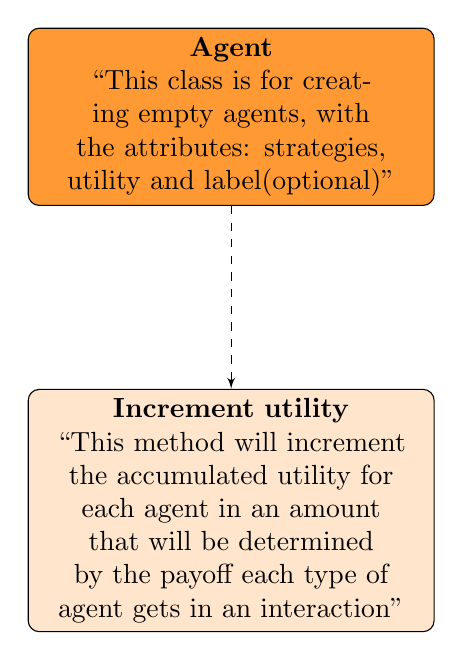
\begin{tikzpicture}
    \node [ageblock] (agent) at (0,0) [draw, fill=orange!80] {\textbf{Agent} \\ 
	``This class is for creating empty agents, with the attributes: strategies, utility and label(optional)''};
    \node [ageblock, below of=agent, node distance=5cm](increment)[draw] {\textbf{Increment utility} \\
	``This method will increment the accumulated utility for each agent in an amount that will be determined by the payoff each 				type of agent gets in an interaction''};
    % Draw edges   
    \path[line,dashed](agent) -- (increment);       

\end{tikzpicture}
\caption{ Diagram of population module.}
\label{fig:diagage}
\end{center}
\end{figure}

\subsection{Environments module}
The environments module for this project is the representation of the environment in which the agents will interact.The environment created is called $\pythoninline{bimatrix\_random}$ $\pythoninline{\_environment}$ and has only two characteristics. It is set to make two agents interact by pairing them randomly and it also sets the rules that these paired agents use to interact. Some of the methods contained in this module make use of the ‘random’ module from python. This module is set to be imported when the environment module is executed. 

$\textbf{Bimatrix\_random\_environment}$ creates a $\pythoninline{class BiMatrixRandomEnv}$, named after the characteristics of the environment of interaction which are that the data is given in the form of a bimatrix and that the agents will interact in a random way. This class has an initialization ( $\pythoninline{\_\_init\_\_}$) method that takes as parameters $\pythoninline{number\_of\_agents}$ and $\pythoninline{bimatrix}$, within the initialization some variables are defined, these variables along with the parameters will now be explained:

\begin{itemize}
\item $\pythoninline{ number\_of\_agents:}$ Input by user, total population of agents regardless of the type of agent(i.e. row agent or column agent).
\item $\pythoninline{bimatrix}$ Input by user, bimatrix of payoffs(can be symmetric or assymetric).
\item $\pythoninline{number\_of\_row\_agents:}$ Result from dividing by “2” the previously input value number\_of\_agents. And gives the number of row agents.
\item $\pythoninline{number\_of\_col\_agents:}$ Result from dividing by “2” the previously input value number\_of\_agents. And gives the number of column agents.
\item $\pythoninline{number\_of\_row\_strategies:}$ Number of strategies that will be available for row agents. Calculated by counting how many rows the bimatrix has.
\item $\pythoninline{number\_of\_col\_strategies:}$ Number of strategies that will be available for column agents. Calculated by counting how many columns the bimatrix has.
\item $\pythoninline{row\_strategies:}$ List containing the available strategies for row agents.
\item $\pythoninline{col\_strategies:}$ List containing the available strategies for column agents.
\end{itemize}

After the initialization, a method $\pythoninline{interact}$ is defined. This method first defines a variable called $\pythoninline{pairs}$ which is assigned to a function $\pythoninline{randomly\_pair\_agents}$ that will be explained later. It also contains a $\pythoninline{``for'' loop}$ this loop within other things contains a variable which is set to a function $\pythoninline{strategies\_to\_utilities}$ which will be explained, variables in the $\textbf{``for'' loop}$ are the following:

\begin{itemize}
\item $\pythoninline{ra}$: Used in the code during for loops instead of $\pythoninline{row\_agents}$.
\item $\pythoninline{ca}$: Used in the code during for loops instead of $\pythoninline{col\_agents}$.
\item $\pythoninline{pairs}$: Variable created to represent the group of paired $\pythoninline{row\_agents}$ with $\pythoninline{col\_agents}$.
\item $\pythoninline{utility}$: Variable used to obtain the utilities resulting from the interaction from each pair of agents ($\textbf{row\_agents and col\_agents}$).
\item $\pythoninline{Agent.increment\_utility}$: The increment utility function is defined in the population model. The structure for in this “for” loop is as follows:
\\ agent.increment\_utility(utility[x]) and what it does is assign the function increment utility to an agent can be $\pythoninline{ra (row\_agent)}$ or$\pythoninline{ ca (col\_agent)}$, the $\pythoninline{utility}$ in parenthesis was assigned in the previous variable, and it is only calling the value with the position x in the list. Given that we only have 2 types of players (we are using a bimatrix) x can be either 0 or 1.
\end{itemize}

Following $\pythoninline{interact}$ the method previously mentioned $\pythoninline{strategies\_to\_utilities}$ is defined. This method is in charge of obtaining the specific pair of utilities (assigned to row and column) from the $\pythoninline{bimatrix}$. It then returns these values to the $\pythoninline{utility}$ variable in the $\pythoninline{interact}$ method and interact uses it to assign the utilities to each agent.

After $\pythoninline{strategies\_to\_utilities}$ the method $\pythoninline{randomly\_pair\_agents}$ is defined. This method is used by $\pythoninline{interact}$ too, and what it does is that the previously created row and column agents that are contained in lists are randomly selected (one of each type) and then paired so they can interact. The following diagram shows in general terms the structure of the bimatrix random environment module:

\begin{figure}[H]
\resizebox{\textwidth}{!}{%
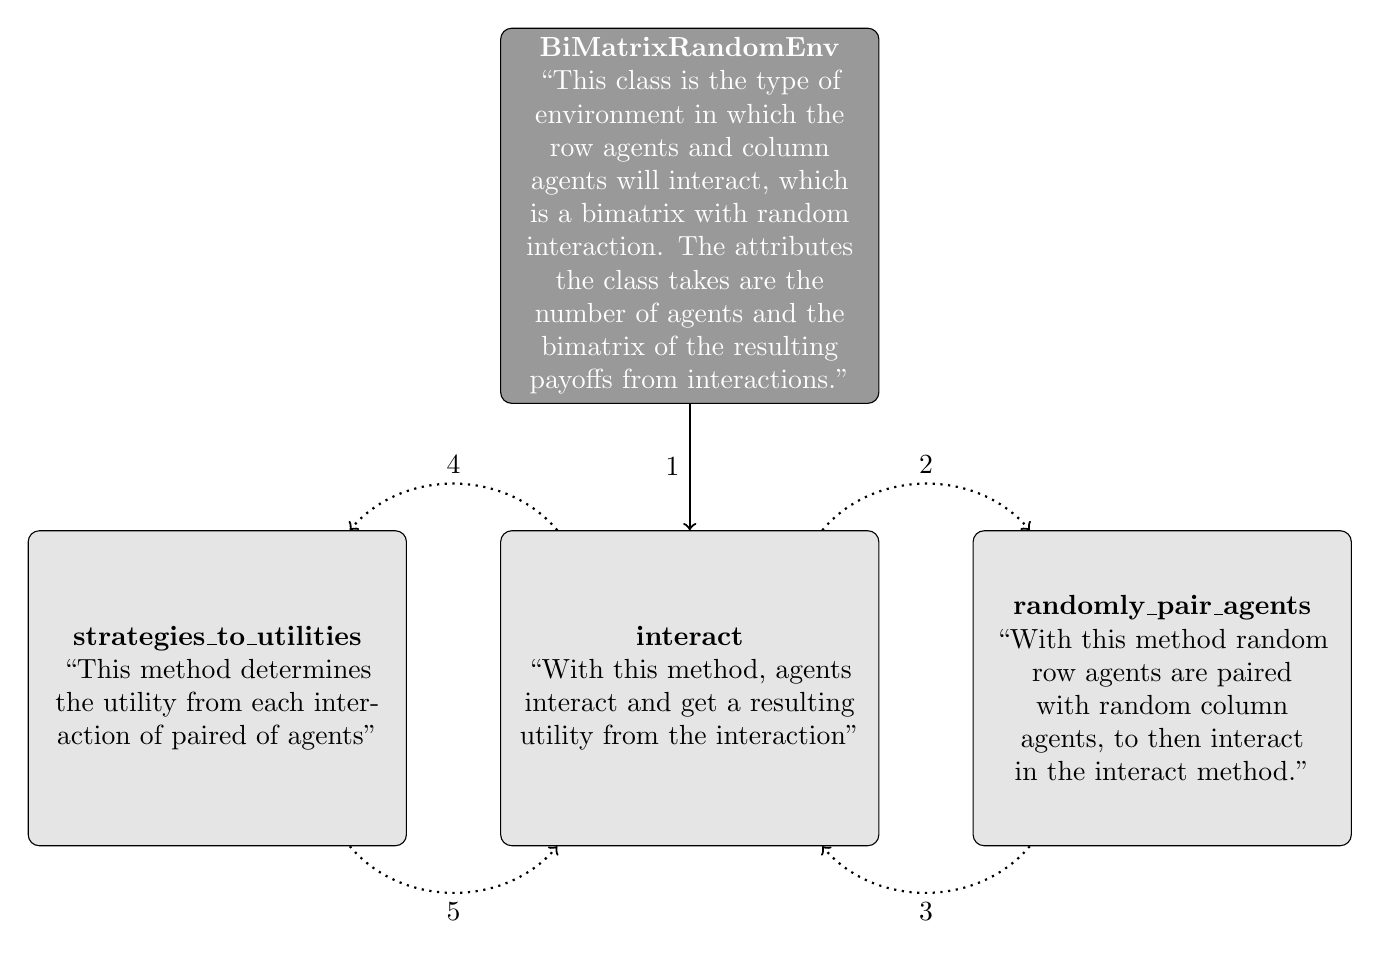
\begin{tikzpicture}[node distance = 2cm, auto]
    \node [envblock, node distance=4cm] (bimatrix) [draw, fill=gray!80,text=white] {\textbf{BiMatrixRandomEnv} \\
    ``This class is the type of environment in which the row agents and column agents will interact, which is a bimatrix with random interaction. The attributes the class takes are the number of agents and the bimatrix of the resulting payoffs from interactions.''};
    \node [envblock, below of=bimatrix, node distance=6cm] (interact) [draw] {\textbf{interact} \\
	``With this method, agents interact and get a resulting utility from the interaction''};
    \node [envblock, left of=interact, node distance=6cm](utilities)[draw] {\textbf{strategies\_to\_utilities} \\
	``This method determines the utility from each interaction of paired of agents''};
    \node [envblock, right of=interact, node distance=6cm] (pairs) [draw] {\textbf{randomly\_pair\_agents} \\
	``With this method random row agents are paired with random column agents, to then interact in the interact method.''};  
    % Draw edges
    \draw [->, thick, black!100] (bimatrix) edge [out=270, in=90] node[left] {1}  (interact);
    \draw [->, thick, dotted, black!100] (interact) edge [out=130, in=50]node[above] {4} (utilities);
    \draw [->, thick,dotted, black!100] (interact) edge [out=50, in=130] node[above] {2} (pairs);
    \draw [->, thick, dotted, black!100] (utilities) edge [out=310, in=230] node[below] {5} (interact);
    \draw [->, thick,dotted, black!100] (pairs) edge [out=230, in=310] node[below] {3} (interact);
 \end{tikzpicture}}
\caption{ Diagram of environments module.}
\label{fig:diagenv}
\end{figure}

\newpage
\subsection{Algorithms module}
The $\textbf{algorithms module}$ is a module that is meant to contain different algorithms by which the created $\textbf{agents}$ from $\textbf{population module}$ will be processed. For this project $\textbf{algorithms module}$ contains a $\textbf{genetic algorithm}$.
The $\textbf{genetic algorithm}$ is named $\textbf{genetic}$ and it creates a $\pythoninline{class Genetic}$. In the initialization ($\pythoninline{\_\_init\_\_}$) takes the following parameters:

\begin{itemize}
	\item $\pythoninline{generations:}$ Are the number of generations (times) the whole code will be run.
	\item $\pythoninline{rounds\_per\_generation:}$ Are the number of times the interaction of the agents will be given within each generation. 
	\item $\pythoninline{death\_rate:}$ Represents the proportion of agents that will be eliminated after each generation has run.
	\item $\pythoninline{mutation\_rate:}$ This parameter is given as a limit for agents with the highest accumulated utility not being reproduced. A $\pythoninline{mutation\_rate}$ value is established and is compared against a $\pythoninline{random.random()}$ number. Every time the $\pythoninline{mutation\_rate}$ is higher than the value given by the $\pythoninline{random.random()}$ a mutation will occur. This comparison occurs every time a new agent is created when all the interactions within a generation have happened. This means that each new agent is passed under this condition. The numbers given by $\pythoninline{random.random()}$ are decimal numbers, which means that the range for $\pythoninline{mutation\_rate}$ should also be in decimal numbers from $\textbf{ 0 to 1}$.
	\item $\pythoninline{exploitation\_rate:}$ Is a variable introduced to determine if the concept of $\textit{exploitation}$ or $\textit{exploration}$ will be used. Where a value of 1 (100$\%$) represents a total exploitation, this means reproducing only the agent with the highest utility for each type of agent ($\pythoninline{row\_agents}$ and $\pythoninline{col\_agents}$) and a value of 0 (0$\%$) is used to consider the whole population of agents.
	\item $\pythoninline{initial\_strategy\_distribution:}$ Is an optional parameter that will allow to the user to introduce the initial proportions of the strategies, meaning what percentage of the population each strategy will be represented by. The distribution will  be introduced as a form of a list within `[ ]' with commas separating the different values. The proportions that are input have to add up to 1 since the number 1 represents 100\% of the population i.e. [0.7, 0.3] added up are equal to 1, this means that the strategy with the first position in the bimatrix will start will be represented by 70\% of the total population of the created agents and the strategy in the second position will be represented by the remaining 30\% of the created agents in the population at the beginning of the simulation. If a particular $\pythoninline{initial\_strategy\_distribution}$ is not needed, the `list' with the proportions does not need to be introduced and the program will automatically set the distribution in almost equal proportions according to the number of strategies.
\end{itemize}

Following the initialization ($\pythoninline{\_\_init\_\_}$), the method $\pythoninline{assign\_strategies}$ is found. This method takes parameters $\textbf{agents}$, which according to the type of agent in turn will be represented by $\pythoninline{row\_agents}$ or $\pythoninline{col\_agents}$  and the parameter $\pythoninline{agents\_strategies}$, also which according to the type of agent in turn will be represented by $\pythoninline{row\_strategies}$ or $\pythoninline{col\_strategies}$. This method is used after the different types of agents are created in the $\pythoninline{initialization}$ of the $\pythoninline{class BiMatrixRandomEnv}$ of the module $\pythoninline{environments}$. The $\pythoninline{assign\_strategies}$ method assigns a random strategy for each agent according to the strategies available given their type through a $\textbf{``for'' loop}$ and random.choice $\pythoninline{(agents\_strategies)}$ this random choice selects from the $\pythoninline{row\_strategies}$ or $\pythoninline{col\_strategies}$ randomly according to the type of agent.

After the ($\pythoninline{assign\_strategies}$) method in the code, the method alternative method in case a specific initial distribution is required  $\pythoninline{assign\_strategies\_initial\_distribution}$ is found. This method takes parameters $\textbf{agents}$, which according to the type of agent in turn will be represented by $\pythoninline{row\_agents}$ or $\pythoninline{col\_agents}$, the parameter $\pythoninline{agents\_strategies}$, also which according to the type of agent in turn will be represented by $\pythoninline{row\_strategies}$ or $\pythoninline{col\_strategies}$, the parameter $\pythoninline{number\_of\_agents}$ which is the total number of agents in the simulation, and the parameter $\pythoninline{agent\_initial}$ $\pythoninline{\_distribution}$ which is a list that holds the proportions in which the strategies are required to appear at the beginning of the simulation. This method has the same purpose as $\pythoninline{assign\_strategies}$ with the only difference that when selecting an initial strategy distribution the program will create the exact proportion of agents strategies that is required. After creating a list of agents with strategies in the proportions required it will be found that the agents were created in order, to continue with the random environment required the method $\pythoninline{random.shuffle}$ from the module $\pythoninline{random}$ is used. This way the order of the agents will not be a specific when interacting with each other in the second generation.

After the $\pythoninline{assign\_strategies}$ method, comes a method named $\pythoninline{kill\_agents}$. This method takes as parameters $\pythoninline{agents}$, $\pythoninline{number\_of\_agents}$, $\pythoninline{number\_of\_x\_agents}$, and                       $\pythoninline{agents\_}$ $\pythoninline{strategies}$. In this method a variable $\pythoninline{number\_of\_deaths\_per\_generation}$ is created, which determines the number of agents that will be eliminated for each type of agent group ($\pythoninline{row\_agents}$ or $\pythoninline{ col\_agents}$) it does so by taking the integer value from the product of the multiplication of the variables $\pythoninline{death\_rate}$ * $\pythoninline{number\_of\_x\_agents}$(this last variable represents the total number of row\_agents or col\_agents).  The value $\pythoninline{number\_of\_deaths}$ $\pythoninline{\_per\_generation}$ is used in a $\textbf{``while'' loop}$ to eliminate the agents while the condition is not satisfied. Within the ``while'' loop the agents ($\pythoninline{row\_agents}$ or $\pythoninline{col\_agents)}$  are sorted according to their accumulated $\pythoninline{utility}$ from smallest to highest and the one with the lowest accumulated $\pythoninline{utility}$ is deleted from the list of the corresponding type of agents.

After the method $\pythoninline{kill\_agents}$ comes the method $\pythoninline{reproduce\_agents}$. This method takes as parameters $\pythoninline{agents}$, $\pythoninline{number\_of\_agents}$, $\pythoninline{number\_of\_x\_agents}$, and $\pythoninline{agents\_strategies}$. A variable $\pythoninline{choice}$ is created by taking the integer value of ($\pythoninline{((number\_of\_agents / 2) }$ * $\pythoninline{(exploitation\_rate - 1) + 0.05) -1}$) this value is used within the ``while'' loop that follows. The ``while'' loop used in this method works while the existing number of row or col agents is less than the number of row or col agents created at the beginning of the simulation. Within this loop, the agents are sorted according to their accumulated $\pythoninline{utility}$ values from low to high, and a $\pythoninline{copy.deepcopy}$  function is used to create a copy of an agents chosen with $\pythoninline{random.choice(agents[choice:])}$ where the variable $\pythoninline{choice}$ will indicate the start of the range of agents that can be chosen within the list of agents. After this within the same loop and ``if'' statement is presented which condition is that if the $\pythoninline{mutation\_rate}$ value is greater than a $\pythoninline{random.random()}$ number, the agent that will be reproduced can be any agent (row or col agent) with any value of accumulated $\pythoninline{utility}$ except for the agent (row or col agent) with the highest accumulated $\pythoninline{utility}$  value of that generation. The following diagram shows the general structure of the genetic algorithm module:

\begin{figure}[H]
\resizebox{\textwidth}{!}{%
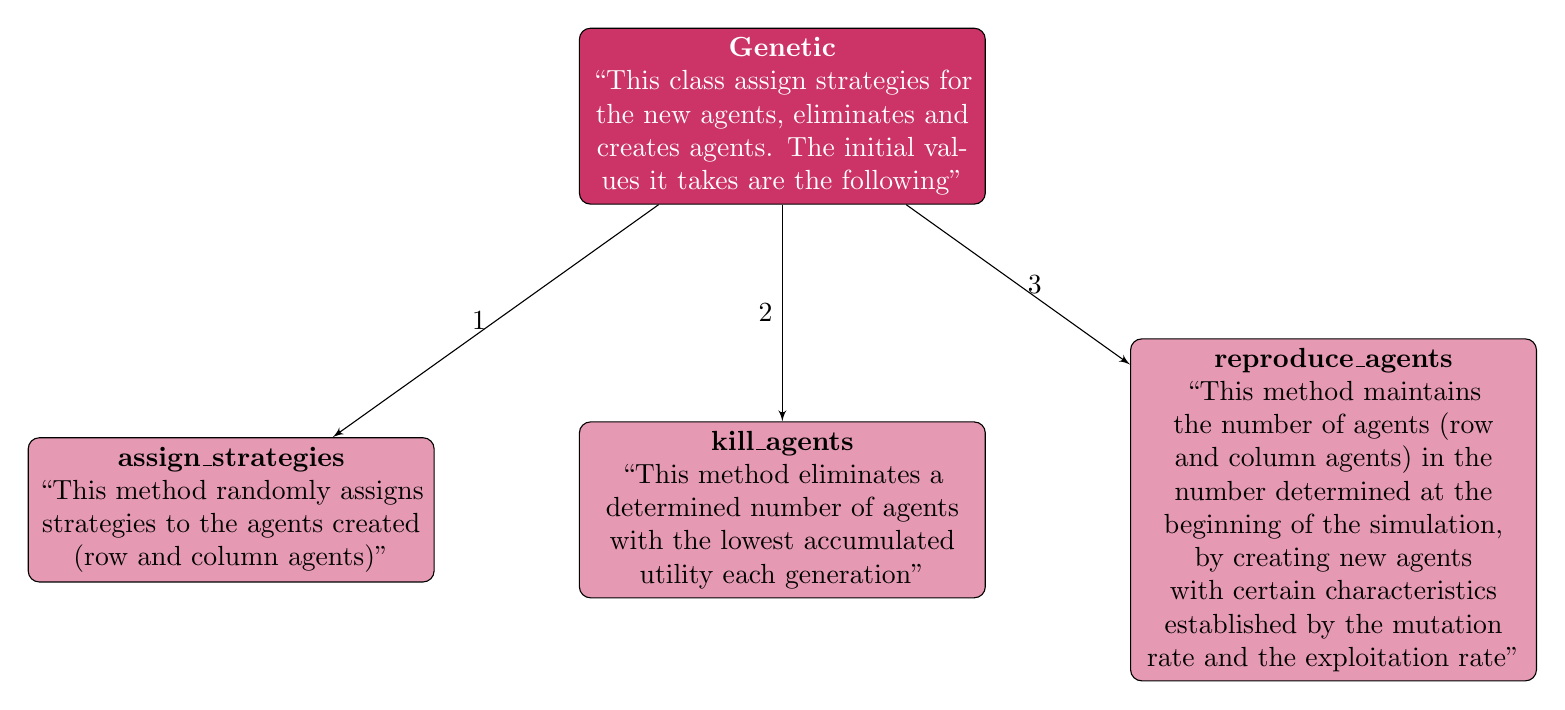
\begin{tikzpicture}
    \node [algblock] (genetic) at (0,0) [draw, fill=purple!80, text=white] {\textbf{Genetic} \\ 
	``This class assign strategies for the new agents, eliminates and creates agents. The initial values it takes are the following''};
    \node [algblock, below of=genetic, node distance=5cm](kill)[draw] {\textbf{kill\_agents} \\
	``This method eliminates a determined number of agents with the lowest accumulated utility each generation''};
    \node [algblock, right of=kill, node distance=7cm](repro)[draw] {\textbf{reproduce\_agents} \\
	``This method maintains the number of agents (row and column agents) in the number determined at the beginning of the 			simulation, by creating new agents with certain characteristics established by the mutation rate and the exploitation rate''};
    \node [algblock, left of=kill, node distance=7cm](assign)[draw] {\textbf{assign\_strategies} \\
	``This method randomly assigns strategies to the agents created (row and column agents)''};
    % Draw edges   
    \path[line](genetic) edge         node[left] {1} (assign);
    \path[line](genetic) edge         node[left]{2} (kill);
    \path[line](genetic) edge         node[right] {3} (repro);         
\end{tikzpicture}}
\caption{Diagram of algorithms module.}
\label{fig:diagalg}
\end{figure}



\subsection{Simulation module}
The $\textbf{simulation module}$ is a module that is makes all the other modules interact with each other. For this project $\textbf{simulation module}$ is named $\pythoninline{simulation}$  and it creates a $\pythoninline{class Simulation}$. In the initialization ($\pythoninline{\_\_init\_\_}$) takes the parameters used in the other modules in addition to another parameter named $\pythoninline{tog}$ which stands for ``type of game''. There are 7 predetermined games within the code, which can be selected by typing the correct value of $\pythoninline{tog}$. $\pythoninline{tog}$ and the other parameters taken by the class $\pythoninline{Simulation}$ have the following characteristics:

\begin{itemize}
	\item $\pythoninline{tog:}$ Stands for ``type of game'' and it serves to pick one of the available choices of bimatrix that have been coded in. The values that can be selected have to go between single quotation marks and are the following: $\pythoninline{`pd'}$ an example of prisoner's dilemma, $\pythoninline{`psr'}$ an example of the game paper-scissors-rock, $\pythoninline{`mp'}$ an example of matching pennies, $\pythoninline{`bos'}$ an example of battle of sexes game, $\pythoninline{`hd'}$, $\pythoninline{`sh'}$ an example of stag hunt game, $\pythoninline{`cs'}$ an example of choosing sides game and $\pythoninline{`axl'}$ an example emulating the first tournament from Robert Axelrod with 8 out of the 14 original strategies. This strategies are taken from the axelrod package available for python and with the following strategies: $\textit{Tit for Tat}$, $\textit{Grofman}$, $\textit{Shubik}$, $\textit{Grudger}$, $\textit{Davis}$, $\textit{Feld}$, $\textit{Joss}$ and $\textit{Tullock}$.
	\item$\pythoninline{na:}$ Stands for the value of $\pythoninline{number\_of\_agents}$ explained in the $\pythoninline{bimatrix\_random}$$\pythoninline{\_environment}$ module.
	\item $\pythoninline{ge:}$ Stands for the value of $\pythoninline{generations}$ explained in the $\pythoninline{genetic}$ algorithm module. And is the number of generations (times) the whole code will be run.
	\item $\pythoninline{rpg:}$ Stands for the value of $\pythoninline{rounds\_per\_generation}$ explained in the $\pythoninline{genetic}$  algorithm module. Is the number of times the interaction of the agents will be given within each generation. 
	\item $\pythoninline{dr:}$ Stands for $\pythoninline{death\_rate}$ explained in the $\pythoninline{genetic}$ algorithm module. And represents the proportion of agents that will be eliminated after each generation has run.
	\item $\pythoninline{mr:}$ Stands for $\pythoninline{mutation\_rate}$ explained in the $\pythoninline{genetic}$ algorithm module. And this parameter is given as a limit for agents with the highest accumulated utility not being reproduced. A $\pythoninline{mutation\_rate}$ value is established and is compared against a $\pythoninline{random.random()}$ number. Every time the $\pythoninline{mutation\_rate}$ is higher than the value given by the $\pythoninline{random.random()}$ a mutation will occur. This comparison occurs every time a new agent is created when all the interactions within a generation have happened. This means that each new agent is passed under this condition. The numbers given by $\pythoninline{random.random()}$ are decimal numbers, which means that the range for $\pythoninline{mutation\_rate}$ should also be in decimal numbers from $\textbf{ 0 to 1}$.
	\item $\textbf{er:}$ Stands for $\pythoninline{exploitation\_rate}$ explained in the $\textbf{genetic}$ algorithm module. And it is a variable introduced to determine if the concept of $\textit{exploitation}$ or $\textit{exploration}$ will be used. Where a value of 1 (100$\%$) represents a total exploitation, this means reproducing only the agent with the highest utility for each type of agent ($\pythoninline{row\_agents}$ $\pythoninline{col\_agents}$) and a value of 0 (0$\%$) is used to consider the whole population of agents.
	\item $\textbf{isd:}$ Stands for $\pythoninline{initial\_strategy\_distribution}$ explained in the $\textbf{genetic}$ algorithm module. It takes a list of decimal numbers which should add up to 1, each value representing the proportion for each strategy available in the $\pythoninline{bimatrix}$. In here is where the user inputs the initial distribution desired for the strategies. At the beginning of the simulation this value will be used by the instance created from the $\pythoninline{class Genetic}$ from the genetic module to assign the initial strategies to each agent.
\end{itemize}

In the initialization ($\pythoninline{\_\_init\_\_}$) method an instance of the $\pythoninline{class Genetic}$ from the genetic module is created, an instance for the $\pythoninline{class Agents}$ from the population module is created also and when selecting the $\pythoninline{tog}$ value, an instance of the $\pythoninline{class}$ $\pythoninline{BiMatrixRandomEnv}$ from the environment module is created. After the instances are created within the initialization method, the functions $\pythoninline{ga.assign\_strategies()}$ or $\pythoninline{ga.assign\_strategies}$$\pythoninline{\_initial\_distribution()}$ from the genetic algorithm module is used to assign the values for the strategies for each type of agent ($\pythoninline{row\_agents}$ and $\pythoninline{col\_agents}$) that have been created through the instance of the module environment can be used, the methods are conditioned under an if statement which checks if an initial distribution was introduced or not. After three lists with the names $\pythoninline{row\_accumulated\_strategies}$, $\pythoninline{col\_acummulated\_strategies}$ and $\pythoninline{strategies\_history}$ are created respectively and the purpose for each list is the following:

\begin{itemize}
	\item$\pythoninline{row\_accumulated\_strategies}$: Creates a list, that within itself contains a certain number of individual lists according to the length of $\pythoninline{row\_strategies}$ which is the number of strategies available for the $\pythoninline{row\_agents}$ obtained from the module environment.
	\item$\pythoninline{col\_accumulated\_strategies}$: Creates a list, that within itself contains a certain number of individual lists according to the length of $\pythoninline{col\_strategies}$ which is the number of strategies available for the $\pythoninline{col\_agents}$ obtained from the module environment.
	\item$\pythoninline{strategies\_history}$: Creates a list, that within itself contains a certain number of individual lists according to the length of $\pythoninline{row\_strategies}$ if $\pythoninline{row\_strategies}$ $\geq$ $\pythoninline{col\_strategies}$, else it creates a number of lists according to the number of $\pythoninline{col\_strategies}$. This list will help to create the stack plot, and what it does is it stores the total numbers of each type of strategy (not taking in account the type of agent) in a list that is generated each generation and all these lists created per generation are contained within a list that helps create the stack plot.

\end{itemize}

After the initialization method has created the different instances from the other modules, a method with the name $\pythoninline{run(plot=False, stack=False)}$ is presented. This method is used to start running the whole simulation (all the modules). The method takes an attribute $\pythoninline{plot}$ which is set by default as $\pythoninline{False}$ and an attribute $\pythoninline{stack}$ which is also set by default as $\pythoninline{False}$, if using the method $\pythoninline{run(plot=True, stack=True)}$, the simulation will plot the results from each generation in a graph and at the end of the simulation will produce a stack plot representing how the number of agents for each strategy behaved. The graph and stack plot are produced with the module $\pythoninline{matplotlib}$ from python and the functions used are $\textbf{pyplot and cm(color map)}$. The graph is set in interactive mode by the function $\pythoninline{ion( )}$. The limits for the graph's y axis are set $\pythoninline{ylim(0, 1)}$ and for the stack plot the y axis shows the total number of agents, the limit for the x axis for graph and stack plot are the number of $\pythoninline{generations}$. The x axis for both is labeled $\pythoninline{xlabel(``Generations")}$ and the y axis is labeled $\pythoninline{ylabel(``Probability'')}$ for graphs and $\pythoninline{ylabel(``Agents'')}$ for stack plots. For the coloring the lines representing the different strategies for each type of agents in the graphs color map method from mathplotlib is used, for the $\pythoninline{row\_accumulated\_strategies[ ]}$ the color map copper is used and for the $\pythoninline{col\_accumulated\_strategies[ ]}$ the color map winter is used, how these $\pythoninline{accumulated}$ $\pythoninline{\_strategies}$ values were obtained for graphs will be explained later, the thing to know about them is that each of them represent the proportion within a type of agent that is using a certain strategy. The graph indicates how the population of the different types of agents with strategies varied through time, the value of interest from this is the strategy the types of agents are using. While the stack plot does not make a distinction between types of agents and it shoes the total number of each type of strategy in the total population through the whole simulation.

After the code for creating the graph a function $\pythoninline{generations\_passing( )}$ is presented, this function takes attributes $\pythoninline{generations}$, $\pythoninline{rounds\_per\_generation}$, $\pythoninline{number\_of\_agents}$, $\pythoninline{row\_agents}$, $\pythoninline{col\_agents}$, and $\pythoninline{plot}$ and takes us to the next method.

After the $\pythoninline{run}$ method, there is a method $\pythoninline{generations\_passing}$ that takes attributes $\pythoninline{generations}$,  $\pythoninline{row\_agents}$, $\pythoninline{col\_agents}$, $\pythoninline{number\_of\_agents}$, $\pythoninline{ plot}$. In this method there is a ``for'' loop that loops until the $\pythoninline{generations}$ value is reached, within this loop exist two other ``for'' loops.
 he first one loops around the $\pythoninline{row\_agents}$ and  $\pythoninline{col\_agents}$ setting for each agent  the $\pythoninline{utility}$ value to 0. 
The second ``for'' loop loops according to the $\pythoninline{number\_of\_rounds}$ chosen at the beginning of the simulation. Within this loop we find the function $\pythoninline{interact( )}$ from the module environment, explained before, which in general terms makes the $\pythoninline{row\_agents}$ and $\pythoninline{col\_agents}$ interact with each other and as a result obtains the payoff for each type of agent and an attributed $\pythoninline{utility}$. The loop from the rounds causes this process to repeat several times and when the last round is played all the different agents have an accumulated utility product of the repeated interactions.
When the second loop concludes a function $\pythoninline{distributions( )}$ follows. This function is for the method $\pythoninline{distributions}$ that takes attributes $\pythoninline{number\_of\_agents}$, $\pythoninline{ row\_agents}$, $\pythoninline{col\_agents}$, $\pythoninline{row\_strategies}$, $\pythoninline{col\_strategies}$, and$\pythoninline{ plot}$.

Before the method $\pythoninline{distributions}$ there are two methods, the first is $\pythoninline{proportion}$ $\pythoninline{\_classified\_strategies}$ that takes attributes $\pythoninline{agents}$ and $\pythoninline{strategies}$. This method will do some calculations when the code is using the method $\pythoninline{distributions}$.   The method first creates a varibale $\pythoninline{frequency\_per\_strategy\_per\_agent}$ with an empty list. Then it has a ``main'' ``for'' loop that loops around the variable $\pythoninline{strategies}$ (this variable can be $\pythoninline{row\_strategies}$ or $\pythoninline{col\_strategies}$ according to which values are being used) of the $\pythoninline{agent}$ in turn and appends a value of 0 to the list. Then an ``secondary'' loop is contained within the previous loop of $\pythoninline{strategies}$, this loops around the agents in turn (can be $\pythoninline{row\_agents}$ or $\pythoninline{col\_agents}$) and contains an ``if'' statement, which conditions if  the strategy from the $\pythoninline{agent}$ in turn is equal to the counter in the ``main'' loop for ($\pythoninline{strategies}$) the last value of the list $\pythoninline{frequency\_per\_strategy\_per\_agent}$ will increment by 1. When both loops finish the function returns a list with all the values that are contained in the $\pythoninline{frequency\_per\_strategy\_per\_agent}$, each of those values are devided by the number agents. This values are the proportion that strategy represents in the type of agents in turn. It is important to note that the variable $\pythoninline{agents}$ taken by this function can be either $\pythoninline{row\_agents}$ or $\pythoninline{col\_agents}$   and the variable $\pythoninline{strategies}$ can be either $\pythoninline{row\_strategies}$ or $\pythoninline{col\_strategies}$. 

The second method before $\pythoninline{distributions}$ method is $\pythoninline{total\_classified\_strategies}$ that takes attributes $\pythoninline{row\_agents}$, $\pythoninline{row\_strategies}$, $\pythoninline{col\_agents}$ and $\pythoninline{col\_strategies}$. This method will do some calculations when the code is using the method $\pythoninline{distributions}$ for getting the total number of each type of strategy.   The method first creates a varibale $\pythoninline{frequency\_per\_strategy\_for\_sum}$ with an empty list. Then it has a ``main'' ``for'' loop that loops around the variable $\pythoninline{row\_strategies}$ and appends a value of 0 to the list. Then an ``secondary'' loop is contained within the previous loop of $\pythoninline{row\_strategies}$, this loops around the $\pythoninline{row\_agents}$ and contains an ``if'' statement, which conditions if  the strategy from the $\pythoninline{row\_agents}$ is equal to the counter in the ``main'' loop for ($\pythoninline{row\_strategies}$) the last value of the list $\pythoninline{frequency\_per\_strategy\_for\_sum}$ will increment by 1. When both loops finish the function returns a list with all the values that are contained in the $\pythoninline{frequency\_per\_strategy\_for\_sum}$ and repeats the same process for $\pythoninline{col\_agents}$ with their corresponding $\pythoninline{col\_strategies}$. This values are accumulated in strategies, so there is no distinction between the type of agents only between type of strategy regardless if it is from $\pythoninline{row\_agents}$ or $\pythoninline{col\_agents}$. It is important to mention that the loops for both types of agents are conditioned with an `if' statement, where if the $\pythoninline{row\_agents}$ have more or equal types of strategies $\pythoninline{row\_strategies}$ than $\pythoninline{col\_agents}$the first for loop to start producing the list in the variable $\pythoninline{frequency\_per\_strategy\_for\_sum}$ will be the $\pythoninline{row\_agents}$' loop, else if the $\pythoninline{col\_agents}$ have more types of strategies $\pythoninline{col\_strategies}$ than $\pythoninline{row\_agents}$, the $\pythoninline{col\_agents}$ loop will go first. This conditional statement is used in case that there is a non symmetric type of game where $\pythoninline{col\_agents}$ have a higher number of $\pythoninline{col\_strategies}$ than $\pythoninline{row\_agents}$ of its own type of strategies.

When the method $\pythoninline{distributions}$ starts first it creates a variable $\pythoninline{row\_strategies}$ $\pythoninline{\_distribution}$ this variable contains a function $\pythoninline{proportion\_classified\_strategies( )}$ that takes as attributes $\pythoninline{row\_agents}$ and $\pythoninline{row\_strategies}$. And then has a ``for'' loop which loops around the number of  $\pythoninline{row\_strategies}$ and appends into the list created at the initialization $\pythoninline{row\_accumulated\_strategies}$ the resulting value from the $\pythoninline{row\_strategies\_distribution}$. According to which strategy it belongs, it appends the value to the corresponding list. 
Then the method creates second variable which has the same process as the previous, but with $\pythoninline{col\_agents}$. The variable it creates is $\pythoninline{col\_strategies\_distribution}$ this variable contains a function $\pythoninline{proportion\_classified}$ $\pythoninline{\_strategies( )}$ that takes as attributes $\pythoninline{col\_agents}$ and $\pythoninline{col\_strategies}$. Then has a ``for'' loop which loops around the number of  $\pythoninline{col\_strategies}$ and appends into the list created at the initialization $\pythoninline{col\_accumulated\_strategies}$ the resulting value from the $\pythoninline{col\_strategies\_distribution}$. According to which strategy it belongs, it appends the value to the corresponding list.  Then a third variable  $\pythoninline{total\_strategies\_per\_generation}$ is created. This variable contains a function $\pythoninline{total\_classified\_strategies( )}$ that takes as attributes $\pythoninline{row\_agents}$, $\pythoninline{row\_strategies}$, $\pythoninline{col\_agents}$ and $\pythoninline{col\_strategies}$. And then has a ``for'' loop which loops around the number of lists contained in  $\pythoninline{strategies\_history}$ and appends into the list created at the initialization $\pythoninline{strategies\_history}$ the resulting value from the $\pythoninline{total\_strategies\_per\_generation}$. According to which generation it belongs, it appends the value to the corresponding list. After these three variables, and the append of $\pythoninline{row\_strategies\_distribution[  ]}$ to $\pythoninline{row\_accumulated\_strategies[  ]}$ and $\pythoninline{col\_strategies\_distribution[  ]}$ to $\pythoninline{col\_accumulated\_strategies[  ]}$ is finished. The method then $\textbf{prints}$ four lines, the first one contains the following text $\textit{``Row players'}$ $\pythoninline{strategy distribution:"}$, the second line prints the list $\pythoninline{row\_strategies\_distribution}$, the third line prints the text $\textit{``Column players' strategy distribution:"}$, and the fourth line prints the list $\pythoninline{col\_strategies\_distribution}$. 
After these lines come two lines, each with the function $\pythoninline{kill\_agents( )}$ from the genetic algorithm module. One of which is for eliminating $\pythoninline{row\_agents}$ and the other for eliminating $\pythoninline{col\_agents}$.  
Then we have other two lines, each with the function $\pythoninline{reproduce\_agents( )}$ from the genetic algorithm module. One to create the $\pythoninline{row\_agents}$ that were previously eliminated until reaching the required number of $\pythoninline{row\_agents}$ and the other to create $\pythoninline{col\_agents}$ until reaching the required number of $\pythoninline{col\_agents}$. 
After the last $\pythoninline{reproduce\_agents( )}$ function, a code to update the graph is run (if it was chosen to graph at the beginning of the simulation). 
The whole cycle is repeated until the simulation reaches the number of $\pythoninline{generations}$ that was established at the beginning. The following diagram shows the general structure of the simulation module:

\begin{figure}[H]
\resizebox{\textwidth}{!}{%
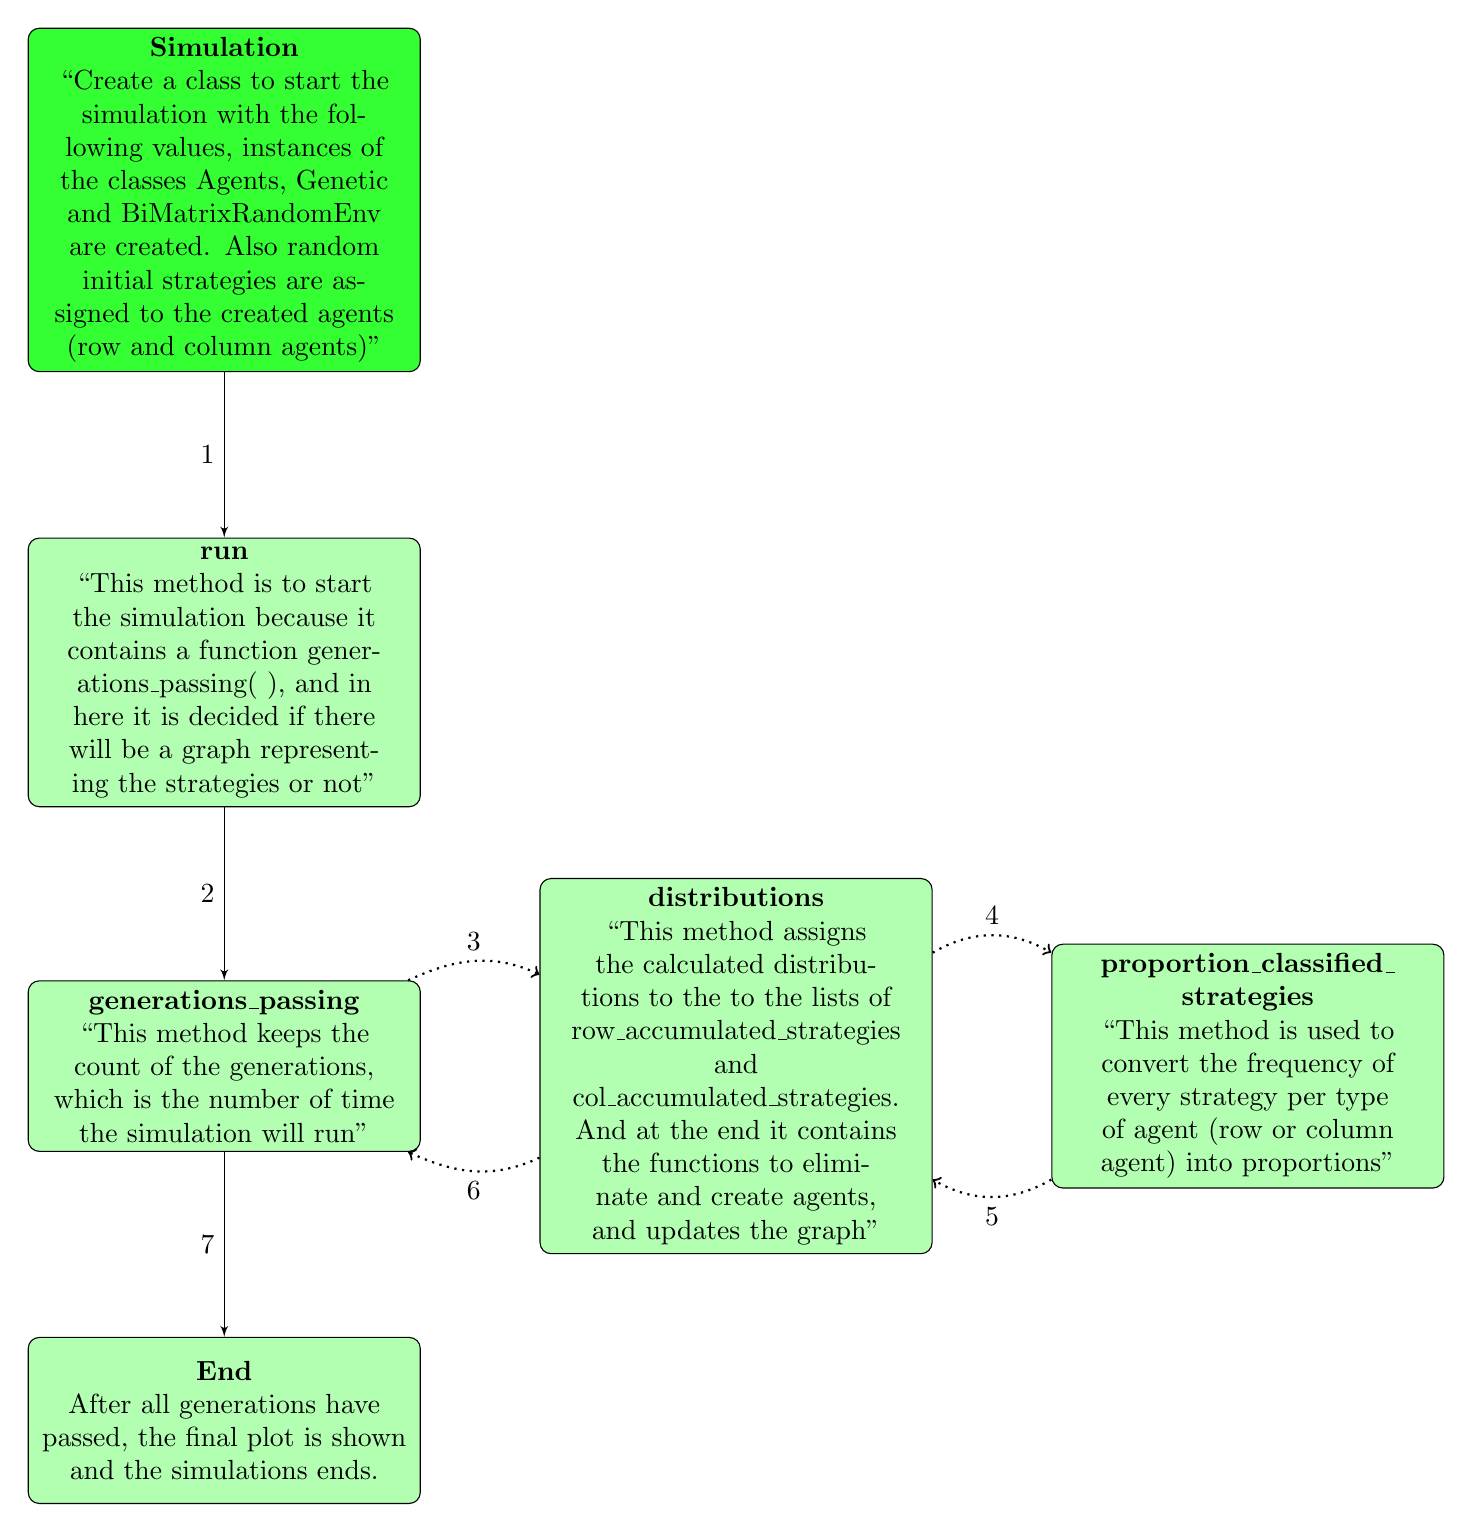
\begin{tikzpicture}[node distance = 2cm, auto]
    % Place nodes
    \node [simblock, fill=green!80] (sim) {\textbf{Simulation} \\
	``Create a class to start the simulation with the following values, instances of the classes Agents, Genetic and 					BiMatrixRandomEnv are created. Also random initial strategies are assigned to the created agents (row and column agents)''};
    \node [simblock, below of=sim, node distance=6cm] (run) {\textbf{run} \\
	``This method is to start the simulation because it contains a function generations\_passing( ), and in here it is decided if there 		will be a graph representing the strategies or not''};
    \node [simblock, below of=run, node distance=5cm] (generations) {\textbf{generations\_passing} \\
	``This method keeps the count of the generations, which is the number of time the simulation will run''};
    \node [simblock, right of=generations, node distance=6.5cm] (distributions) {\textbf{distributions}\\
	``This method assigns the calculated distributions to the to the lists of row\_accumulated\_strategies and 						col\_accumulated\_strategies. And at the end it contains the functions to eliminate and create agents, and updates the 			graph''};
    \node [simblock, right of=distributions, node distance=6.5cm] (proportion) 											{\textbf{proportion\_}\textbf{classified\_} \\ 
	\textbf{strategies} \\
	``This method is used to convert the frequency of every strategy per type of agent (row or column agent) into proportions''};
    \node [simblock, below of=generations, node distance=4.5cm] (end) {\textbf{End} \\
	After all generations have passed, the final plot is shown and the simulations ends.};
    % Draw edges
    \path [line] (sim) -- node[left] {1}  (run);
    \path [line] (run) -- node[left] {2}  (generations);
    \draw [->, thick, dotted, black!100] (generations) edge [out=25, in=155] node[above] {3}  (distributions);
    \draw [->, thick, dotted, black!100] (distributions) edge [out=205, in=335] node[below] {6}  (generations);
    \draw [->, thick, dotted, black!100] (distributions) edge [out=30, in=150] node[above] {4}  (proportion);
    \draw [->, thick, dotted, black!100] (proportion) edge [out=210, in=330] node[below] {5}  (distributions);
    \path [line] (generations) -- node[left] {7} (end);
\end{tikzpicture}}
\caption{Diagram of simulation module.}
\label{fig:diagsim}
\end{figure}


\newpage
\subsection{Overall interaction view}
Now we will have a general overview of how an actual simulation runs. Simulation contains the messages for all the other modules and with this it gives the sequence in which the modules work basically following the steps below:

\begin{itemize}
   \item $\textbf{1. }$ Create agents without a strategy, and with a utility equal to 0 according to the initial number of agents and the given initial distribution. If no initial distribution is entered it will create agents in equal proportions. 
   \item $\textbf{2. }$Then a random strategy is assigned according to the available strategies from the payoff matrix.
   \item $\textbf{3. }$Then the different agent strategies interact, and accumulate a utility. Each interaction is equivalent to a round, so the interactions are repeated according to the number of rounds established at the beginning of the simulation.
   \item $\textbf{4. }$The proportions of the agents present in the population are calculated to be plotted.
   \item $\textbf{5. }$Agents with low utilities are eliminated according to the death rate, since a constant size of population is desired  the same number of agents that were eliminated are created. The new agents are created according to the mutation rate and exploitation rate established at the beginning of the simulation. With low mutation rate and high exploitation rate the agents with highest utility are more likely to be reproduced, this means the new agents will have the same strategy as the agents with highest utility.
   \item $\textbf{6. }$Points 2, 3, 4 and 5 describe the sequence of the code for each generation. And will be repeated according to the number of generations established at the beginning of the simulation.
   \item $\textbf{7. }$After the iteration through the number of generations has finished, the final plot describing the behaviour of the strategies and a stackplot representing the proportions of the strategies in the populations are presented.
   \item $\textbf{8. }$The simulation ends.
\end{itemize}

The following diagram represents in a graphic way how the modules interact: 

\begin{figure}[H]
\resizebox{\textwidth}{!}{%
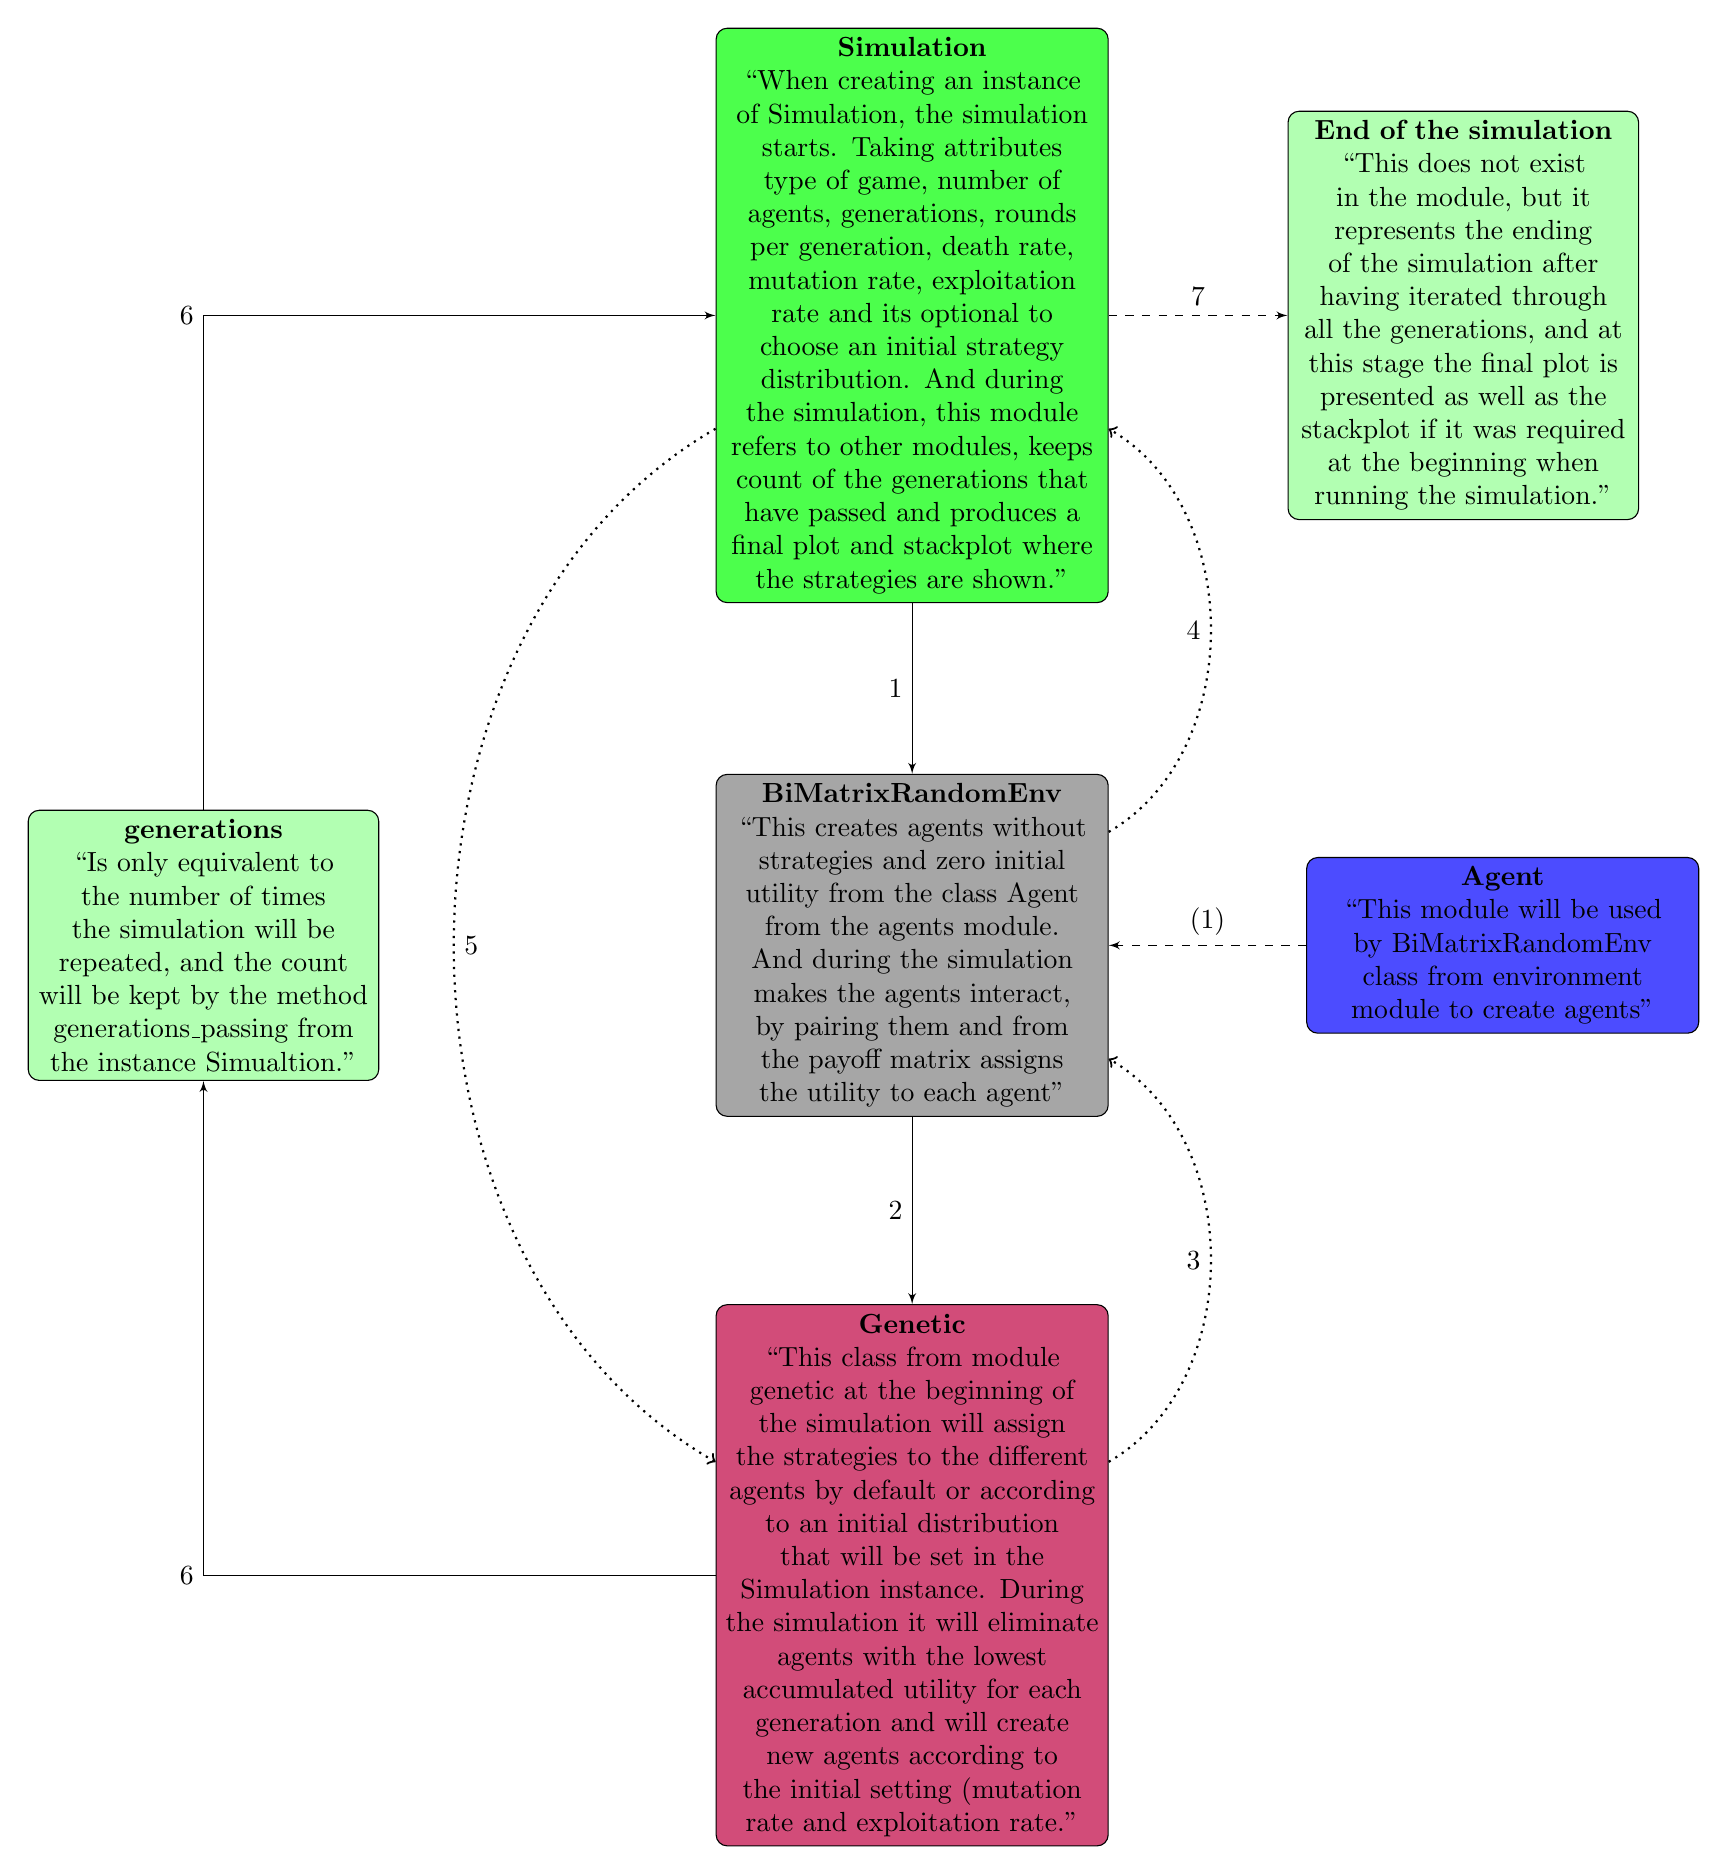
\begin{tikzpicture}
    \node [simblock] (simulation) at (0,0) [draw, fill=green!70] {\textbf{Simulation} \\
	``When creating an instance of Simulation, the simulation starts. Taking attributes type of game, number of agents, 				generations, rounds per generation, death rate, mutation rate, exploitation rate and its optional to choose an initial strategy 			distribution. And during the simulation, this module refers to other modules, keeps count of the generations that have passed 			and produces a final plot and stackplot where the strategies are shown.''};
    \node [simblock, below of=simulation, node distance=8cm](bimatrix)[draw, fill=gray!70] {\textbf{BiMatrixRandomEnv} \\
	``This creates agents without strategies and zero initial utility from the class Agent from the agents module. And during the 			simulation makes the agents interact, by pairing them and from the payoff matrix assigns the utility to each agent''}; 
    \node [simblock, right of=bimatrix, node distance=7.5cm] (agents)[draw, fill=blue!70] {\textbf{Agent} \\
	``This module will be used by BiMatrixRandomEnv class from environment module to create agents''};
    \node [simblock, below of=bimatrix, node distance=8cm](genetic) [draw, fill=purple!70] {\textbf{Genetic} \\ 
	``This class from module genetic at the beginning of the simulation will assign the strategies to the different agents by default 		or according to an initial distribution that will be set in the Simulation instance. During the simulation it will eliminate agents with 			the lowest accumulated utility for each generation and will create new agents according to the initial setting (mutation rate and 	exploitation rate.''};
    \node [geneblock, left of=bimatrix, node distance=9cm](generations) [draw] {\textbf{generations}\\ 
	``Is only equivalent to the number of times the simulation will be repeated, and the count will be kept by the method 				generations\_passing from the instance Simualtion.''};   
    \node [geneblock, right of=simulation, node distance=7cm](end) [draw] {\textbf{End of the simulation}\\ 
	``This does not exist in the module, but it represents the ending of the simulation after having iterated through all the 				generations, and at this stage the final plot is presented as well as the stackplot if it was required at the beginning when 			running the simulation.''};   

    % Draw edges 
    \path [line] (simulation) --  node[left] {1} (bimatrix);
    \path [line] (bimatrix) -- node[left] {2}  (genetic);
    \path [line, dashed] (agents) --  node[above] {(1)}  (bimatrix);
    \draw [->, thick, dotted, black!100] (genetic) edge [out=30, in=330] node[left] {3}  (bimatrix);
   \draw [->, thick, dotted, black!100] (bimatrix) edge [out=30, in=330] node[left] {4}  (simulation);
    \draw [->, thick, dotted, black!100] (simulation) edge [out=210, in=150] node[right] {5}  (genetic);
    \path [line] (genetic) -| node[left] {6}  (generations);
    \path [line] (generations) |-  node[left] {6}  (simulation);
    \path [line, dashed] (simulation) --  node[above] {7}  (end);
\end{tikzpicture}}
\caption{Diagram interaction of modules.}
\label{fig:diagoverall}
\end{figure}



\chapter{Application of the code}
\label{ch:codeapp}
In this chapter the runs of the program will be discussed. What was consider when running a simulation. An explanation of what games were simulated, and of the results against the known techniques to indicate how the program outputs our expected results when running it with known classic game theory games. A comparison of the results given by the  library 'Axelrod' from python with results from this code 'Ablearn'.

\section{How the simulation was built.}
After building the code the objective is to determine if the program gives us the expected results. It is  known that an evolutionary stable strategy is a strategy that survives through time. And as it was mentioned before there are certain conditions that can  be verified in order to identify and evolutionary stable strategy. The following tables represent some of the most well known examples of games in the normal form. 

As said before, when using the code for simulating there are different variables that can be input which will have an impact in the resulting output. The input rates that have a greater impact are death rate, which determines how many agents will be eliminated per generation; mutation rate, which will make the most efficient strategy in accumulating utility in each generation reproduce but with different characteristics (strategy); exploitation rate, which can be modified so that only the agent with highest utility will reproduce or to take a percentage of the population to be considered for reproducing.

Perhaps the most known is the the prisoner's dilemma which was mentioned before and it basically has two Nash equilibria strategies one in which both cooperate and the other in which non cooperate.

\begin{table}[h]
\begin{center}
Prisoner 2

Prisoner1
\begin{tabular}{|l|c|c|}
\hline
 & Cooperate & Defect \\ 
\hline
Cooperate & 3, 3 & 0, 5\\
\hline
 Defect & 5, 0 & 1, 1\\
\hline
\end{tabular}
\caption{Prisoner's Dilemma}
\label{tab:prisdiltag}
\end{center}
\end{table}


Matching pennies which is a pure conflict zero-sum game in which the winner of the game takes all and the loser ends up losing her share. Tthere is no scenario where both players can agree in a strategy. Player 1 preference of choice is from tossing a coin involves getting 2 heads or 2 tails, whilst player 2 prefers having a mixed combination.  The equilibrium for this game is a mixed Nash equilibrium.

\begin{table}[h]
\begin{center}
Player 2


Player 1
\begin{tabular}{|l|c|c|}
\hline
 & Heads & Tails \\ 
\hline
Heads & 1, -1 & -1, 1\\
\hline
 Tails & -1, 1 & 1, -1\\
\hline
\end{tabular}
\end{center}
\caption{Matching Pennies}
\label{tab:matpentag}
\end{table}


The battle of sexes game is a coordination game in which both agents cannot exchange information about what option out of two to choose, they both have a preferred strategy, but if they both choose their preferred strategy they have no payoff from it because they rather choose the same strategy and concur,  even if it has a higher payoff for one of them than the other. In the example from the table there is a representation of preferences, and it should be assumed that it is a couple trying to decide where to go, the female agent prefers going to the opera, whilst the male agent prefers going to watch football. But it can be seen that if they both end up choosing different strategies from each other they get a payoff of 0. 

\begin{table}[h]
\begin{center}
Female


Male
\begin{tabular}{|l|c|c|}
\hline
 & Opera & Football \\ 
\hline
Opera & 1, 2 & 0, 0\\
\hline
 Football & 0, 0 & 2, 1\\
\hline
\end{tabular}
\end{center}
\caption{Battle of Sexes}
\label{tab:bostag}
\end{table}

And the hawk-dove game. This game is often used in  evolutionary game theory. And it represents the 2 strategies an agent can choose,  and the result of the interaction. There is an aggressive strategy which is the hawk strategy and a passive strategy which is the dove. When both agents choose to play hawk, the payoff they get is 0, the explanation is that since they are both aggressive, the possible payoff they could have had from the resource they are competing for is not greater than the cost they pay for playing this strategy against each other. When they both choose dove, they split in equal parts the resource and the payoff they receive is the same for both. When one plays hawk and the other dove, the agent using hawk strategy gets a higher payoff than the one using the dove strategy.    

\begin{table}[h]
\begin{center}
\begin{tabular}{|l|c|c|}
\hline
 & Hawk & Dove \\ 
\hline
Hawk & 0, 0 & 3, 1\\
\hline
 Dovel & 1, 3 & 2, 2\\
\hline
\end{tabular}
\end{center}
\caption{Hawk-Dove}
\label{tab:hdtag}
\end{table}

\newpage
\section{Results}
In this section the python package created (`ablearn') will be used to solve the games described in the previous section. And a brief analysis over the results displayed in the form of graphs and stack plots will be done. In addition the python package `axelrod' will be used to produce a specific output (payoff matrix) and to produce a stack plot. The created package `ablearn'  will use the output (payoff matrix) from 'axelrod' package to produce a stack plot. Both stack plots will be compared and briefly commented on.  

\subsection{Prisoner's Dilemma}
For Prisoner's dilemma in this project it is not considered relevant to vary the number of generations to test for any changes. This is because the interaction of the agents and their strategies is given in the level of rounds. In other words, the rounds give the proportion of strategies for each generation. A variation in the number of generations may be considered when a clear pattern in the data is not easy to identify. However, it is considered important to determine if the number of rounds make a difference in the results. Hence the simulation will be tested  with different number of rounds. It will be done under the conditions 1, 2 and 3 of table $\ref{tab:simpdtag}$ from appendix $\ref{app:pdsimtable}$ . The analysis can be found in appendix $\ref{app:pdanalysisrounds}$.
\\\\After the 3 runs for the simulations, determined by the graphs from each simulation that they all have a similar pattern. And after analysing the different specific points (generations), the variations between them do not appear to be caused by the number of rounds. The strategies through the generation have a similar behaviour, the strategy `Defect' for row and column agents dominate the strategy `Cooperate'. The strategy `Cooperate' in the 3 different simulations starts declining from as early as the second generation, and around generation 10 it reaches the lowest values continuing to oscillate between 0.02 and 0.06 for the rest of the simulation. Again it is important to mention that the length of the simulations in terms of generations do not appear to be very relevant, since we can see that the behaviour for both strategies is very similar from generation 10 to generation 50 (when the simulation ends). For this reason in prisoner's dilemma simulations the configuration with 5 rounds per generation will used.
When there is a small increment in the `Cooperate' or `Defect' strategy, this is given to the mutation rate, that is allowing more of either to appear, but since it is very low (0.1) it does not change the behaviour significantly.
\\\\The following graphs in figure $\ref{pdsimmr0r50255}$ show the behaviour of the the proportion of the strategies without mutation rate.

\begin{figure}[H]       
    \centering
    \begin{subfigure}[b]{0.3\textwidth}
	\centering
	{\includegraphics[width=\textwidth]{1pdno}}   
    	\caption{50 rounds}
	\label{fig:1pdmr0}
    \end{subfigure}
    \hfill
    \begin{subfigure}[b]{0.3\textwidth}
	\centering
	{\includegraphics[width=\textwidth]{2pdno}}   
    	\caption{25 rounds}
	\label{fig:2pdmr0}
    \end{subfigure}
    \hfill
    \begin{subfigure}[b]{0.3\textwidth}
	\centering
	{\includegraphics[width=\textwidth]{3pdno}}   
    	\caption{5 rounds}
	\label{fig:3pdmr0}
    \end{subfigure}
    \caption{Prisoner's dilemma with mutation rate equal to 0}
    \label{pdsimmr0r50255}
\end{figure}

From the previous figure $\ref{pdsimmr0r50255}$ it can be seen that no variations occur during the simulations. This is because mutation rate allows the less effective strategy `Cooperate' to be present throughout the generations, and without mutation they will just disappear as early as the 5th generation. 
\\\\Let us continue to try the different combinations of values that are shown in the table $\ref{tab:simpdtag}$. 
Simulations 3, 4 and 5 have constant values for mutation rate with 0.1 and exploitation rate of 1,. It is important to note that in these first 3 simulations the value that varies is death rate in 0.1, 0.5 and 0.9. It can be seen that the smaller the death rate, the gap between strategies `Defect' and `Cooperate' is larger as can be seen in the graphs from figure $\ref{pdsim345r5}$:

\begin{figure}[H]       
    \centering
    \begin{subfigure}[b]{0.3\textwidth}
	\centering
	{\includegraphics[width=\textwidth]{3pd5}}   
    	\caption{Simulation 3}
	\label{fig:pds3}
    \end{subfigure}
    \hfill
    \begin{subfigure}[b]{0.3\textwidth}
	\centering
	{\includegraphics[width=\textwidth]{4pd5}}   
    	\caption{Simulation 4}
	\label{fig:pds4}
    \end{subfigure}
    \hfill
    \begin{subfigure}[b]{0.3\textwidth}
	\centering
	{\includegraphics[width=\textwidth]{5pd5}}   
    	\caption{Simulation 5}
	\label{fig:pds5}
    \end{subfigure}
    \caption{Prisoner's dilemma simulations 3, 4 and 5, with 5 rounds per generation}
    \label{pdsim345r5}
\end{figure}

The graphs from simulations 5, 6 and 7  have a high death rate of 0.9, this means that it allows the creation off 90\% of new agents each generation while eliminating the least efficient. These three graphs have mutation rates of 0.1, 0.5 and 0.9 respectively with an exploitation rate of 1. And the behaviour can be seen  in figure $\ref{pdsim567r5}$:

\begin{figure}[H]       
    \centering
    \begin{subfigure}[b]{0.3\textwidth}
	\centering
	{\includegraphics[width=\textwidth]{5pd5}}   
    	\caption{Simulation 5}
	\label{fig:pds5}
    \end{subfigure}
    \hfill
    \begin{subfigure}[b]{0.3\textwidth}
	\centering
	{\includegraphics[width=\textwidth]{6pd5}}   
    	\caption{Simulation 6}
	\label{fig:pds6}
    \end{subfigure}
    \hfill
    \begin{subfigure}[b]{0.3\textwidth}
	\centering
	{\includegraphics[width=\textwidth]{7pd5}}   
    	\caption{Simulation 7}
	\label{fig:pds7}
    \end{subfigure}
    \caption{Prisoner's dilemma simulations 5, 6 and 7, with 5 rounds per generation}
    \label{pdsim567r5}
\end{figure}

It can be seen from the previous figure $\ref{pdsim567r5}$ that when the mutation rate is lower the variation for each strategy is higher, even if the proportions are close to 0.5. The brief dominance of `Cooperate' may be given to a higher interaction between this type of strategy between each other, in consequence they accumulate a higher utility which allows them to reproduce in the following generation. High death rate allows to  reproduce faster.  In the other 2 simulations we see how as the mutation level increases the proportion of the strategies become more stable. By looking at the graphs 1, 8 and 9 have a similar behaviour where as the mutation rate increases, less peaks and valleys can be seen.



For the following graphs resulting from simulations 10, 11 and 12 an death rate is increasing in 0.1, 0.5 and 0.9 respectively in figure $\ref{pdsim101112r5}$. For all 3 simulations there are constant values for mutation rate of 0.1 and exploitation rate of 0.5. As the death rate increases, as expected the gap between the number of strategies representing `Defect' and `Cooperate' reduces. But it can also be seen that as the as death rate increases given the value of 0.5 for exploitation rate the peaks and valleys increase, they do not get to the point where `Cooperate' dominates `Defect', but it is important to note that with a low mutation rate and a lower exploitation rate than 1 which in these cases is 0.5 strategies that earn lower utility during the interaction are allowed to reproduce in the same probability as the one with highest utility. 

\begin{figure}[H]       
    \centering
    \begin{subfigure}[b]{0.3\textwidth}
	\centering
	{\includegraphics[width=\textwidth]{10pd5}}   
    	\caption{Simulation 10}
	\label{fig:pds10}
    \end{subfigure}
    \hfill
    \begin{subfigure}[b]{0.3\textwidth}
	\centering
	{\includegraphics[width=\textwidth]{11pd5}}   
    	\caption{Simulation 11}
	\label{fig:pds11}
    \end{subfigure}
    \hfill
    \begin{subfigure}[b]{0.3\textwidth}
	\centering
	{\includegraphics[width=\textwidth]{12pd5}}   
    	\caption{Simulation 12}
	\label{fig:pds12}
    \end{subfigure}
    \caption{Prisoner's dilemma simulations 10, 11 and 12, with 5 rounds per generation}
    \label{pdsim101112r5}
\end{figure}

When comparing the graphs in figure $\ref{pdsim101112r5}$ with the graphs from simulation 3, 4 and 5 from figure $\ref{pdsim345r5}$ which have an increasing value of death rate and a mutation rate of 0.1 behave in a similar way. But when comparing graphs from simulation 5 and 12 with each other. They both have a death rate of 0.9 and a mutation rate of 0.1, but a different exploitation rate value of 1 and 0.5 respectively. We can see that since a lower exploitation rate makes other strategies reproduce with the same probability as the strategy with the highest accumulated utility from the generation, a larger gap between strategies is present. Meaning that even if `Cooperate' accumulates a high utility, if there is `Defect' strategy within the 50\% of the population that is allowed to reproduce, it has a possibility to reproduce. This `randomization' gives an equilibrium between the presence of strategies in the population. Simulations 19, 20 and 21 have the same values as these other groups of simulations, but an exploitation rate of 0.1, which makes the graph from simulation 21 behave very similar to the graph from simulation 12. 

For the following graphs representing simulations 16, 17 and 18 the value that changes is death rate 0.1, 0.5 and 0.9 respectively in figure $\ref{pdsim161718r5}$. With constant values of mutation rate  0.9 and exploitation rate 0.5. As seen before the effect of the death rate reflects with a reducing gap between the type of strategies as death rate increases. 
 
\begin{figure}[H]       
    \centering
    \begin{subfigure}[b]{0.3\textwidth}
	\centering
	{\includegraphics[width=\textwidth]{16pd5}}   
    	\caption{Simulation 16}
	\label{fig:pds16}
    \end{subfigure}
    \hfill
    \begin{subfigure}[b]{0.3\textwidth}
	\centering
	{\includegraphics[width=\textwidth]{17pd5}}   
    	\caption{Simulation 17}
	\label{fig:pds17}
    \end{subfigure}
    \hfill
    \begin{subfigure}[b]{0.3\textwidth}
	\centering
	{\includegraphics[width=\textwidth]{18pd5}}   
    	\caption{Simulation 18}
	\label{fig:pds18}
    \end{subfigure}
    \caption{Prisoner's dilemma simulations 16, 17 and 18, with 5 rounds per generation}
    \label{pdsim161718r5}
\end{figure}

A particular characteristic can be seen in the graph for simulation 16. It reaches the lowest value for `Cooperate' strategy later than other simulations with the same death rate. Graphs from simulations 3, 8, 9, 10, 13, 19 and 22 they all reach the lowest value for `Cooperate' around generation 10. Simulation 16 reaches it closer to generation 20, we see a similar behaviour for simulation 25. What this two simulations have in common other than death rate value, is their mutation rate is 0.9. Since mutation rate allows any strategy to reproduce except for the agent with strategy with that accumulated the highest utility, this delays the `Cooperate' strategy for reaching its lowest value.		  
The remaining simulations, behave in a similar way to the one that have been discussed  so far. It can be seen that the variable that acts as an enabler for the other variables to have an effect is the death rate. 
From the analysis of all the previous graphs for prisoner's dilemma it can be concluded that death rate is the parameter that has a major influence in how the population behaves, without it the dominance of a strategy will be absolute in this project. Death rate in combination with mutation rate makes the dominance of a strategy more significant if the death rate is low and less significant if death rate is higher.
The calculations for Nash equilibrium and evolutionary stable strategy for this game can be found in appendix $\ref{app:pdnashess}$.

\subsection{Matching Pennies}

For the simulations in matching pennies, generations with 5, 25 and 100 rounds per generation were made.  The table for the configurations is similar to the one used in Prisoner's dilemma simulations, and it can be found in appendix $\ref{app:mptable}$ .

For simulations 1, 2 and 3 with 5, 25 and 100 rounds per generation respectively. It can be seen that as the rounds per generation increase the amplitude of the wave grows. This means that with more rounds per generations each strategy has a greater chance of reaching a higher number in population, by reproducing when accumulating a high utility. This is also given to the low death rate, the low mutation rate and high exploitation rate which allows the most efficient strategy in the generation to reproduce almost every change of generation.

\begin{figure}[H]       
    \centering
    \begin{subfigure}[b]{0.3\textwidth}
	\centering
	{\includegraphics[width=\textwidth]{1mp100}}   
    	\caption{Simulation 1}
	\label{fig:mpsim1}
    \end{subfigure}
    \hfill
    \begin{subfigure}[b]{0.3\textwidth}
	\centering
	{\includegraphics[width=\textwidth]{2mp25}}   
    	\caption{Simulation 2}
	\label{fig:mpsim2}
    \end{subfigure}
    \hfill
    \begin{subfigure}[b]{0.3\textwidth}
	\centering
	{\includegraphics[width=\textwidth]{3mp5}}   
    	\caption{Simulation 3}
	\label{fig:mpsim3}
    \end{subfigure}
    \caption{Simulation 1, 2 and 3}
    \label{firstthreesimulations}
\end{figure}

The behaviour for the graphs for each simulation is similar with an increasing amplitude until simulation 10 for the three different number of rounds. For simulation 10 the amplitude increases when having a lower exploitation rate in combination with low death rate (0.1) and low mutation rate (0.1) in a very similar way for the different number of rounds. This behaviour is because the exploitation rate allows the 50\% of the population to reproduce with the same probability. So almost any strategy can reproduce unless it has the lowest accumulated utility, which means they will be eliminated. And the low death rate allows them to accumulate in a greater number.

\begin{figure}[H]       
    \centering
    \begin{subfigure}[b]{0.3\textwidth}
	\centering
	{\includegraphics[width=\textwidth]{10mp5}}   
    	\caption{5 rounds}
	\label{fig:mpsim105}
    \end{subfigure}
    \hfill
    \begin{subfigure}[b]{0.3\textwidth}
	\centering
	{\includegraphics[width=\textwidth]{10mp25}}   
    	\caption{25 rounds}
	\label{fig:mpsim1025}
    \end{subfigure}
    \hfill
    \begin{subfigure}[b]{0.3\textwidth}
	\centering
	{\includegraphics[width=\textwidth]{10mp100}}   
    	\caption{100 rounds}
	\label{fig:mpsim101000}
    \end{subfigure}
    \caption{Simulation 10 with 5, 25 and 100 rounds per generation}
    \label{mpsim10simulations}
\end{figure}


In simulation 12  the death rate of 0.9 increases the frequency in oscillations when combined with the 0.5 exploitation rate, all with a very similar amplitude. Which means that the population of certain strategy increases fast and is eliminated fast given the high death rate, and the broad possibilities of different agents reproducing with the exploitation rate of 0.5.

\begin{figure}[H]       
    \centering
    \begin{subfigure}[b]{0.3\textwidth}
	\centering
	{\includegraphics[width=\textwidth]{12mp5}}   
    	\caption{5 rounds}
	\label{fig:mpsim125}
    \end{subfigure}
    \hfill
    \begin{subfigure}[b]{0.3\textwidth}
	\centering
	{\includegraphics[width=\textwidth]{12mp25}}   
    	\caption{25 rounds}
	\label{fig:mpsim1225}
    \end{subfigure}
    \hfill
    \begin{subfigure}[b]{0.3\textwidth}
	\centering
	{\includegraphics[width=\textwidth]{12mp100}}   
    	\caption{100 rounds}
	\label{fig:mpsim12100}
    \end{subfigure}
    \caption{Simulation 12}
    \label{mpsim12simulations}
\end{figure}

In simulation 13, 14 and 15  there is an interesting behaviour when an increasing death rate of 0.1, 0.5 and 0.9 respectively is combined with the constant values of 0.5 for mutation rate and 0.5 for exploitation rate.

\begin{figure}[H]       
    \centering
    \begin{subfigure}[b]{0.3\textwidth}
	\centering
	{\includegraphics[width=\textwidth]{13mp5}}   
    	\caption{Simulation 13}
	\label{fig:mpsim135}
    \end{subfigure}
    \hfill
    \begin{subfigure}[b]{0.3\textwidth}
	\centering
	{\includegraphics[width=\textwidth]{14mp5}}   
    	\caption{Simulation 14}
	\label{fig:mpsim145}
    \end{subfigure}
    \hfill
    \begin{subfigure}[b]{0.3\textwidth}
	\centering
	{\includegraphics[width=\textwidth]{15mp5}}   
    	\caption{Simulation 15}
	\label{fig:mpsim155}
    \end{subfigure}
    \caption{Simulation 13, 14 and 15 with 5 rounds per generation}
    \label{mpsim131415simulations5}
\end{figure}

\begin{figure}[H]       
    \centering
    \begin{subfigure}[b]{0.3\textwidth}
	\centering
	{\includegraphics[width=\textwidth]{13mp25}}   
    	\caption{Simulation 13}
	\label{fig:mpsim1325}
    \end{subfigure}
    \hfill
    \begin{subfigure}[b]{0.3\textwidth}
	\centering
	{\includegraphics[width=\textwidth]{14mp25}}   
    	\caption{Simulation 14}
	\label{fig:mpsim1425}
    \end{subfigure}
    \hfill
    \begin{subfigure}[b]{0.3\textwidth}
	\centering
	{\includegraphics[width=\textwidth]{15mp25}}   
    	\caption{Simulation 15}
	\label{fig:mpsim1525}
    \end{subfigure}
    \caption{Simulation 13, 14 and 15 with 25 rounds per generation}
    \label{mpsim131415simulations25}
\end{figure}

\begin{figure}[H]       
    \centering
    \begin{subfigure}[b]{0.3\textwidth}
	\centering
	{\includegraphics[width=\textwidth]{13mp100}}   
    	\caption{Simulation 13}
	\label{fig:mpsim13100}
    \end{subfigure}
    \hfill
    \begin{subfigure}[b]{0.3\textwidth}
	\centering
	{\includegraphics[width=\textwidth]{14mp100}}   
    	\caption{Simulation 14}
	\label{fig:mpsim14100}
    \end{subfigure}
    \hfill
    \begin{subfigure}[b]{0.3\textwidth}
	\centering
	{\includegraphics[width=\textwidth]{15mp100}}   
    	\caption{Simulation 15}
	\label{fig:mpsim15100}
    \end{subfigure}
    \caption{Simulation 13, 14 and 15 with 100 rounds per generation}
    \label{mpsim131415simulations100}
\end{figure}

An increasing amplitude with the different increasing number of rounds can be seen. Nevertheless in simulation 15 with death rate of 0.9 the amplitude for all of them decreases. This is given to the mutation rate of 0.5 in combination with 0.5 exploitation rate, these values make the creation of new agents with a high possibility of randomness, so the agent with the highest accumulated utility has same less probability of reproducing than others because the mutation rate gives opportunity to any agent strategy except for that with the highest accumulated payoff. And a similar behaviour is expected when death rate is 0.9 with mutation rate of 0.9, which will practically rule out the possibility of the best agent strategy with the highest accumulated utility to reproduce.

Simulation 16, 17 and 18  have constant values of mutation rate for 0.9 and exploitation rate of 0.5 with increasing death rate of 0.1, 0.5 and 0.9 respectively. For 16 and 17 with increasing death rate it can be see when comparing with 5, 25 and 100 rounds per generation, the amplitude increases. Something interesting with the high value of 0.9 in death rate that they virtually have the same amplitude.

\begin{figure}[H]       
    \centering
    \begin{subfigure}[b]{0.3\textwidth}
	\centering
	{\includegraphics[width=\textwidth]{16mp5}}   
    	\caption{Simulation 16}
	\label{fig:mpsim165}
    \end{subfigure}
    \hfill
    \begin{subfigure}[b]{0.3\textwidth}
	\centering
	{\includegraphics[width=\textwidth]{17mp5}}   
    	\caption{Simulation 17}
	\label{fig:mpsim175}
    \end{subfigure}
    \hfill
    \begin{subfigure}[b]{0.3\textwidth}
	\centering
	{\includegraphics[width=\textwidth]{18mp5}}   
    	\caption{Simulation 18}
	\label{fig:mpsim185}
    \end{subfigure}
    \caption{Simulation 16, 17 and 18 with 5 rounds per generation}
    \label{mpsim161718simulations5}
\end{figure}

\begin{figure}[H]       
    \centering
    \begin{subfigure}[b]{0.3\textwidth}
	\centering
	{\includegraphics[width=\textwidth]{16mp25}}   
    	\caption{Simulation 16}
	\label{fig:mpsim1625}
    \end{subfigure}
    \hfill
    \begin{subfigure}[b]{0.3\textwidth}
	\centering
	{\includegraphics[width=\textwidth]{17mp25}}   
    	\caption{Simulation 17}
	\label{fig:mpsim175}
    \end{subfigure}
    \hfill
    \begin{subfigure}[b]{0.3\textwidth}
	\centering
	{\includegraphics[width=\textwidth]{18mp25}}   
    	\caption{Simulation 18}
	\label{fig:mpsim1825}
    \end{subfigure}
    \caption{Simulation 16, 17 and 18 with 25 rounds per generation}
    \label{mpsim161718simulations25}
\end{figure}

\begin{figure}[H]       
    \centering
    \begin{subfigure}[b]{0.3\textwidth}
	\centering
	{\includegraphics[width=\textwidth]{16mp100}}   
    	\caption{Simulation 16}
	\label{fig:mpsim16100}
    \end{subfigure}
    \hfill
    \begin{subfigure}[b]{0.3\textwidth}
	\centering
	{\includegraphics[width=\textwidth]{17mp100}}   
    	\caption{Simulation 17}
	\label{fig:mpsim17100}
    \end{subfigure}
    \hfill
    \begin{subfigure}[b]{0.3\textwidth}
	\centering
	{\includegraphics[width=\textwidth]{18mp100}}   
    	\caption{Simulation 18}
	\label{fig:mpsim18100}
    \end{subfigure}
    \caption{Simulation 16, 17 and 18 with 100 rounds per generation}
    \label{mpsim161718simulations100}
\end{figure}

As expected with a high mutation rate (0.9) and high death rate (0.9) the amplitude is smaller, as seen in graphs from simulation 15 and in graphs from simulation 18.

For simulations 19, 20 and 21 we have a low constant value of 0.1 mutation rate and 0.1 exploitation rate, and increasing death rate 0.1, 0.5 and 0.9. The amplitude behaves the same with 5, 25 and 100 rounds, and the frequency increases for all the cases with the increasing death rate.

\begin{figure}[H]       
    \centering
    \begin{subfigure}[b]{0.3\textwidth}
	\centering
	{\includegraphics[width=\textwidth]{19mp5}}   
    	\caption{Simulation 19}
	\label{fig:mpsim195}
    \end{subfigure}
    \hfill
    \begin{subfigure}[b]{0.3\textwidth}
	\centering
	{\includegraphics[width=\textwidth]{20mp5}}   
    	\caption{Simulation 20}
	\label{fig:mpsim205}
    \end{subfigure}
    \hfill
    \begin{subfigure}[b]{0.3\textwidth}
	\centering
	{\includegraphics[width=\textwidth]{21mp5}}   
    	\caption{Simulation 21}
	\label{fig:mpsim215}
    \end{subfigure}
    \caption{Simulation 19, 20 and 21 with 5 rounds per generation}
    \label{mpsim192021simulations5}
\end{figure}


\begin{figure}[H]       
    \centering
    \begin{subfigure}[b]{0.3\textwidth}
	\centering
	{\includegraphics[width=\textwidth]{19mp25}}   
    	\caption{Simulation 19}
	\label{fig:mpsim1925}
    \end{subfigure}
    \hfill
    \begin{subfigure}[b]{0.3\textwidth}
	\centering
	{\includegraphics[width=\textwidth]{20mp25}}   
    	\caption{Simulation 20}
	\label{fig:mpsim2025}
    \end{subfigure}
    \hfill
    \begin{subfigure}[b]{0.3\textwidth}
	\centering
	{\includegraphics[width=\textwidth]{21mp25}}   
    	\caption{Simulation 21}
	\label{fig:mpsim2125}
    \end{subfigure}
    \caption{Simulation 19, 20 and 21 with 25 rounds per generation}
    \label{mpsim192021simulations25}
\end{figure}

\begin{figure}[H]       
    \centering
    \begin{subfigure}[b]{0.3\textwidth}
	\centering
	{\includegraphics[width=\textwidth]{19mp100}}   
    	\caption{Simulation 19}
	\label{fig:mpsim19100}
    \end{subfigure}
    \hfill
    \begin{subfigure}[b]{0.3\textwidth}
	\centering
	{\includegraphics[width=\textwidth]{20mp100}}   
    	\caption{Simulation 20}
	\label{fig:mpsim20100}
    \end{subfigure}
    \hfill
    \begin{subfigure}[b]{0.3\textwidth}
	\centering
	{\includegraphics[width=\textwidth]{21mp100}}   
    	\caption{Simulation 21}
	\label{fig:mpsim21100}
    \end{subfigure}
    \caption{Simulation 19, 20 and 21 with 100 rounds per generation}
    \label{mpsim192021simulations100}
\end{figure}

This behaviour is given to the fact that the mutation rate is low, and the low exploitation (0.1) rate allows any  strategy to reproduce with the same probability including the agent strategy with the highest accumulated utility, and it makes the selection is not as random than when also having a high mutation rate, but still many agents are candidates to reproduce. So the high frequency in the graphs with high death rate is present because  a high number of agents are allowed to reproduce each generation and also the same number are eliminated. So the brief dominance of an agent strategy is given to the random factor. 
Only for to see how the strategies look in proportion in the population when the frequency increases, the stack plots from simulations 19, 20 and 21 with 25 rounds per generation are shown in the following figure $\ref{mpsim192021simulations25s}$:

\begin{figure}[H]       
    \centering
    \begin{subfigure}[b]{0.3\textwidth}
	\centering
	{\includegraphics[width=\textwidth]{19mp25s}}   
    	\caption{Simulation 19 with 25 rounds}
	\label{fig:mpsim19s25}
    \end{subfigure}
    \hfill
    \begin{subfigure}[b]{0.3\textwidth}
	\centering
	{\includegraphics[width=\textwidth]{20mp25s}}   
    	\caption{Simulation 20 with 25 rounds}
	\label{fig:mpsim20s25}
    \end{subfigure}
    \hfill
    \begin{subfigure}[b]{0.3\textwidth}
	\centering
	{\includegraphics[width=\textwidth]{21mp25s}}   
    	\caption{Simulation 21 with 25 rounds}
	\label{fig:mpsim21s25}
    \end{subfigure}
    \caption{Stack plots from simulations 19, 20 and 21 with 25 rounds per generation}
    \label{mpsim192021simulations25s}
\end{figure}
It can be seen in figure $\ref{mpsim192021simulations25s}$ how the frequency increases as the death rate increases, reflecting how death rate affects the periods of dominance from a strategy. Also the behaviour from the stack plots reflects the mixed Nash equilibrium. Because it can be seen how when a strategy is dominating the counterpart appears and dominates it.
\\\\Simulations 22, 23, 24 have an increasing death rate of 0.1, 0.5 and 0.9 respectively, with constant mutation rate of 0.5 and exploitation rate of 0.1. With death rate 0.1 we see an expected increase in the amplitude when increasing number of rounds. With death rate of 0.5 we see an increase in the frequency and a reduced amplitude for the graphs for 5, 25 and 100 rounds. And with death rate 0.9 a much smaller amplitude is perceived and still with a high frequency.

\begin{figure}[H]       
    \centering
    \begin{subfigure}[b]{0.3\textwidth}
	\centering
	{\includegraphics[width=\textwidth]{22mp5}}   
    	\caption{Simulation 22}
	\label{fig:mpsim225}
    \end{subfigure}
    \hfill
    \begin{subfigure}[b]{0.3\textwidth}
	\centering
	{\includegraphics[width=\textwidth]{23mp5}}   
    	\caption{Simulation 23}
	\label{fig:mpsim235}
    \end{subfigure}
    \hfill
    \begin{subfigure}[b]{0.3\textwidth}
	\centering
	{\includegraphics[width=\textwidth]{24mp5}}   
    	\caption{Simulation 24}
	\label{fig:mpsim245}
    \end{subfigure}
    \caption{Simulation 22, 23 and 24 with 5 rounds per generation}
    \label{mpsim222324simulations5}
\end{figure}

\begin{figure}[H]       
    \centering
    \begin{subfigure}[b]{0.3\textwidth}
	\centering
	{\includegraphics[width=\textwidth]{22mp25}}   
    	\caption{Simulation 22}
	\label{fig:mpsim2225}
    \end{subfigure}
    \hfill
    \begin{subfigure}[b]{0.3\textwidth}
	\centering
	{\includegraphics[width=\textwidth]{23mp25}}   
    	\caption{Simulation 23}
	\label{fig:mpsim2325}
    \end{subfigure}
    \hfill
    \begin{subfigure}[b]{0.3\textwidth}
	\centering
	{\includegraphics[width=\textwidth]{24mp25}}   
    	\caption{Simulation 24}
	\label{fig:mpsim2425}
    \end{subfigure}
    \caption{Simulation 22, 23 and 24 with 25 rounds per generation}
    \label{mpsim222324simulations25}
\end{figure}


\begin{figure}[H]       
    \centering
    \begin{subfigure}[b]{0.3\textwidth}
	\centering
	{\includegraphics[width=\textwidth]{22mp5}}   
    	\caption{Simulation 22}
	\label{fig:mpsim225}
    \end{subfigure}
    \hfill
    \begin{subfigure}[b]{0.3\textwidth}
	\centering
	{\includegraphics[width=\textwidth]{23mp100}}   
    	\caption{Simulation 23}
	\label{fig:mpsim23100}
    \end{subfigure}
    \hfill
    \begin{subfigure}[b]{0.3\textwidth}
	\centering
	{\includegraphics[width=\textwidth]{24mp100}}   
    	\caption{Simulation 24}
	\label{fig:mpsim24100}
    \end{subfigure}
    \caption{Simulation 22, 23 and 24 with 100 rounds per generation}
    \label{mpsim222324simulations100}
\end{figure}

As expected the only difference between simulations with 5, 25 and 100 rounds is an increasing amplitude when increasing number of rounds. Also the expected reduced amplitude when death rate is increased since there is a high mutation rate and a relatively low exploitation rate, population is renewed almost disregarding the performance of each agent strategy.

With increasing death rate of 0.1, 0.5 and 0.9 for simulation 25, 26 and 27 respectively; and constant mutation rate of 0.9 and exploitation rate of 0.1 for the three simulations. A similar behaviour as the previous simulations (22, 23 and 24) analised, can be seen in the following graphs and stackplots for simulations 25, 26 and 27.

\begin{figure}[H]       
    \centering
    \begin{subfigure}[b]{0.3\textwidth}
	\centering
	{\includegraphics[width=\textwidth]{25mp5}}   
    	\caption{Simulation 25}
	\label{fig:mpsim255}
    \end{subfigure}
    \hfill
    \begin{subfigure}[b]{0.3\textwidth}
	\centering
	{\includegraphics[width=\textwidth]{26mp5}}   
    	\caption{Simulation 26}
	\label{fig:mpsim265}
    \end{subfigure}
    \hfill
    \begin{subfigure}[b]{0.3\textwidth}
	\centering
	{\includegraphics[width=\textwidth]{27mp5}}   
    	\caption{Simulation 27}
	\label{fig:mpsim275}
    \end{subfigure}
    \caption{Simulation 25, 26 and 27 with 5 rounds per generation}
    \label{mpsim252627simulations5}
\end{figure}

\begin{figure}[H]       
    \centering
    \begin{subfigure}[b]{0.3\textwidth}
	\centering
	{\includegraphics[width=\textwidth]{25mp25}}   
    	\caption{Simulation 25}
	\label{fig:mpsim2525}
    \end{subfigure}
    \hfill
    \begin{subfigure}[b]{0.3\textwidth}
	\centering
	{\includegraphics[width=\textwidth]{26mp25}}   
    	\caption{Simulation 26}
	\label{fig:mpsim2625}
    \end{subfigure}
    \hfill
    \begin{subfigure}[b]{0.3\textwidth}
	\centering
	{\includegraphics[width=\textwidth]{27mp25}}   
    	\caption{Simulation 27}
	\label{fig:mpsim2725}
    \end{subfigure}
    \caption{Simulation 25, 26 and 27 with 25 rounds per generation}
    \label{mpsim252627simulations25}
\end{figure}

\begin{figure}[H]       
    \centering
    \begin{subfigure}[b]{0.3\textwidth}
	\centering
	{\includegraphics[width=\textwidth]{25mp100}}   
    	\caption{Simulation 25}
	\label{fig:mpsim25100}
    \end{subfigure}
    \hfill
    \begin{subfigure}[b]{0.3\textwidth}
	\centering
	{\includegraphics[width=\textwidth]{26mp100}}   
    	\caption{Simulation 26}
	\label{fig:mpsim26100}
    \end{subfigure}
    \hfill
    \begin{subfigure}[b]{0.3\textwidth}
	\centering
	{\includegraphics[width=\textwidth]{27mp100}}   
    	\caption{Simulation 27}
	\label{fig:mpsim27100}
    \end{subfigure}
    \caption{Simulation 25, 26 and 27 with 100 rounds per generation}
    \label{mpsim252627simulations100}
\end{figure}

The amplitude increases as the number of rounds per generation are increased in 5, 25 and 100. For these simulations the increasing amplitude is smaller, because of the random factor that the mutation rate introduces (and how it excludes the agent strategy with highest accumulated utility). It should also be noted the incrementing frequency when using 0.5 and 0.9 death rate. And for simulation 27, it can be seen that for the different number of rounds the amplitude and frequency are similar for all, these  can be attributed to the high mutation rate and high death rate. It is also important to mention that the low exploitation rate in combination with high mutation rate will have an effect on the simulation, and therefore all the agent strategies will be present in very similar proportions in the population. The following stack plots in figure $\ref{mpsim252627simulationssp525100}$  can be observed to have a better visual understanding:  

\begin{figure}[H]       
    \centering
    \begin{subfigure}[b]{0.3\textwidth}
	\centering
	{\includegraphics[width=\textwidth]{mpstacksim27r5}}   
    	\caption{5 rounds}
	\label{fig:mpsim27sr5}
    \end{subfigure}
    \hfill
    \begin{subfigure}[b]{0.3\textwidth}
	\centering
	{\includegraphics[width=\textwidth]{mpstacksim27r25}}   
    	\caption{25 rounds}
	\label{fig:mpsim27sr25}
    \end{subfigure}
    \hfill
    \begin{subfigure}[b]{0.3\textwidth}
	\centering
	{\includegraphics[width=\textwidth]{mpstacksim27r100}}   
    	\caption{100 rounds}
	\label{fig:mpsim27sr100}
    \end{subfigure}
    \caption{Stack plots for simulation 27 with 5, 25 and 100 rounds per generation}
    \label{mpsim252627simulationssp525100}
\end{figure}

Strategy 1 represents `Heads' and strategy 2 represents `Tails'. It can be seen that each strategy during the whole simulation is present in the total population in a proportion very close to 0.5. The desirable behaviour to be observed in `matching pennies' game, is how when an agent with a strategy starts growing in population, the counterpart that can dominate it will have a higher probability of encountering it, and will start growing in population. This behaviour is cyclical, since every possible strategy can be dominated.
The calculations for Nash equilibrium and evolutionary stable strategy for this game can be found in appendix $\ref{app:mpnashess}$.




\subsection{Battle of sexes}
For battle of sexes the Nash equilibrium will be calculated in the next section and it will be seen that there are 2 non symmetric Nash equilibria and a mixed Nash equilibrium. To see how these 3 equilibria behave the stack plots and graphs from 2 simulations will be shown. No other characteristics for this simulation will be analyzed, only the behaviour derived from Nash equilibria which will be explained. In this section the name of the strategy `Opera' will be `strategy 1' since the output of our python code shows it like this and for `Football' the name `strategy 2' will be used. They will be used interchangeably along this section. The table for simulations can be found in the appendix $\ref{app:bostable}$, and it is similar to prisoner's dilemma and matching pennies tables.
We will use the configuration for simulations 4 and 19, with 5 and 25 rounds per generation. First we will see the behaviour of these simulations without inputing an initial distribution, which means a random intial distribution will be set by python. It will usually be close to 0.5 for each strategy, and the resulting graphs for this test are the following:
For simulation 4:

\begin{figure}[H]       
    \centering
    \begin{subfigure}[b]{0.4\textwidth}
	\centering
	{\includegraphics[width=\textwidth]{4bos5}}   
    	\caption{5 rounds}
	\label{fig:bossim4r5}
    \end{subfigure}
    \hfill
    \begin{subfigure}[b]{0.4\textwidth}
	\centering
	{\includegraphics[width=\textwidth]{4bos5s}}   
    	\caption{5 rounds stackplot}
	\label{fig:bossim4rs5}
    \end{subfigure}
    \caption{Graph and stack plot for simulation 4 with no inputed initial strategy, with 5 rounds per generation}
    \label{bossim4simulationgsp5}
\end{figure}

\begin{figure}[H]       
    \centering
    \begin{subfigure}[b]{0.4\textwidth}
	\centering
	{\includegraphics[width=\textwidth]{4bos25}}   
    	\caption{25 rounds}
	\label{fig:bossim4r25}
    \end{subfigure}
    \hfill
    \begin{subfigure}[b]{0.4\textwidth}
	\centering
	{\includegraphics[width=\textwidth]{4bos25s}}   
    	\caption{25 rounds stackplot}
	\label{fig:bossim4rs25}
    \end{subfigure}
    \caption{Graph and stack plot for simulation 4 with no inputed initial strategy, with 25 rounds per generation}
    \label{bossim4simulationgsp25}
\end{figure}

From the previous figures $\ref{bossim4simulationgsp5}$ and $\ref{bossim4simulationgsp25}$ it can be seen that rounds per generation that rounds per generation appears to allow strategies to have a more clear dominance with the configuration of simulation 4. But the important observation comes with the set of graphs and stack plots shown in figures $\ref{bossim19simulationgsp5}$ and $\ref{bossim19simulationgsp25}$ for simulation 19 without setting an initial distribution.
For simulation 19 these are the resulting graphs and plots for 5 and 25 rounds per generation:
\begin{figure}[H]       
    \centering
    \begin{subfigure}[b]{0.4\textwidth}
	\centering
	{\includegraphics[width=\textwidth]{19bos5}}   
    	\caption{5 rounds}
	\label{fig:bossim19r5}
    \end{subfigure}
    \hfill
    \begin{subfigure}[b]{0.4\textwidth}
	\centering
	{\includegraphics[width=\textwidth]{19bos5s}}   
    	\caption{5 rounds stackplot}
	\label{fig:bossim19rs5}
    \end{subfigure}
    \caption{Graph and stack plot for simulation 19 with no inputed initial strategy, with 5 rounds per generation}
    \label{bossim19simulationgsp5}
\end{figure}

\begin{figure}[H]       
    \centering
    \begin{subfigure}[b]{0.4\textwidth}
	\centering
	{\includegraphics[width=\textwidth]{19bos25}}   
    	\caption{25 rounds}
	\label{fig:bossim19r25}
    \end{subfigure}
    \hfill
    \begin{subfigure}[b]{0.4\textwidth}
	\centering
	{\includegraphics[width=\textwidth]{19bos25s}}   
    	\caption{25 rounds stack plot}
	\label{fig:bossim19rs25}
    \end{subfigure}
    \caption{Graph and stack plot for simulation 19 with no inputed initial strategy, with 25 rounds per generation}
    \label{bossim19simulationgsp25}
\end{figure}
For the previous graphs and stack plots in figures $\ref{bossim19simulationgsp5}$ and $\ref{bossim19simulationgsp25}$  it appears that the number of rounds per generation has an impact on which strategies will dominate through time. Even if  in simulation 4 this was not true. The number of rounds per generation do not influence in which strategy will be dominating. What happened in simulation 19 was that python does not assign exactly 0.5 for each strategy the tables $\ref{tab:bossim19r5}$ and $\ref{tab:bossim19r25}$  will show what was the initial distribution for simulation 19 with 5 and 25 rounds per generation.

\begin{table}[H]
\begin{center}
\begin{tabular}{|l|c|c|}
\hline
 & Strategy 1 & Strategy 2\\ 
\hline
Row agents & 0.476 & 0.524 \\
\hline
Col agents & 0.514 & 0.486\\
\hline
\end{tabular}
\caption{ Table of initial values distribution for simulation 19, 5 rounds.}
\label{tab:bossim19r5}	
\end{center}
\end{table}

\begin{table}[H]
\begin{center}
\begin{tabular}{|l|c|c|}
\hline
 & Strategy 1 & Strategy 2\\ 
\hline
Row agents &  0.5 & 0.5\\
\hline
Col agents &  0.494 & 0.506\\
\hline
\end{tabular}
\caption{ Table of initial values distribution for simulation 19, 25 rounds.}
\label{tab:bossim19r25}	
\end{center}
\end{table}

From the previous tables it can be seen that there does not appear to be a pattern determining which strategy will be dominating. This may suggest that when there is no significant difference between the distributions, the dominating strategy will be determined by random factors which can work in favour of either strategy. To prove this initial strategies distribution will be set 0.5 for each strategy for simulation 4 and simulation 19 will be used.

The following figures $\ref{bossim45simulationgsp5initial}$ and $\ref{bossim45simulationgsp5rainitial}$ graphs can be found where the behaviour when using an initial distribution of 0.5 for each strategy for simulation 4 can be seen:

\begin{figure}[H]       
    \centering
    \begin{subfigure}[b]{0.3\textwidth}
	\centering
	{\includegraphics[width=\textwidth]{45bos}}   
    	\caption{5 rounds}
	\label{fig:bossim45bos}
    \end{subfigure}
    \hfill
    \begin{subfigure}[b]{0.3\textwidth}
	\centering
	{\includegraphics[width=\textwidth]{45sbos}}   
    	\caption{5 rounds stackplot}
	\label{fig:bossim45sbos}
    \end{subfigure}
    \caption{Graph and stack plot for simulation 4 with initial strategy, with 5 rounds per generation}
    \label{bossim45simulationgsp5initial}
\end{figure}

\begin{figure}[H]       
    \centering
    \begin{subfigure}[b]{0.3\textwidth}
	\centering
	{\includegraphics[width=\textwidth]{45ra}}   
    	\caption{5 rounds}
	\label{fig:bossim45ra}
    \end{subfigure}
    \hfill
    \begin{subfigure}[b]{0.3\textwidth}
	\centering
	{\includegraphics[width=\textwidth]{45ras}}   
    	\caption{5 rounds stackplot}
	\label{fig:bossim45ras}
    \end{subfigure}
    \caption{Graph and stack plot for simulation 4 with initial strategy, with 5 rounds per generation}
    \label{bossim45simulationgsp5rainitial}
\end{figure}

By looking at the previous stack plots and graphs in figures $\ref{bossim45simulationgsp5initial}$ and $\ref{bossim45simulationgsp5rainitial}$ for simulation 4 with 5 rounds per generation, it can be seen that for each run a different strategy was dominating. It is important to remember that an initial strategy distribution of 0.5 for each has been set.
Now simulation 4 with 25 rounds per generation with 0.5 as initial proportion for each strategy is run and the following graphs and stackplots show the behaviour after running it twice with the same parameters:

\begin{figure}[H]       
    \centering
    \begin{subfigure}[b]{0.3\textwidth}
	\centering
	{\includegraphics[width=\textwidth]{425bos}}   
    	\caption{25 rounds}
	\label{fig:bossim425bos}
    \end{subfigure}
    \hfill
    \begin{subfigure}[b]{0.3\textwidth}
	\centering
	{\includegraphics[width=\textwidth]{425sbos}}   
    	\caption{5 rounds stackplot}
	\label{fig:bossim425sbos}
    \end{subfigure}
    \caption{Graph and stack plot for simulation 4 with initial strategy, with 25 rounds per generation}
    \label{bossim425simulationgsp5initial}
\end{figure}

\begin{figure}[H]       
    \centering
    \begin{subfigure}[b]{0.3\textwidth}
	\centering
	{\includegraphics[width=\textwidth]{425rabos}}   
    	\caption{25 rounds}
	\label{fig:bossim425rabos}
    \end{subfigure}
    \hfill
    \begin{subfigure}[b]{0.3\textwidth}
	\centering
	{\includegraphics[width=\textwidth]{425rasbos}}   
    	\caption{5 rounds stackplot}
	\label{fig:bossim425rasbos}
    \end{subfigure}
    \caption{Graph and stack plot for simulation 4 with initial strategy, with 25 rounds per generation}
    \label{bossim425simulationgsp25rainitial}
\end{figure}
From the previous stackplots and graphs in figures $\ref{bossim425simulationgsp5initial}$ and $\ref{bossim425simulationgsp25rainitial}$ it can be seen that the behaviour for simulation 4 with 25 rounds per generation is also random. So it  can be said that with equal initial proportions for each strategy the behaviour of which will dominate is random. Now we check to  see if this behaviour is true for simulation 19. 

Simulation 19 with 5 rounds per generation and 0.5 initial proportion for each strategy, run twice with the same parameters gives the following graphs and stack plots from figures $\ref{bossim195simulationgsp5initial}$ and $\ref{bossim195simulationgsp5rainitial}$:
\begin{figure}[H]       
    \centering
    \begin{subfigure}[b]{0.3\textwidth}
	\centering
	{\includegraphics[width=\textwidth]{195bos}}   
    	\caption{5 rounds}
	\label{fig:bossim195r5}
    \end{subfigure}
    \hfill
    \begin{subfigure}[b]{0.3\textwidth}
	\centering
	{\includegraphics[width=\textwidth]{195sbos}}   
    	\caption{5 rounds stackplot}
	\label{fig:bossim195rs5}
    \end{subfigure}
    \caption{Graph and stack plot for simulation 19 with initial strategy, with 5 rounds per generation}
    \label{bossim195simulationgsp5initial}
\end{figure}

\begin{figure}[H]       
    \centering
    \begin{subfigure}[b]{0.3\textwidth}
	\centering
	{\includegraphics[width=\textwidth]{195rabos}}   
    	\caption{5 rounds}
	\label{fig:bossim195ra}
    \end{subfigure}
    \hfill
    \begin{subfigure}[b]{0.3\textwidth}
	\centering
	{\includegraphics[width=\textwidth]{195rasbos}}   
    	\caption{5 rounds stackplot}
	\label{fig:bossim195ras}
    \end{subfigure}
    \caption{Graph and stack plot for simulation 19 with initial strategy, with 5 rounds per generation}
    \label{bossim195simulationgsp5rainitial}
\end{figure}

For simulation 19 with 25 rounds per generation and 0.5 initial proportion for each strategy can be found in the following graphs and stack plots from figure $\ref{bossim1925simulationgsp25initial}$ and $\ref{bossim1925simulationgsp25rainitial}$:

\begin{figure}[H]       
    \centering
    \begin{subfigure}[b]{0.3\textwidth}
	\centering
	{\includegraphics[width=\textwidth]{1925bos}}   
    	\caption{5 rounds}
	\label{fig:bossim1925r25}
    \end{subfigure}
    \hfill
    \begin{subfigure}[b]{0.3\textwidth}
	\centering
	{\includegraphics[width=\textwidth]{1925sbos}}   
    	\caption{5 rounds stackplot}
	\label{fig:bossim1925rs25}
    \end{subfigure}
    \caption{Graph and stack plot for simulation 19 with initial strategy, with 25 rounds per generation}
    \label{bossim1925simulationgsp25initial}
\end{figure}

\begin{figure}[H]       
    \centering
    \begin{subfigure}[b]{0.3\textwidth}
	\centering
	{\includegraphics[width=\textwidth]{1925rabos}}   
    	\caption{25 rounds}
	\label{fig:bossim1925ra}
    \end{subfigure}
    \hfill
    \begin{subfigure}[b]{0.3\textwidth}
	\centering
	{\includegraphics[width=\textwidth]{1925rasbos}}   
    	\caption{25 rounds stackplot}
	\label{fig:bossim1925ras}
    \end{subfigure}
    \caption{Graph and stack plot for simulation 19 with initial strategy, with 25 rounds per generation}
    \label{bossim1925simulationgsp25rainitial}
\end{figure}

These reinforces the idea that with equal initial distribution, any of the strategies which are equilibrium can dominate in time. Given its mixed strategy equilibrium. Next we will see how when using a more favourable initial distribution for one of the strategies will help that strategy to dominate the other through time.
\\\\It can be noted that the number of rounds per generation does not influence. Now simulation 4 and simulation 19  with 5 rounds per generation will be run, and each with an initial strategy distribution of 0.7 for strategy 1 and 0.3 for strategy 2.

\begin{figure}[H]       
    \centering
    \begin{subfigure}[b]{0.3\textwidth}
	\centering
	{\includegraphics[width=\textwidth]{4bos73}}   
    	\caption{5 rounds}
	\label{fig:bossim473}
    \end{subfigure}
    \hfill
    \begin{subfigure}[b]{0.3\textwidth}
	\centering
	{\includegraphics[width=\textwidth]{4bos73s}}   
    	\caption{5 rounds stackplot}
	\label{fig:bossim473s}
    \end{subfigure}
    \caption{Graph and stack plot for simulation 4 with initial strategy (0.7, 0.3), with 5 rounds per generation}
    \label{bossim473simulationgsp473initial}
\end{figure}

And for simulation 19 with the same distribution:
\begin{figure}[H]       
    \centering
    \begin{subfigure}[b]{0.3\textwidth}
	\centering
	{\includegraphics[width=\textwidth]{19bos73}}   
    	\caption{5 rounds}
	\label{fig:bossim1973}
    \end{subfigure}
    \hfill
    \begin{subfigure}[b]{0.3\textwidth}
	\centering
	{\includegraphics[width=\textwidth]{19bos73s}}   
    	\caption{5 rounds stackplot}
	\label{fig:bossim1973s}
    \end{subfigure}
    \caption{Graph and stack plot for simulation 19 with initial strategy (0.7, 0.3), with 5 rounds per generation}
    \label{bossim1973simulationgsp1973initial}
\end{figure}
From the previous stack plots from figures $\ref{bossim473simulationgsp473initial}$ and $\ref{bossim1973simulationgsp1973initial}$ it can be seen that the strategy that dominates is strategy 1, which had the highest proportion in the initial distribution. Now we will change the proportions to favour strategy 2.
Now it will be calculated for simulation 4 and simulation 19, each with an initial strategy distribution of 0.3 for strategy 1 and 0.7 for strategy 2:

\begin{figure}[H]       
    \centering
    \begin{subfigure}[b]{0.3\textwidth}
	\centering
	{\includegraphics[width=\textwidth]{4bos37}}   
    	\caption{5 rounds}
	\label{fig:bossim437}
    \end{subfigure}
    \hfill
    \begin{subfigure}[b]{0.3\textwidth}
	\centering
	{\includegraphics[width=\textwidth]{4bos37s}}   
    	\caption{5 rounds stackplot}
	\label{fig:bossim437s}
    \end{subfigure}
    \caption{Graph and stack plot for simulation 4 with initial strategy (0.3, 0.7), with 5 rounds per generation}
    \label{bossim437simulationgsp437initial}
\end{figure}

And for simulation 19 with the same distribution:
\begin{figure}[H]       
    \centering
    \begin{subfigure}[b]{0.3\textwidth}
	\centering
	{\includegraphics[width=\textwidth]{19bos37}}   
    	\caption{5 rounds}
	\label{fig:bossim1937}
    \end{subfigure}
    \hfill
    \begin{subfigure}[b]{0.3\textwidth}
	\centering
	{\includegraphics[width=\textwidth]{19bos37s}}   
    	\caption{5 rounds stackplot}
	\label{fig:bossim1937s}
    \end{subfigure}
    \caption{Graph and stack plot for simulation 19 with initial strategy (0.3, 0.7), with 5 rounds per generation}
    \label{bossim1937simulationgsp1937initial}
\end{figure}
Strategy 2 appears to be the dominating strategy by looking at the previous stack plots in figures $\ref{bossim437simulationgsp437initial} and $\ref{bossim1937simulationgsp1937initial}. The inestability of the mixed strategy, makes this game behave differently from `matching pennies'. This inestability is produced by the other 2 existing pure Nash equilibria. And as mentioned before it will only make a strategy dominant over the other when one of the available strategies has a higher presence in the population than the other. 
The calculations for Nash equilibrium and evolutionary stable strategy for this game can be found in appendix $\ref{app:bosnashess}$.






\subsection{Hawk-dove}
For the hawk-dove game 5 rounds per generation were used for the different combinations of the table of simulations. The most interesting behaviours from the combinations will be analyzed briefly. The simulation table is similar to those of the previous games but it is only ran with 5 rounds per generation and can be found in appendix $\ref{app:hdtable}$
For simulations 3, 4 and 5 the resulting graphs are the following:

\begin{figure}[H]       
    \centering
    \begin{subfigure}[b]{0.3\textwidth}
	\centering
	{\includegraphics[width=\textwidth]{3hd}}   
    	\caption{Simulation 3}
	\label{fig:hd3}
    \end{subfigure}
    \hfill
    \begin{subfigure}[b]{0.3\textwidth}
	\centering
	{\includegraphics[width=\textwidth]{4hd}}   
    	\caption{Simulation 4}
	\label{fig:hd4}
    \end{subfigure}
    \hfill
    \begin{subfigure}[b]{0.3\textwidth}
	\centering
	{\includegraphics[width=\textwidth]{5hd}}   
    	\caption{Simulation 5}
	\label{fig:hd5}
    \end{subfigure}
    \caption{Graphs for simulations 3, 4 and 5}
    \label{hdsim345}
\end{figure}
\begin{figure}[H]       
    \centering
    \begin{subfigure}[b]{0.3\textwidth}
	\centering
	{\includegraphics[width=\textwidth]{3hds}}   
    	\caption{Simulation 3}
	\label{fig:hd3s}
    \end{subfigure}
    \hfill
    \begin{subfigure}[b]{0.3\textwidth}
	\centering
	{\includegraphics[width=\textwidth]{4hds}}   
    	\caption{Simulation 4}
	\label{fig:hd4s}
    \end{subfigure}
    \hfill
    \begin{subfigure}[b]{0.3\textwidth}
	\centering
	{\includegraphics[width=\textwidth]{5hds}}   
    	\caption{Simulation 5}
	\label{fig:hd5s}
    \end{subfigure}
    \caption{Stackplots for simulations 3, 4 and 5}
    \label{hdsim345s}
\end{figure}

From the previous figures $\ref{hdsim345}$ and $\ref{hdsim345s}$  it can be said the dominating strategies are strategy 1 for row agents and strategy 2 for column players. With an ascending death rate of 0.1, 0.5 and 0.9 for simulation 3 , 4 and 5 respectively. The gap between the dominating and dominated strategies reduces as the death rate increases. As in prisoner's dilemma this happens because as more agents are allowed to be eliminated the dominance they do not have possibility of accumulating a high population. In the stack plots $\ref{hdsim345s}$ for these 3 games it can be seen that strategy 1 and 2 are close to having an equal distribution throughout the simulations. 


Now simulations 8, 9, 12 and 14 will be run. Where it can be seen that the strategies that dominate are strategy 2 for row agents and strategy 1 for column agents. These four simulations have a varied combination of factors, as presented in the following table $\ref{tab:hdsmallmatrix}$.

\begin{table}[H]
\begin{center}

\begin{tabular}{|l|c|c|c|}
\hline
 & Death Rate & Mutation Rate & Exploitation rate\\ 
\hline
Simulation 8 & 0.1 & 0.5 & 1\\
\hline
Simulation 9 &  0.1 & 0.9 & 1\\
\hline
Simulation 12 & 0.9 & 0.1 & 0.5\\
\hline
Simulation 14 & 0.5 & 0.5 & 0.5\\
\hline
\end{tabular}
\caption{ Hawk-Dove combinations for simulations 8, 9, 12 and 14.}
\label{tab:hdsmallmatrix}	
\end{center}
\end{table}
A pattern does not appear to exist, only that randomness is higher because of the increasing mutation rate, decreasing exploitation rate or combination of both situations. The graphs for the simulations can be found in figures $\ref{hdsim89}$ and $\ref{hdsim1214}$ are the following:


\begin{figure}[H]       
    \centering
    \begin{subfigure}[b]{0.3\textwidth}
	\centering
	{\includegraphics[width=\textwidth]{8hd}}   
    	\caption{Simulation 8}
	\label{fig:hd8}
    \end{subfigure}
    \hfill
    \begin{subfigure}[b]{0.3\textwidth}
	\centering
	{\includegraphics[width=\textwidth]{9hd}}   
    	\caption{Simulation 9}
	\label{fig:hd9}
    \end{subfigure}
   \caption{Graphs for simulations 8 and 9}
    \label{hdsim89}
\end{figure}

\begin{figure}[H]       
    \centering
    \begin{subfigure}[b]{0.3\textwidth}
	\centering
	{\includegraphics[width=\textwidth]{12hd}}   
    	\caption{Simulation 12}
	\label{fig:hd12}
    \end{subfigure}
    \hfill
    \begin{subfigure}[b]{0.3\textwidth}
	\centering
	{\includegraphics[width=\textwidth]{14hd}}   
    	\caption{Simulation 14}
	\label{fig:hd14}
    \end{subfigure}
   \caption{Graphs for simulations 12 and 14}
    \label{hdsim1214}
\end{figure}

The stack plots from figures $\ref{hdsim89s}$ and $\ref{hdsim1214s}$ it can be seen how the behaviour from the simulations 3, 4 and 5 prevails also despite of which combination of strategies are played in agents. Also it can be noted that strategy 1 and strategy 2 (hawk and dove strategies) tend to be close to equally distributed along the whole simulation. An interesting initial behaviour for simulation 8 and 9 can be seen but when running it for 100 simulations it eventually stabilizes and behaves as equally distributed. In the case of simulation 12 there are obvious changes and it does not appear to be as stable as the others, but this is given to the high death rate, and the 0.5 exploitation rate. This gives an expected behaviour where the population will look for stability, but it the high death rate and the randomness of reproducing that gives the relatively low exploitation rate, will generate some irregular patterns but it can be seen that it is close to an equal distribution for strategies.

\begin{figure}[H]       
    \centering
    \begin{subfigure}[b]{0.3\textwidth}
	\centering
	{\includegraphics[width=\textwidth]{8hds}}   
    	\caption{Simulation 8}
	\label{fig:hd8s}
    \end{subfigure}
    \hfill
    \begin{subfigure}[b]{0.3\textwidth}
	\centering
	{\includegraphics[width=\textwidth]{9hds}}   
    	\caption{Simulation 9}
	\label{fig:hd9s}
    \end{subfigure}
   \caption{Stack plots for simulations 8 and 9}
    \label{hdsim89s}
\end{figure}

\begin{figure}[H]       
    \centering
    \begin{subfigure}[b]{0.3\textwidth}
	\centering
	{\includegraphics[width=\textwidth]{12hds}}   
    	\caption{Simulation 12}
	\label{fig:hd12s}
    \end{subfigure}
    \hfill
    \begin{subfigure}[b]{0.3\textwidth}
	\centering
	{\includegraphics[width=\textwidth]{14hds}}   
    	\caption{Simulation 14}
	\label{fig:hd14s}
    \end{subfigure}
   \caption{Stack plots for simulations 12 and 14}
    \label{hdsim1214s}
\end{figure}

With these the conclusion that, as it can be seen in appendix $\ref{app:hdnashess}$ when calculating Nash equilibria, randomness determines which of the 2 existing Nash equilibria will be the result for this game. Now the Nash equilibria and the ESS for this game will be determined.  Unlike prisoner's dilemma, in hawk and dove game if an `agressive' strategy is present in the population, the agents playing against that strategy do better by using `dove' strategy than retaliating.
The calculations for Nash equilibrium and evolutionary stable strategy for this game can be found in appendix $\ref{app:hdnashess}$.


\subsection{Axelrod python package}
\subsubsection{Axelrod's tournament}
Now the Python package `axelrod' will be used. This package was originated from the concept of Robert Axelrod's tournaments. Robert Axelrod is a doctor in political science which as briefly mentioned before, who was interested in how cooperative strategies can persist in a population through time in an environment where hostile strategies exist.
Axelrod’s first tournament had originally 14 strategies, which were submitted by known game theorists at the time the tournament was played. From the `axelrod' package in python, a simulation with 8 strategies was run. The web page link to the description of each strategy used can be found in appendix $\ref{app:axelrod2015library}$.
From the `axelrod' library there can be run an ecological variant, which produces a stack plot which we was compared to the stack plot produced by the code `ablearn' from this project. In the `axelrod' python library, the ecological shows how a strategy performs in the population through time giving how likely it is for a strategy to reproduce $\cite{Axelrod-Pythonprojectteam2015}$. Instructions of how to use the `axelrod' python library can be found in the package documentation page, a link to it can be found in appendix $\ref{app:axelrod2015library}$ and in the references section.

The strategies used were mentioned in the library's description, as a reminder they will be listed again:
Tit for Tat, Grofman, Shubik, Grudger, Davis, Feld, Joss and Tullock.
With the ‘axelrod’  library we get a payoff matrix from playing, which was transformed into the following bimatrix:
\begin{table}[H]
\begin{center}
\resizebox{\textwidth}{!}{%
\begin{tabular}{|c|c|c|c|c|c|c|c|c|c|}
\hline
& $\textbf{Tit for Tat}$ & $\textbf{Grofman}$ & $\textbf{Shubik}$ & $\textbf{Grudger}$ & $\textbf{Davis}$ & $\textbf{Feld}$ & $\textbf{Joss}$ & $\textbf{Tullock}$\\ 
\hline
$\textbf{Tit for Tat}$ & 3 ,3 & 1.7414 , 1.759 & 3 , 3 & 3 , 3 & 3 , 3 & 1.392 , 1.417 & 1.2814 , 1.3065 & 1.626 , 1.648\\
\hline
$\textbf{Grofman}$ & 1.759 , 1.7414 & 1.775 , 1.775 & 1.143 , 1.975 & 0.750 , 2.143 & 0.881 , 2.148 & 1.549 , 1.861 & 1.662 , 1.777 &	1.592 , 1.849\\
\hline
$\textbf{Shubik}$ & 3 , 3 & 1.975 , 1.143 & 3 , 3 & 3 , 3 & 3 , 3 & 1.338 , 1.338 & 1.079 , 1.086 & 1.348 , 1.302 \\
\hline
$\textbf{Grudger}$ & 3 , 3 & 2.143 , 0.7505 & 3 , 3 & 3 , 3 & 3 , 3 & 1.2479 , 1.2479 & 1.083 , 1.085 & 1.293 , 1.2\\
\hline
$\textbf{Davis}$ & 3 , 3 & 2.148 , 0.881 & 3 , 3 & 3 , 3 & 3 , 3 & 1.236 , 1.238 & 1.104 , 1.119 & 1.32 , 1.23\\
\hline
$\textbf{Feld}$ & 1.417 , 1.392 & 1.861 , 1.549 & 1.338 , 1.338 & 1.247 , 1.247 & 1.238 , 1.236 & 1.315 , 1.315 & 1.159 , 1.171 & 1.375 , 1.36\\
\hline
$\textbf{Joss}$ & 1.306 , 1.281 & 1.777 , 1.662 & 1.086 , 1.079 & 1.085 , 1.083 & 1.119 , 1.104 & 1.171 , 1.159 & 1.115 , 1.115 & 1.444 , 1.38 \\
\hline
$\textbf{Tullock}$ & 1.648 , 1.626 & 1.849 , 1.592 & 1.302 , 1.348 & 1.2 , 1.293 & 1.23 , 1.32 & 1.36 , 1.375 & 1.38 , 1.444 & 1.484 , 1.484 \\
\hline
\end{tabular}}
\end{center}
\caption{`Axelrod' package transformed payoff bimatrix for 8 strategies from Axelrod's tournament.}
\label{tab:axelrodmatrix}
\end{table}
The `axelrod' package plays 10 repetitions of 200 turns each. And the resulting ranking for the strategies was in the following order: 'Tit For Tat', 'Shubik', 'Davis', 'Grudger', 'Tullock', 'Feld', 'Grofman', 'Joss'.  The stack plot from `axelrod' package was produced, this stack plot uses a probabilistic method to estimate how the strategies will evolve in time periods. The stack plots in figure $\ref{fig:ablearnaxelrodstack}$ were produced with the `axelrod' package and the `ablearn' package using values that are considered standard for this project which are 0.1 death rate, 0.1 mutation rate and 1 exploitation rate.
\begin{figure}[H]       
    \centering
    \begin{subfigure}[b]{0.4\textwidth}
	\centering
	{\includegraphics[width=\textwidth]{axelrod100g100rpgs}}   
    	\caption{`Ablearn' stackplot 100 rounds}
	\label{fig:axl100rpgs}
    \end{subfigure}
    \hfill
    \begin{subfigure}[b]{0.4\textwidth}
	\centering
	{\includegraphics[width=\textwidth]{axelrod100g25rpgs}}   
    	\caption{`Ablearn' stackplot 25 rounds}
	\label{fig:axl25rpgs}
    \end{subfigure}
    \hfill
    \begin{subfigure}[b]{0.4\textwidth}
	\centering
	{\includegraphics[width=\textwidth]{axelrod100g5rpgs}}   
    	\caption{`Ablearn' stackplot 5 rounds}
	\label{fig:axl5rpgs}
    \end{subfigure}
    \hfill
    \begin{subfigure}[b]{0.4\textwidth}
	\centering
	{\includegraphics[width=\textwidth]{axelrodstack100}}   
	\caption{Stack plot with 100 time units produced with `axelrod' package.}
	\label{fig:axelrodstack100}
    \end{subfigure}
    \caption{Stackplots for simulations from the `ablearn' package and `axelrod' package.}
    \label{fig:ablearnaxelrodstack}
\end{figure}

It can be seen that the behaviour of stack plots produced by 'ablearn' seem different from the predicted behaviour of the stack plot produced from `axelrod' package in figure $\ref{fig:axelrodstack100}$. This is because the agents from `ablearn' do not change their strategies, they only reproduce and the resulting agent may posses the same strategy as the agent that was considered for its creation or it may posses any other according to the mutation and exploitation rate, this gives the observed resulting interaction. In `axelrod' package each type of strategy takes in consideration previous interactions with agents and can shift to a convenient action according to their individual criteria, while `ablearn' is pure interaction of agents which have a defined static behaviour with agents in this same condition. The important fact to outline is that in both, the cooperative strategies like `Tit For Tat', `Davis', `Grudger' and `Tullock', prevail along the simulation.


\subsubsection{Basic strategies}
With the 'axelrod' package also a variable called `basic\_strategies' was run, which automatically generates the following set of strategies: Alternator, Cooperator, Defector, Random and Tit For Tat. The description in this strategies can be found in the documentation webpage for `axelrod' package which can be found in appendix $\ref{app:axelrodstrategies}$ also a brief description will be added in the appendix $\ref{app:axelrod2015library}$.

\begin{table}[H]
\begin{center}
\resizebox{\textwidth}{!}{%
\begin{tabular}{|c|c|c|c|c|c|c|c|c|c|}
\hline
& $\textbf{Alternator}$ & $\textbf{Cooperator}$ & $\textbf{Defector}$ & $\textbf{Random}$ & $\textbf{Tit For Tat}$\\ 
\hline
$\textbf{Alternator}$ & 2 , 2 & 4 , 1.5 & 0.5 , 3 & 2.302 , 2.217 & 2.515 , 2.49\\
\hline
$\textbf{Cooperator}$ & 1.5 , 4 & 3 , 3	 &  0 , 5 & 1.495 , 4.002 & 3 , 3\\
\hline
$\textbf{Defector}$ & 3 , 0.5 & 5 , 0 &	1 , 1 & 3.07 , 0.482 & 1.019 , 0.994 \\
\hline
$\textbf{Random}$ & 2.217 , 2.302 & 4.002 , 1.495 & 0.482 , 3.07 & 2.245 , 2.245 & 2.275 , 2.264\\
\hline
$\textbf{Tit For Tat}$ & 2.49 , 2.515 & 3 , 3 & 0.994 , 1.019 & 2.264 , 2.275 & 3 , 3\\
\hline
\end{tabular}}
\end{center}
\caption{`Axelrod' package payoff bimatrix for basic strategies.}
\label{tab:axelrodbasicmatrix}
\end{table}

The following environmental stack plots shown in figure $\ref{fig:ablearnaxelrodstackbasic}$ was the result from the `axelrod' package for the basic strategies and the stack plots from `ablearn' library with 100 generations with values for death rate of 0.1, mutation rate of 0.1 and exploitation rate of 1 was run with 100, 25 and 5 rounds per generation:

\begin{figure}[H]       
    \centering
    \begin{subfigure}[b]{0.4\textwidth}
	\centering
	{\includegraphics[width=\textwidth]{axelrodbasic1s}}   
    	\caption{`Ablearn' stackplot 100 rounds}
	\label{fig:axlbasic100rpgs}
    \end{subfigure}
    \hfill
    \begin{subfigure}[b]{0.4\textwidth}
	\centering
	{\includegraphics[width=\textwidth]{axelrodbasic2s}}   
    	\caption{`Ablearn' stackplot 25 rounds}
	\label{fig:axlbasic25rpgs}
    \end{subfigure}
    \hfill
    \begin{subfigure}[b]{0.4\textwidth}
	\centering
	{\includegraphics[width=\textwidth]{axelrodbasic3s}}   
    	\caption{`Ablearn' stackplot 5 rounds}
	\label{fig:axlbasic5rpgs}
    \end{subfigure}
    \hfill
    \begin{subfigure}[b]{0.4\textwidth}
	\centering
	{\includegraphics[width=\textwidth]{fromaxelrodpackbasic}}   
	\caption{Stack plot with 100 time units produced with `axelrod' package.}
	\label{fig:axelrodbasicstack100}
    \end{subfigure}
    \caption{Stackplots for simulations from `ablearn' package and `axelrod' package.}
    \label{fig:ablearnaxelrodstackbasic}
\end{figure}


With `axelrod' package it can be seen that the strategy`Tit for Tat' will eventually dominate all the other strategies. To be able to compare the stack plots from `ablearn' with the stack plot from `axelrod' package, it is important to remember the order the strategies were input for `ablearn' since the program does not give us the name of the strategy (this will be one of the future improvements to be introduced into `ablearn' package). The following table $\ref{tab:axltoabl}$ will clarify what each strategy in `ablearn' is related to.

\begin{table}[H]
\begin{center}
\begin{tabular}{|c|c|}
\hline
$\textbf{Axelrod}$& $\textbf{Ablearn}$\\ 
\hline
Alternator & Strategy 1\\
\hline
Cooperator & Strategy 2 \\
\hline
Defector & Strategy 3\\
\hline
Random & Strategy 4\\
\hline
Tit For Tat & Strategy 5\\
\hline
\end{tabular}
\end{center}
\caption{`Axelrod' package and `ablearn' name equivalence.}
\label{tab:axltoabl}
\end{table}

By comparing the stack plots in figure $\ref{fig:ablearnaxelrodstackbasic}$ produced by `ablearn' with the stack plot produced by `axelrod' in figure $\ref{fig:axelrodstackbasic1000}$, it can be seen that stack plot $\ref{fig:axlbasic5rpgs}$ shows results more similar to `axelrod' stack plot. Where `Tit for Tat' increases and dominates the other strategies, and all strategies except for `Tit for Tat' are reduced in time, and `Cooperator' also prevails and increases in population at some point in time as in the stack plot `axelrod' package. So it can be seen here also that cooperative strategies dominate throught time.  What makes `ablearn' stack plots behave slightly different is that the concept of mutation rate allows strategies that could disappear in a long run to remain, since it gives the same possibility to any strategy to have a copy of itself. 

By analyzing strategies from Axelrod's tournament and the basic strategies from the package `axelrod' it can be seen that the package `ablearn' produces similar behaviours to the expected  under the parameters of 0.1 death rate, 0.1 mutation rate and 1 exploitation rate, when using the payoff matrix produced by `axelrod' package.


\chapter{Conclusion and Further work}
\label{ch:conclusions}

\section{General conclusions about the results}
Game theory has proven to give relevant results for many fields for a long period of time now, even if its application nowadays is mostly in economics. Evolutionary game theory which was derived from game theory, even if less complex assumptions can give equally good and accurate results, and nowadays has had more acceptance  and its application has grown too. This suggests  complex questions can be responded by answers where simpler criteria is assumed.  Even if `ablearn' package at this stage can only solve a limited type of games, it has proven to give reliable results.   The algorithm used in `ablearn' is simple, but given the number of iterations it would be long and not a very practical method for calculating manually. With all the available tools and advancement in technology this long process is made in less time and with less complications. 
From the analysis of the simulations' outputs it can be noted that death rate had a big influence. A low death rate allows agents with certain strategy (most commonly the dominant strategy) to have a higher presence in the population  and when the rate is high agent with certain strategy (most commonly dominant strategy) still have a higher presence in the population but it is not as significant since in every generation a big number is eliminated and the agents with dominant strategies may not always be the only ones able to be reproduced. This difference in which agents with dominant strategies may not always be the ones to be reproduced, highly depends on the other two remaining rates (mutation rate and exploitation rate). As it can be seen between mutation and exploitation rate, the first has a higher impact in the outcome. One of the reasons is because of the costraint it adds to the dominant strategy agents (not allowing them to reproduce), another reason is that mutation rate acts as a second criteria so even after an agent has been selected to reproduce by the exploitation rate it is still possible that the mutation rate changes the selected agent and one with a different strategy may be chosen.  With a high mutation rate even a possible overwhelming dominant strategy will not have an absolute presence in the population, although it will still be dominant. As the death rate increases in combination with a high mutation rate, the distribution of the agents with different strategies will tend to be equal for all in proportions. Exploitation rate is not very relevant when it is in combination with a high mutation rate, but with a low mutation rate the effect from it can be noticed. But combined with a low mutation rate and a relatively high death rate, it can give equal opportunity to any agent with any strategy to reproduce if the exploitation rate is low. Another important thing that could be observed how results could be affected by adding an initial strategy distribution into a game where 2 pure Nash equilibria and a mixed Nash equilibria exist. It could be observed in the graphs and the stack plots that when giving a higher value in the initial distribution to one of the strategies, that strategy became the dominant strategy.
When comparing the resulting stack plots from `ablearn' package's with the resulting stack plot from `axelrod' pacakge's, it could be seen  that two different techniques were being used to estimate the behaviour of the strategies, but the results only slightly different. In a first view the stack plot from `axelrod' seems smoother that is because it uses a probabilistic method to calculate the values, on the other hand `ablearn' does all the iterations, the stochasticity produced is given the random interactions and the randomness that mutation and exploitation rate add to the reproduction of the strategies.

\subsection{Further work}

The package was created with the intention that contributions, from others in the field interested in the package, can be made to enhance it. Whilst in this project a code was built for creating agent based models that will use learning algorithms to solve games, the PYTHON functionalities are vast and possibilities for further developments are endless. One of the advantages of using a VCS, in this project Git is used,  is that contributors can continually update work; in addition the tools for comparing contributions, checking for possible conflicts within the code and the communication offered by websites like Github make contributing package development easier. This thriving community provides opportunities for distributing packages and getting acknolowledgement to attract other enthusiasts and encourage contribution. This project is a contirbution to this community and with hopes in the future I along with others will improve it.

The results that `ablearn' package in it's current state provides, are reliable for users to see how strategies in symmetric normal form games perform through time. It helps to identify in a graphic form Nash equilibria and evolutionary stable strategies. With the different combinations that can be used as input (number of generations, number of rounds, death rate, mutation rate, exploitation rate and distribution) it is able to produce the results of various different scenarios and should help the user how under different conditions the behaviour of ,dominating or dominated, strategies changes.

There are many possibilities for making the code aplicable to the variety of existing type of games. Some of the examples include developing the package so that it can solve a variety of games with n-players, with other types of environments and interactions i.e. instead of agents interacting randomly with any other agent, allow them to interact only with a certain number of agents which can create a network environment. Another possible enhancement includes incorporating the option of analysing historical data from a certain type of agents and generating a prediction of an outcome i.e. taking the records from the time runners in the same category and that run the same distance in races under different conditions such as weather, place and other possible relevant variables, and be able to generate a prediction of which runner would be more likely to win a race against the other runners under certain conditions. 
The main purpose is to explore as many available algorithms to solve as many types of games as possible. Also it would be desirable that after a person reads this project an interest is drawn towards algorithms that can be applied in game theory and python's language broad potential applications, 



\appendix
\chapter{Git commands}
\label{app:gitcommands}
\begin{itemize}
	\item $\textbf{git status:}$ Used to see the what the status on the working directory. It will display two sections, one with the staged changes that are ready to be committed and another section displaying the changes that have not been staged, along with a small legend on the left side of the name of the file, that indicates what changes have been done to that file (deleted, modified, new file, etc.)

	\item $\textbf{git add:}$ Used to stage the changes we have made in the directory for the local repository clone specific files. Before using this command all changes that have been made in the directory are considered unstaged. This means that any new file added or any already existing file that has been modified has to be staged with this command in order to include them in the next commit, any changes made that have not been staged with $\textbf{git add}$ will not be considered in the next commit.

\begin{figure}[H]
\begin{center}
	\includegraphics[scale=0.5]{imggitadd}

\caption{Example of one file staged with git add.}
\label{fig:imggitadd}
\end{center}
\end{figure}

	\item $\textbf{git commit:}$ Takes a snapshot of the status of the local cloned repository, of course the files that considers are the ones that $textbf{git add}$ was previously used on. Creates a new point in the history of the project. Once this command is run, it commonly opens a text editor where I introduced the changes that were made in the files that are being changed in this commit.
\begin{figure}[H]
\begin{center}
	\includegraphics[scale=0.4]{gitcommitmsg}

\caption{Example after using git commit asking for message for the commit.}
\label{fig:imggitcommit}
\end{center}
\end{figure}

	\item $\textbf{git diff:}$ Using this command directly displays the content that has been changed in the project since the last   commit and that are not staged for the next commit. If the command is run $\textbf{git diff - - cached}$ it will display the changes that have been staged. If we wish to see staged and unstaged changes together we use $\textbf{git diff HEAD}$ and if there is no interest in watching the specific changes but we want to display more information than just the one presented by $\textbf{git status}$ we add $\textbf{- - stat}$ after the different options we had with $\textbf{git diff [options] - - stat}$ and this displays a summary of the changes.

\begin{figure}[H]
\begin{center}
	\includegraphics[scale=0.4]{gitdiff}

\caption{ Example of general output with git diff and git diff  HEAD - - stat (red color represent the deleted lines and green the added) .}
\label{fig:imggitdiff}
\end{center}
\end{figure}

	\item $\textbf{git fetch [remote-name]:}$ This command pulls all the data from the remote project that is not contained the current copy we hold in our local repository clone. Basically used to update with all the changes other users (contributors) to the project have made, but it does not merge it with the work we have done because this has to be done manually. The name given to the remote repository we created a clone from is usually origin.
	\item $\textbf{git branch:}$  Without any arguments the command gives a list of the existing branches in the local repository.The command followed with the name of the branch $\textbf{git branch (branchname)}$ will create a branch with that given name out of the main project line (master), in the last commit made before the branch. So if we continue working on the master and then we switch to the branch all the changes made to that point will be reverted to the context where the branch was created.  If we wish to delete a local branch we use $\textbf{git branch -d (branchname)}$. To delete a remote branch we use the command $\textbf{git push (remote-name) :(branchname)}$.
	\item $\textbf{git checkout (branchname):}$ This command is used to change between the different existing branches. A way of creating a branch and changing to it at the same time is a shortcut provided by Git $\textbf{git checkout -b (branchname)}$. 
	\item $\textbf{git merge:}$ This command is used to merge the changes that have been made in a branch are complete. And what is usually done is change into the main project line (master) with $\textbf{git checkout (name of the branch we want to merge into)}$ and then use $\textbf{git merge (name of the branch wished to be merged in)}$. This way the changes, if there exists no conflict, will be merged into the main project line (master).
	\item $\textbf{git pull:}$ Basically does first a $\textbf{git fetch}$ immediately followed by a $\textbf{git merge}$ from the tracked branch into the branch we are currently in. This command basically does the same as those two commands, but it can if there are changes that may cause a problem, it might make the process a bit more complex. 

\begin{figure}[H]
\begin{center}
	\includegraphics[scale=0.7]{gittreec}

\caption{ Example diagram from Github of a master branch with a branch 1 for being merged.}
\label{fig:imggitpull}
\end{center}
\end{figure}

	\item $\textbf{git push:}$ This command helps to update the local changes we have made to the remote repository. And the way to use it is $\textbf{git push (name given to the remote) (name of the local branch)}$. We just need to be careful to not overwrite changes. 
	\item $\textbf{git log:}$  This command displays all the commit messages that have been previously used in the state of the project we currently are in. There is an alternative command that displays how the project has been modified up to the point we currently are in and is $\textbf{git log - - oneline  - - decorate - - graph - - all}$

\begin{figure}[H]
\begin{center}
	\includegraphics[scale=0.5]{gitlog1}

\caption{Basic example of git log oneline.}
\label{fig:imggitlog}
\end{center}
\end{figure}

\end{itemize}

Webpage for Github:
$\textbf{https://github.com/}$


\chapter{Prisoner's dilemma simulation table}
\label{app:pdsimtable}

The following table indicates how the simulations for prisoner's dilemma were run.
\begin{table}[H]
\begin{center}
\resizebox{\textwidth}{!}{%
\begin{tabular}{|c|c|c|c|c|c|c|}
\hline
Num. & Population & Generations& Rounds per Gen. & Death Rate & Mutation Rate & Exploitation Rate\\ 
\hline
1& 1000 & 50 & 50 & 0.1 & 0.1 & 1\\
\hline
2& 1000 & 50 & 25 & 0.1 & 0.1 & 1\\
\hline
3& 1000 & 50 & 5 & 0.1 & 0.1 & 1\\
\hline
4& 1000 & 50 & 5 & 0.5 & 0.1 & 1\\
\hline
5& 1000 & 50 & 5 & 0.9 & 0.1 & 1\\
\hline
6& 1000 & 50 & 5 & 0.9 & 0.5 & 1\\
\hline
7& 1000 & 50 & 5 & 0.9 & 0.9 & 1\\
\hline
8& 1000 & 50 & 5 & 0.1 & 0.5 & 1\\
\hline
9& 1000 & 50 & 5 & 0.1 & 0.9 & 1\\
\hline
10& 1000 & 50 & 5 & 0.1 & 0.1 & 0.5\\
\hline
11& 1000 & 50 & 5 & 0.5 & 0.1 & 0.5\\
\hline
12& 1000 & 50 & 5 & 0.9 & 0.1 & 0.5\\
\hline
13& 1000 & 50 & 5 & 0.1 & 0.5 & 0.5\\
\hline
14& 1000 & 50 & 5 & 0.5 & 0.5 & 0.5\\
\hline
15& 1000 & 50 & 5 & 0.9 & 0.5 & 0.5\\
\hline
16& 1000 & 50 & 5 & 0.1 & 0.9 & 0.5\\
\hline
17& 1000 & 50 & 5 & 0.5 & 0.9 & 0.5\\
\hline
18& 1000 & 50 & 5 & 0.9 & 0.9 & 0.5\\
\hline
19& 1000 & 50 & 5 & 0.1 & 0.1 & 0.1\\
\hline
20& 1000 & 50 & 5 & 0.5 & 0.1 & 0.1\\
\hline
21& 1000 & 50 & 5 & 0.9 & 0.1 & 0.1\\
\hline
22& 1000 & 50 & 5 & 0.1 & 0.5 & 0.1\\
\hline
23& 1000 & 50 & 5 & 0.5 & 0.5 & 0.1\\
\hline
24& 1000 & 50 & 5 & 0.9 & 0.5 & 0.1\\
\hline
25& 1000 & 50 & 5 & 0.1 & 0.9& 0.1\\
\hline
26& 1000 & 50 & 5 & 0.5 & 0.9 & 0.1\\
\hline
27& 1000 & 50 & 5 & 0.9 & 0.9 & 0.1\\
\hline
28& 1000 & 50 & 5 & 0.5 & 0.5 & 1\\
\hline
29& 1000 & 50 & 5 & 0.5 & 0.9 & 1\\
\hline

\end{tabular}}
\end{center}
\caption{Configuration of simulations for prisoner's dilemma.}
\label{tab:simpdtag}
\end{table}


\chapter{Rounds per generation analysis}
\label{app:pdanalysisrounds}

The prisoner's dilemma simulation in Python starts by assigning the following proportions to row and column agents to the strategies cooperate and defect the combination of parameters can be seen in the table in appendix $\ref{app:pdsimtable}$.
\begin{table}[H]
\begin{center}
\begin{tabular}{|l|c|c|}
\hline
& Cooperate & Defect \\ 
\hline
Row Agents & 0.49 & 0.51\\

\hline
Column Agents & 0.502 & 0.498\\
\hline
\end{tabular}
\end{center}
\caption{ Initial Prisoner’s Dilemma distribution for simulation 1.}
\label{tab:pds1g1}
\end{table}

\begin{table}[H]
\begin{center}
\begin{tabular}{|l|c|c|}
\hline
& Cooperate & Defect \\ 
\hline
Row Agents & 0.489 & 0.514\\
\hline
Column Agents & 0.524 & 0.476\\
\hline
\end{tabular}
\end{center}
\caption{Initial Prisoner’s Dilemma distribution for simulation 2.}
\label{tab:pds2g1}
\end{table}

\begin{table}[H]
\begin{center}
\begin{tabular}{|l|c|c|}
\hline
& Cooperate & Defect \\ 
\hline
Row Agents & 0.512 & 0.488\\
\hline
Column Agents & 0.49 & 0.51\\
\hline
\end{tabular}
\end{center}
\caption{ Initial Prisoner’s Dilemma distribution for simulation 3.}
\label{tab:pds3g1}
\end{table}

 The 3 simulations start with very similar proportions for each strategy for agent type. They all start close to 0.5 so there is not a significant difference at this stage.

By generation 5 it can be seen that the strategy `Defect' is dominating.

\begin{table}[H]
\begin{center}
\begin{tabular}{|l|c|c|}
\hline
& Cooperate & Defect \\ 
\hline
Row Agents & 0.348 & 0.652\\
\hline
Column Agents & 0.24 & 0.76\\
\hline
\end{tabular}
\end{center}
\caption{ Generation 5 Prisoner’s Dilemma distribution for simulation 1.}
\label{tab:pds1g5}
\end{table}

\begin{table}[H]
\begin{center}
\begin{tabular}{|l|c|c|}
\hline
& Cooperate & Defect \\ 
\hline
Row Agents & 0.25 & 0.75\\
\hline
Column Agents & 0.378 & 0.622\\
\hline
\end{tabular}
\end{center}
\caption{Generation 5 Prisoner’s Dilemma distribution for simulation 2.}
\label{tab:pds2g5}
\end{table}

\begin{table}[H]
\begin{center}
\begin{tabular}{|l|c|c|}
\hline
& Cooperate & Defect \\ 
\hline
Row Agents & 0.35 & 0.65\\
\hline
Column Agents & 0.314 & 0.686\\
\hline
\end{tabular}
\end{center}
\caption{Generation 5 Prisoner’s Dilemma distribution for simulation 3.}
\label{tab:pds3g5}
\end{table}
For simulation 2 in generation 5 it can be seen that the proportions are slightly different than first simulation. For row agents the proportion increased and is very close to the proportion of the column agents in generation 5 from the previous simulation 1 and for the column agents decreased and is very close to the proportion for row agents in the simulation 1.
In simulation 3 for this generation the value for strategy `Defect' for row agents is slightly higher than simulation 1 and slightly smaller than simulation 2. For the same strategy in column agents compared to simulation 1 it decreased slightly and to simulation 2 it increased. The differences presented between simulations do not appear significant for this generation.

By generation 10 it can be seen that the dominance of strategy `Defect'  is almost absolute in the 3 simulations.
\begin{table}[H]
\begin{center}
\begin{tabular}{|l|c|c|}
\hline
& Cooperate & Defect \\ 
\hline
Row Agents & 0.054 & 0.946\\
\hline
Column Agents & 0.074 & 0.926\\
\hline
\end{tabular}
\end{center}
\caption{Generation 10 Prisoner’s Dilemma distribution for simulation 1.}
\label{tab:pds1g10}
\end{table}

\begin{table}[H]
\begin{center}
\begin{tabular}{|l|c|c|}
\hline
& Cooperate & Defect \\ 
\hline
Row Agents & 0.018 & 0.982\\
\hline
Column Agents & 0.094 & 0.906\\
\hline
\end{tabular}
\end{center}
\caption{Generation 10 Prisoner’s Dilemma distribution for simulation 2.}
\label{tab:pds2g10}
\end{table}

\begin{table}[H]
\begin{center}
\begin{tabular}{|l|c|c|}
\hline
& Cooperate & Defect \\ 
\hline
Row Agents & 0.082 & 0.918\\
\hline
Column Agents & 0.07 & 0.93\\
\hline
\end{tabular}
\end{center}
\caption{Generation 10 Prisoner’s Dilemma distribution for simulation 3.}
\label{tab:pds3g10}
\end{table}

In simulation 2 for generation 10  with respect to simulation 1, a small increase in the strategy `Defect'  for row agents, and a small decrease in the same strategy for column agents. For simulation 3 strategy `Defect' for row agents is slightly decreased with respect to the value in simulation 1 and 2. For the same strategy in column agents it increased slightly when compared to simulation 1 and 2.
In this generation for the 3 different simulations, the value for strategy `Defect' are above 0.9, but again there is no obvious pattern so the variations may be given by the effect of the randomized variables for each simulation.

In generation 25 it can be seen that the condition persists and the strategy `Defect' for both types of agents dominates in frequency.
\begin{table}[H]
\begin{center}
\begin{tabular}{|l|c|c|}
\hline
& Cooperate & Defect \\ 
\hline
Row Agents & 0.068 & 0.932\\
\hline
Column Agents & 0.054 & 0.946\\
\hline
\end{tabular}
\end{center}
\caption{Generation 25 Prisoner’s Dilemma distribution for simulation 1.}
\label{tab:pds1g25}
\end{table}

\begin{table}[H]
\begin{center}
\begin{tabular}{|l|c|c|}
\hline
& Cooperate & Defect \\ 
\hline
Row Agents & 0.045 & 0.955\\
\hline
Column Agents & 0.047 & 0.953\\
\hline
\end{tabular}
\end{center}
\caption{Generation 25 Prisoner’s Dilemma distribution for simulation 2.}
\label{tab:pds2g25}
\end{table}

\begin{table}[H]
\begin{center}
\begin{tabular}{|l|c|c|}
\hline
& Cooperate & Defect \\ 
\hline
Row Agents & 0.072 & 0.928\\
\hline
Column Agents & 0.054 & 0.972\\
\hline
\end{tabular}
\end{center}
\caption{Generation 25 Prisoner’s Dilemma distribution for this simulation 3.}
\label{tab:pds3g25}
\end{table}


In simulation 2 for generation 25, the proportions increased slightly for strategy defect for both agents in relation to simulation 1. For simulation 3 the proportions are slightly smaller for the strategy `Defect' for row agents than in simulations 1 and 2. For same strategy in column agents is slightly higher than values from simulations 1 and 2. Still all the values for strategy `Defect' are above 0.9.

For generation 50, the last generation we see that strategy `Defect' dominates the strategy `Cooperate' for all simulations.The graphs from the 3 different simulations are presented.

\begin{table}[H]
\begin{center}
\begin{tabular}{|l|c|c|}
\hline
& Cooperate & Defect \\ 
\hline
Row Agents & 0.01 & 0.99\\
\hline
Column Agents & 0.044 & 0.956\\
\hline
\end{tabular}
\end{center}
\caption{ Generation 50 Prisoner’s Dilemma distribution for simulation 1.}
\label{tab:pds1g50}
\end{table}

\begin{table}[H]
\begin{center}
\begin{tabular}{|l|c|c|}
\hline
& Cooperate & Defect \\ 
\hline
Row Agents & 0.024 & 0.976\\
\hline
Column Agents & 0.08 & 0.92\\
\hline
\end{tabular}
\end{center}
\caption{Generation 50 Prisoner’s Dilemma distribution for simulation 2.}
\label{tab:pds2g50}
 \end{table}

\begin{table}[H]
\begin{center}
\begin{tabular}{|l|c|c|}
\hline
& Cooperate & Defect \\ 
\hline
Row Agents & 0.02 & 0.98\\
\hline
Column Agents & 0.028 & 0.972\\
\hline
\end{tabular}
\end{center}
\caption{Generation 50 Prisoner’s Dilemma distribution for simulation 3.}
\label{tab:pds3g50}
 \end{table}

\begin{figure}[H]       
    \centering
    \begin{subfigure}[b]{0.3\textwidth}
	\centering
	{\includegraphics[width=\textwidth]{1pd50}}
	\caption{ Prisoner's dilemma simulation 1, 50 rounds.}
	\label{fig:pds1}
    \end{subfigure}
    \hfill
    \begin{subfigure}[b]{0.3\textwidth}
	\centering
	{\includegraphics[width=\textwidth]{2pd25}}
	\caption{ Prisoner's Dilemma simulation 2, 25 rounds.}
	\label{fig:pds2}
    \end{subfigure}
    \hfill
    \begin{subfigure}[b]{0.3\textwidth}
	\centering
	{\includegraphics[width=\textwidth]{3pd5}}
	\caption{Prisoner's Dilemma simulation 3, 5 rounds.}
	\label{fig:pds3}
    \end{subfigure}
    \caption{Prisoner's dilemma simulations 1, 2 and 3.}
    \label{pdsim345r5}
\end{figure}

In simulation 2 for this generation, both proportions decreased slightly. Since the changes in the proportions are very small for this project it is not consider to be a significant difference between using 50 or 25 rounds. For simulation 3 the value for row agent in strategy `Defect' is slightly higher compared to simulation 2  and smaller from the one in simulation 1. For column agents for the same strategy the value is higher in comparison to the values from simulations 1 and 2.


\chapter{Matching pennies simulation table}
\label{app:mptable}
\begin{table}[H]
\begin{center}
\resizebox{\textwidth}{!}{%
\begin{tabular}{|c|c|c|c|c|c|c|}
\hline
Num. & Population & Generations& Rounds per Gen. & Death Rate & Mutation Rate & Exploitation Rate\\ 
\hline
1& 1000 & 100 & 100 & 0.1 & 0.1 & 1\\
\hline
2& 1000 & 100 & 25 & 0.1 & 0.1 & 1\\
\hline
3& 1000 & 100 & 5 & 0.1 & 0.1 & 1\\
\hline
4& 1000 & 100 & 100, 25, 5 & 0.5 & 0.1 & 1\\
\hline
5& 1000 & 100 & 100, 25, 5 & 0.9 & 0.1 & 1\\
\hline
6& 1000 & 100 & 100, 25, 5 & 0.9 & 0.5 & 1\\
\hline
7& 1000 & 100 & 100, 25, 5 & 0.9 & 0.9 & 1\\
\hline
8& 1000 & 100 & 100, 25, 5 & 0.1 & 0.5 & 1\\
\hline
9& 1000 & 100 & 100, 25, 5 & 0.1 & 0.9 & 1\\
\hline
10& 1000 & 100 & 100, 25, 5 & 0.1 & 0.1 & 0.5\\
\hline
11& 1000 & 100 & 100, 25, 5 & 0.5 & 0.1 & 0.5\\
\hline
12& 1000 & 100 & 100, 25, 5 & 0.9 & 0.1 & 0.5\\
\hline
13& 1000 & 100 & 100, 25, 5 & 0.1 & 0.5 & 0.5\\
\hline
14& 1000 & 100 & 100, 25, 5 & 0.5 & 0.5 & 0.5\\
\hline
15& 1000 & 100 & 100, 25, 5 & 0.9 & 0.5 & 0.5\\
\hline
16& 1000 & 100 & 100, 25, 5 & 0.1 & 0.9 & 0.5\\
\hline
17& 1000 & 100 & 100, 25, 5 & 0.5 & 0.9 & 0.5\\
\hline
18& 1000 & 100 & 100, 25, 5 & 0.9 & 0.9 & 0.5\\
\hline
19& 1000 & 100 & 100, 25, 5 & 0.1 & 0.1 & 0.1\\
\hline
20& 1000 & 100 & 100, 25, 5 & 0.5 & 0.1 & 0.1\\
\hline
21& 1000 & 100 & 100, 25, 5 & 0.9 & 0.1 & 0.1\\
\hline
22& 1000 & 100 & 100, 25, 5 & 0.1 & 0.5 & 0.1\\
\hline
23& 1000 & 100 & 100, 25, 5 & 0.5 & 0.5 & 0.1\\
\hline
24& 1000 & 100 & 100, 25, 5 & 0.9 & 0.5 & 0.1\\
\hline
25& 1000 & 100 & 100, 25, 5 & 0.1 & 0.9& 0.1\\
\hline
26& 1000 & 100 & 100, 25, 5 & 0.5 & 0.9 & 0.1\\
\hline
27& 1000 & 100 & 100, 25, 5 & 0.9 & 0.9 & 0.1\\
\hline
28& 1000 & 100 & 100, 25, 5 & 0.5 & 0.5 & 1\\
\hline
29& 1000 & 100 & 100, 25, 5 & 0.5 & 0.9 & 1\\
\hline

\end{tabular}}
\end{center}
\caption{Configuration of simulations for matching pennies.}
\label{tab:simcombtag2}
\end{table}


\chapter{Battle of sexes simulation table}
\label{app:bostable}
\begin{table}[H]
\begin{center}
\resizebox{\textwidth}{!}{%
\begin{tabular}{|c|c|c|c|c|c|c|}
\hline
Num. & Population & Generations& Rounds per Gen. & Death Rate & Mutation Rate & Exploitation Rate\\ 
\hline
1& 1000 & 100 & 100 & 0.1 & 0.1 & 1\\
\hline
2& 1000 & 100 & 25 & 0.1 & 0.1 & 1\\
\hline
3& 1000 & 100 & 5 & 0.1 & 0.1 & 1\\
\hline
4& 1000 & 100 &  25, 5 & 0.5 & 0.1 & 1\\
\hline
5& 1000 & 100 &  25, 5 & 0.9 & 0.1 & 1\\
\hline
6& 1000 & 100 &  25, 5 & 0.9 & 0.5 & 1\\
\hline
7& 1000 & 100 &  25, 5 & 0.9 & 0.9 & 1\\
\hline
8& 1000 & 100 &  25, 5 & 0.1 & 0.5 & 1\\
\hline
9& 1000 & 100 &  25, 5 & 0.1 & 0.9 & 1\\
\hline
10& 1000 & 100 &  25, 5 & 0.1 & 0.1 & 0.5\\
\hline
11& 1000 & 100 &  25, 5 & 0.5 & 0.1 & 0.5\\
\hline
12& 1000 & 100 &  25, 5 & 0.9 & 0.1 & 0.5\\
\hline
13& 1000 & 100 &  25, 5 & 0.1 & 0.5 & 0.5\\
\hline
14& 1000 & 100 &  25, 5 & 0.5 & 0.5 & 0.5\\
\hline
15& 1000 & 100 &  25, 5 & 0.9 & 0.5 & 0.5\\
\hline
16& 1000 & 100 &  25, 5 & 0.1 & 0.9 & 0.5\\
\hline
17& 1000 & 100 &  25, 5 & 0.5 & 0.9 & 0.5\\
\hline
18& 1000 & 100 &  25, 5 & 0.9 & 0.9 & 0.5\\
\hline
19& 1000 & 100 &  25, 5 & 0.1 & 0.1 & 0.1\\
\hline
20& 1000 & 100 &  25, 5 & 0.5 & 0.1 & 0.1\\
\hline
21& 1000 & 100 &  25, 5 & 0.9 & 0.1 & 0.1\\
\hline
22& 1000 & 100 &  25, 5 & 0.1 & 0.5 & 0.1\\
\hline
23& 1000 & 100 &  25, 5 & 0.5 & 0.5 & 0.1\\
\hline
24& 1000 & 100 &  25, 5 & 0.9 & 0.5 & 0.1\\
\hline
25& 1000 & 100 &  25, 5 & 0.1 & 0.9& 0.1\\
\hline
26& 1000 & 100 &  25, 5 & 0.5 & 0.9 & 0.1\\
\hline
27& 1000 & 100 &  25, 5 & 0.9 & 0.9 & 0.1\\
\hline
28& 1000 & 100 &  25, 5 & 0.5 & 0.5 & 1\\
\hline
29& 1000 & 100 &  25, 5 & 0.5 & 0.9 & 1\\
\hline

\end{tabular}}
\end{center}
\caption{Configuration of simulations for battle of sexes.}
\label{tab:simcombtag3}
\end{table}


\chapter{Hawk-dove simulation table}
\label{app:hdtable}
\begin{table}[H]
\begin{center}
\resizebox{\textwidth}{!}{%
\begin{tabular}{|c|c|c|c|c|c|c|}
\hline
Num. & Population & Generations& Rounds per Gen. & Death Rate & Mutation Rate & Exploitation Rate\\ 
\hline
1& 1000 & 100 & 100 & 0.1 & 0.1 & 1\\
\hline
2& 1000 & 100 & 25 & 0.1 & 0.1 & 1\\
\hline
3& 1000 & 100 & 5 & 0.1 & 0.1 & 1\\
\hline
4& 1000 & 100 & 5 & 0.5 & 0.1 & 1\\
\hline
5& 1000 & 100 &  5 & 0.9 & 0.1 & 1\\
\hline
6& 1000 & 100 &  5 & 0.9 & 0.5 & 1\\
\hline
7& 1000 & 100 &  5 & 0.9 & 0.9 & 1\\
\hline
8& 1000 & 100 &  5 & 0.1 & 0.5 & 1\\
\hline
9& 1000 & 100 &  5 & 0.1 & 0.9 & 1\\
\hline
10& 1000 & 100 &  5 & 0.1 & 0.1 & 0.5\\
\hline
11& 1000 & 100 &  5 & 0.5 & 0.1 & 0.5\\
\hline
12& 1000 & 100 &  5 & 0.9 & 0.1 & 0.5\\
\hline
13& 1000 & 100 &  5 & 0.1 & 0.5 & 0.5\\
\hline
14& 1000 & 100 &  5 & 0.5 & 0.5 & 0.5\\
\hline
15& 1000 & 100 &  5 & 0.9 & 0.5 & 0.5\\
\hline
16& 1000 & 100 &  5 & 0.1 & 0.9 & 0.5\\
\hline
17& 1000 & 100 &  5 & 0.5 & 0.9 & 0.5\\
\hline
18& 1000 & 100 &  5 & 0.9 & 0.9 & 0.5\\
\hline
19& 1000 & 100 &  5 & 0.1 & 0.1 & 0.1\\
\hline
20& 1000 & 100 &  5 & 0.5 & 0.1 & 0.1\\
\hline
21& 1000 & 100 &  5 & 0.9 & 0.1 & 0.1\\
\hline
22& 1000 & 100 &  5 & 0.1 & 0.5 & 0.1\\
\hline
23& 1000 & 100 &  5 & 0.5 & 0.5 & 0.1\\
\hline
24& 1000 & 100 &  5 & 0.9 & 0.5 & 0.1\\
\hline
25& 1000 & 100 &  5 & 0.1 & 0.9& 0.1\\
\hline
26& 1000 & 100 &  5 & 0.5 & 0.9 & 0.1\\
\hline
27& 1000 & 100 &  5 & 0.9 & 0.9 & 0.1\\
\hline
28& 1000 & 100 &  5 & 0.5 & 0.5 & 1\\
\hline
29& 1000 & 100 &  5 & 0.5 & 0.9 & 1\\
\hline

\end{tabular}}
\end{center}
\caption{Configuration of simulations for hawk-dove.}
\label{tab:simcombtag4}
\end{table}


\chapter{Calculation of Nash equilibria and evolutionary stable strategies (ESS)}
\label{app:nashess}
\section{Prisoner's dilemma game}
\label{app:pdnashess}

\subsection{Nash Equilibrium}
As calculated before in this project. The Nash Equilibrium for the prisoner's dilemma game can be found by looking at the normal form table and select the best responses for each player. The results from the simulations give the strategy ``Defect'' as stable and this is also a Nash equilibrium as seen in the following normal form table for the game.

\begin{table}[H]
\begin{center}
Player 2

Player 1
\begin{tabular}{|l|c|c|}
\hline
 & Cooperate & Defect\\ 
\hline
Cooperate & 3, 3 & 0, 5\\
\hline
Defect & 5, 0 & \underline{1}, \underline{1}\\
\hline
\end{tabular}

\caption{ Prisoner's dilemma Nash equilibrium with best responses.}
\label{fig:pdnashbr}	
\end{center}
\end{table}


\subsection{ESS}
Now its time to find the ESS for the prisoner's dilemma game. Earlier it was explained how to calculate the evolutionarily stable strategy (ESS) when a mutant strategy appears in the population in the proportion $\epsilon$. It will be assumed the strategy  `Cooperate' is the population and the invader is the strategy `Defect'. Thus the payoff for the strategy `Cooperate' is the following:
\begin{center}
$(1-{\epsilon})3 + 0{\epsilon} = 3 - 3{\epsilon}$
\end{center}
And the payoff for the strategy `Defect' is:
\begin{center}
$(1-{\epsilon})5 + 1{\epsilon} = 5 - 4{\epsilon}$
\end{center}
The strategy `Defect' appears to be greater than `Cooperate'. Now since the simulation gives almost equal starting proportions to each strategy it be will assumed that the `invading' strategy `Defect' appears in a proportion of $\epsilon$=0.5. And results in  the following:
\begin{center}
3 - 3(0.5) = 1.5
\end{center}
And for the strategy `Defect' is:
\begin{center}
 5 - 4(0.5) = 3
\end{center}
The payoff for `Defect' is greater than the payoff for `Cooperate' thus it can be said that `Cooperate' is not an evolutionarily stable strategy.
Its time to check if the strategy `Defect' is evolutionarily stable. And therefore it is assumed that `Cooperate is the invader. It  appears that `Defect' might be evolutionarily stable given the previous test. But it will be calculated anyway. First calculating the expected payoff for the strategy `Defect':
\begin{center}
$(1-{\epsilon})1 + 5{\epsilon} = 1 + 4{\epsilon}$
\end{center}
And the payoff for the strategy `Defect' is:
\begin{center}
$(1-{\epsilon})0 + 3{\epsilon} =  3{\epsilon}$
\end{center}
Again it appears that the strategy `Defect' has a greater expected payoff than `Cooperate'. it will be assumed that the `invading' strategy `Cooperate' appears in a proportion of $\epsilon$=0.5. And the calculation for the strategy `Defect' is as follows:
\begin{center}
1 +  4(0.5) = 3
\end{center}
And for the strategy `Cooperate' is:
\begin{center}
 3(0.5) = 1.5
\end{center}
Again the strategy`Defect' has a higher expected payoff, so it is an evolutionarily stable strategy (ESS).
With this it can be noticed that the strategy `Defect' is both a Nash equilibrium and an ESS. And this supports the results from the simulation.


\section{Matching pennies game}
\label{app:mpnashess}

\subsection{Nash Equilibrium}
The Nash Equilibrium for the matching pennies game will be calculated next, since it cannot be determined just by looking at the normal form table and selecting the best responses since this game has a mixed Nash equilibrium.

\begin{table}[H]
\begin{center}
Player 2

Player 1
\begin{tabular}{|l|c|c|}
\hline
 & Heads & Tails\\ 
\hline
Heads & 1, -1 & -1, 1\\
\hline
Tails & -1, 1 & 1, -1\\
\hline
\end{tabular}

\caption{ Matching pennies bimatrix payoff.}
\label{fig:mpnashmx}	
\end{center}
\end{table}

The mixed Nash equilibrium is calculated by making equal the expected payoff  when playing `heads' to the expected payoff of playing `tails'. It will be assumed that the probability for player 1 of playing `heads' is $\sigma$ and for playing tails 1 - $\sigma$, resulting in the following:
\begin{center}
$(-1)(\sigma) + (1 - \sigma) = (1)(\sigma) + (-1)(1 - \sigma)$
\end{center}
\begin{center}
$-4 \sigma = -2$
\end{center}
\begin{center}
$\sigma = 1/2$
\end{center}
This means that player 1 will play `heads' with a probability of 1/2 , and also means she will be playing tails with 1/2. And now it is time to calculate the probability of playing 'heads; for player 2 with probability $\sigma$ and `tails' with probability 1 - $\sigma$.

\begin{center}
$(1)(\sigma) + (1 - \sigma)(-1) = (-1)(\sigma) + (1)(1 - \sigma)$
\end{center}
\begin{center}
$4 \sigma = 2$
\end{center}
\begin{center}
$\sigma = 1/2$
\end{center}

This means that player 2 when playing against player 1 will play` heads'  1/2  of the times and in consequence play `tails' in the other 1/2 of the times. 
This means that the Nash equilibria is when:
\begin{center}
((1/2, 1/2), (1/2, 1/2))
\end{center}

\subsection{ESS}
Now let us find the ESS for the matching pennies game. In the same way the prisoner's dilemma ESS was calculated. It will be assumed the strategy  `Heads' is the population and the invader is the strategy `Tails'. Thus the payoff for the strategy `Heads' is the following:
\begin{center}
$(1-{\epsilon})(1) + (-1){\epsilon} = 1 - 2{\epsilon}$
\end{center}
And the payoff for the strategy `Tails' is:
\begin{center}
$(1-{\epsilon})(-1) + (1){\epsilon} = 2{\epsilon} - 1$
\end{center}
Both strategies appear to be equivalent unless there is a very small value of $\epsilon$.But since the simulation gives almost equal starting proportions to each strategy it will be assumed that the `invading' strategy `Tails' appears in a proportion of $\epsilon$=0.5. Resulting in the following:
\begin{center}
$1- 2(0.5) = 0$
\end{center}
And for the strategy `Defect' is:
\begin{center}
 2(0.5)- 1 = 0
\end{center}
So the resulting expected payoff for both is 0 thus it can be said that `Heads' is not an evolutionarily stable strategy, Given that it does not dominate `Tails'.
Next step is to check if the strategy `Tails' is evolutionarily stable. And therefore it is assumed that `Heads' is the invader. The expected payoff of the strategy `Tails' is:
\begin{center}
$(1-{\epsilon})(-1) + (1)({\epsilon}) = 2{\epsilon} -1$
\end{center}
And the payoff for the strategy `Heads' is:
\begin{center}
$(1-{\epsilon})(1) + (-1)({\epsilon}) =  1 - 2{\epsilon}$
\end{center}
Again it appears that they are equal. So `Tails' is not an ESS either. But it will be calculated it anyway assuming that the `invading' strategy `Heads' appears in a proportion of $\epsilon$=0.5. For the strategy `Tails' the following is the expected payoff for this proportions :
\begin{center}
1 -  2(0.5) = 0
\end{center}
And for the strategy `Heads' is:
\begin{center}
 2(0.5) - 1 = 0
\end{center}
The strategy `Tails' is not an ESS either. And this explains the behaviour in the graphs, how through time both strategies appear to interact and oscilate in the middle (0.5)



\section{Battle of sexes game}
\label{app:bosnashess}

\subsection{Nash Equilibrium}
 Nash equilibrium for the battle of sexes game is calculated by looking at the normal form table and it can be noticed that there are 2 non symmetric Nash equilibria, this means that they do not play the same strategy; and there can also be found a mixed Nash equilibrium.

\begin{table}[H]
\begin{center}
Female

Male
\begin{tabular}{|l|c|c|}
\hline
 & Opera & Football\\ 
\hline
Opera & \underline{2}, \underline{1} & 0, 0\\
\hline
Football & 0, 0 & \underline{1}, \underline{2}\\
\hline
\end{tabular}

\caption{ Battle of sexes bimatrix payoff.}
\label{fig:mpnashbos}	
\end{center}
\end{table}

Now the mixed Nash equilibrium is calculated by making equal the expected payoff  when going to the Opera with the expected payoff of watching Football. It will be assumed that the probability for the Male player of going to the Opera is $\sigma$ and for watching Football 1 - $\sigma$, resulting in the following:
\begin{center}
$(2)(\sigma) + (1 - \sigma)(0) = (0)(\sigma) + (1)(1 - \sigma)$
\end{center}
\begin{center}
$3\sigma = 1$
\end{center}
\begin{center}
$\sigma = 1/3$
\end{center}
This means that the Male player chooses to go to the opera with the probability of 1/3 , and also means he will prefer watching football 2/3. And now we calculate the probability of going to the Opera for the Female player with probability $\sigma$ and for watching Football with probability 1 - $\sigma$.

\begin{center}
$(1)(\sigma) + (1 - \sigma)(0) = (0)(\sigma) + (2)(1 - \sigma)$
\end{center}
\begin{center}
$3\sigma = 2$
\end{center}
\begin{center}
$\sigma = 2/3$
\end{center}

This means that the Female player will choose to go to the Opera with a probability of 2/3 and in consequence only chooses to watch football the other 1/3. 
This means that the Nash equilibria is when:
\begin{center}
((1/3, 2/3), (2/3, 1/3))
\end{center}

\subsection{ESS}
Now to find the ESS for this game. It will be assumed that going to the 'Opera' is the population and the invader is the strategy to watch `Football'. Thus the payoff for the strategy `Opera' is the following:
\begin{center}
$(1-{\epsilon})(2) + (0){\epsilon} = 1 - 2{\epsilon}$
\end{center}
And the payoff for the strategy watching `Football' is:
\begin{center}
$(1-{\epsilon})(0) + (1){\epsilon} = {\epsilon}$
\end{center}
With a value of $\epsilon$ $\leq$ 0.3 `Opera' is an ESS. But since the simulation runs every time with almost equal starting proportions to each strategy it will be assumed that the `invading' strategy `Football' appears in a proportion of $\epsilon$=0.5. And the calculation is as follows:
\begin{center}
1- 2(0.5) = 0
\end{center}
And for the strategy `Football' is:
\begin{center}
 (0.5) = 0.5
\end{center}
The expected payoff for `Football' is greater thus it can be said that `Opera' is not an evolutionarily stable strategy, given that it does not dominate  `Football'.
Now a check to see if the strategy `Football' is evolutionarily stable. And therefore it is assumed that `Opera' is the invader. The expected payoff of the strategy `Football' is:
\begin{center}
$(1-{\epsilon})(1) + (0)({\epsilon}) = 1 - {\epsilon} $
\end{center}
And the payoff for the strategy `Opera' is:
\begin{center}
$(1-{\epsilon})(0) + (2)({\epsilon}) =  2{\epsilon}$
\end{center}
So it can be seen that `Football' is not an ESS either, given that under certain values of $\epsilon$ it will not be dominant. Now it is calculated assuming that the `invading' strategy `Opera' appears in a proportion of $\epsilon$=0.5. For the strategy `Football':
\begin{center}
1 -  (0.5) = 0.5
\end{center}
And for the strategy `Opera' is:
\begin{center}
 2(0.5)  = 1
\end{center}
The strategy `Football' is not an ESS either. Each strategy will appear to be evolutionarily stable according to their probability of appearance in the population. But with the default settings for our simulation which give a proportion of 0.5 to each there is not a clear evolutionarily stable strategy at the beginning of each simulation.



\section{Hawk-dove game}
\label{app:hdnashess}

\subsection{Nash Equilibrium}
The Nash equilibrium for the hawk-dove game will now be found. The Nash equilibrium for the this game,  can be found by looking at the normal form table and select the best responses for each player. There are 2 Nash equilibria in this game.

\begin{table}[H]
\begin{center}
Player 2

Player 1
\begin{tabular}{|l|c|c|}
\hline
 & Hawk & Dove\\ 
\hline
Hawk & 0, 0 & \underline{3}, \underline{1}\\
\hline
Dove & \underline{1},\underline{3} & 2, 2\\
\hline
\end{tabular}

\caption{ Hawk-Dove bimatrix payoff.}
\label{fig:mpnashhd}	
\end{center}
\end{table}

The mixed Nash equilibrium is calculated by making equal the expected payoff  when playing `Hawk' to the expected payoff of playing `Dove'. It will be assumed that the probability for player 1 of playing `Hawk' is $\sigma$ and for playing `Dove' is 1 - $\sigma$, resulting in the following:
\begin{center}
$(0)(\sigma) + (1 - \sigma)(3) = (1)(\sigma) + (2)(1 - \sigma)$
\end{center}
\begin{center}
$-2 \sigma = -1$
\end{center}
\begin{center}
$\sigma = 1/2$
\end{center}
This means that player 1 will play `Hawk' 1/2 of the times, and also means she will be playing `Dove' with a probability of 1/2. And now to calculate the probability of playing `Hawk' for player 2 with probability $\sigma$ and playing `Dove' with probability 1 - $\sigma$.
\begin{center}
$(0)(\sigma) + (1 - \sigma)(3) = (1)(\sigma) + (2)(1 - \sigma)$
\end{center}
\begin{center}
$4 \sigma = 2$
\end{center}
\begin{center}
$\sigma = 1/2$
\end{center}

This means that player 2 when playing against player 1 will play `Hawk' with a probability of  1/2  and in consequence play `Dove' with the remaining probability of 1/2. 
This means that the Nash equilibria is when:
\begin{center}
((1/2, 1/2), (1/2, 1/2))
\end{center}
Therefore it can be seen that there exist 2 non symmetric Nash equilibria and a mixed Nash equilibrium.

\subsection{ESS}
Now it will be found the ESS for this game. It is assumed the strategy  `Hawk' is the population and the invader is the strategy `Dove'. Thus the payoff for the strategy `Hawk' is the following:
\begin{center}
$(1-{\epsilon})(0) + (3){\epsilon} = 3{\epsilon}$
\end{center}
And the payoff for the strategy `Dove' is:
\begin{center}
$(1-{\epsilon})(1) + (2){\epsilon} = 1 + {\epsilon}$
\end{center}
It can be seen that with certain values of $\epsilon$ $>$ 5 Hawk is an ESS. Since the simulation every time gives almost equal starting proportions to each strategy it will  be assumed that the `invading' strategy `Dove' appears in a proportion of $\epsilon$=0.5. And calculates as follows:
\begin{center}
3(0.5) = 1.5
\end{center}
And for the strategy `Dove' is:
\begin{center}
 1 + (0.5) = 1.5
\end{center}
So the expected payoff for both are equal thus we can say that `Hawk' is not an evolutionarily stable strategy with an initial distribution of 0.5, given that it does not dominate `Dove'.
Now it is checked if the strategy `Dove' is evolutionarily stable. And therefore `Hawk' is assumed to be the invader. First the expected payoff for the strategy `Dove' is:
\begin{center}
$(1-{\epsilon})(0) + (3)({\epsilon}) = 3{\epsilon} $
\end{center}
And the payoff for the strategy `Hawk' is:
\begin{center}
$(1-{\epsilon})(1) + (2)({\epsilon}) =  1 + {\epsilon}$
\end{center}
It can be seen a similar situation as the previous. So it can be assumed that `Dove' is not an ESS either. But it will be calculated anyway assuming that the `invading' strategy `Hawk' appears in a proportion of $\epsilon$=0.5. And the following is the result for the strategy `Dove':
\begin{center}
3(0.5) = 1.5
\end{center}
And for the strategy `Hawk' is:
\begin{center}
 1 + (0.5) = 1.5
\end{center}
The strategy `Dove' is not an ESS either under this distribution.



\chapter{`Axelrod' package strategies}
\label{app:axelrod2015library}
Link:
$\textit{http://axelrod.readthedocs.org/en/latest/index.html}$

\chapter{Code}
\label{app:codemodules}

The code for this library can be found in a GitHub repository in the following link:
\url{https://github.com/drvinceknight/agent-based-learn/tree/master/ablearn}


\newpage
\bibliographystyle{unsrt}
\bibliography{bibliography}

\end{document}